\RequirePackage{lineno}\newdimen\linenumbersep\linenumbersep=2pt\renewcommand{\linenumberfont}{\tiny\color{blue}}
\documentclass[aps,amsmath,amssymb,floatfix,preprintnumbers,rmp,showkeys,superscriptaddress,twocolumn]{revtex4-2} 
\usepackage{array, amsmath, amssymb, booktabs, color, eurosym, graphicx, longtable, pbox, siunitx, url, verbatim}
\usepackage[colorlinks=true,citecolor=blue,filecolor=blue,linkcolor=blue,urlcolor=blue,pdftex]{hyperref}

\sloppy

\newcommand{\1}[1]{\, \mathrm{#1}} % unit(y ;-)
\newcommand{\n}[1]{\mathrm{#1}}    % normal (roman) text in math mode
\newcommand{\nubb}{$\mathrm{0\nu\beta\beta}$}
\newcommand{\dd}{\, \mathrm{d}}
\newcommand{\ee}{\mathrm{e}}
\newcommand{\percent}{\%}
\newcommand{\infinity}{\infty}
\newcommand{\lk}{\left(} \newcommand{\rk}{\right )}
\newcommand{\order}{\mathcal{O}}
\newcommand{\degree}{{}^{\circ}}
\newcommand{\solar}{\odot}
\newcommand{\earth}{\oplus}
\newcommand{\tonneyear}{\ensuremath{\mathrm{t}\times\mathrm{y}}}

\newcommand{\todo}[1]{\color{red}\textbf{$\lceil$#1$\rfloor$}\color{black}}
\newcommand{\arxiv}[1]{\href{http://arxiv.org/abs/#1}{\texttt{arXiv:#1}}}


\begin{document}

\title{A Next-Generation Liquid Xenon Observatory for Dark Matter \\and Neutrino Physics}

%%%%%%%%%%%%%%%%%%%%%%%%%%%%%%%%%%%%%%%%%%%%%%%%%%%%%%%%%%%%%
% if you read this, that means you should
% add yourself to this list! :)
% various affiliations first, authors then below.
% please keep both lists in alphabetical order, thanks.
% also, make sure to list a current email address!
% feel free to add acknowledgements in sec_acknowledgements.tex
% any questions simply email rafael@purdue.edu
%%%%%%%%%%%%%%%%%%%%%%%%%%%%%%%%%%%%%%%%%%%%%%%%%%%%%%%%%%%%%


\newcommand{\albany}{\affiliation{Department of Physics, The University at Albany, The State University of New York, Albany, NY 12222, USA}}
\newcommand{\apc}{\affiliation{Universit\'e de Paris, CNRS, Astroparticule et Cosmologie,  F-75006 Paris, France}}
\newcommand{\argonne}{\affiliation{High Energy Physics Theory Group, Argonne National Laboratory Argonne, IL 60439-4815, USA}}
\newcommand{\arizonastate}{\affiliation{Department of Physics, Arizona State University, Tempe, AZ 85281, USA}}
\newcommand{\beihang}{\affiliation{School of Physics, Beihang University, Beijing, 100083, P.R.China}}
\newcommand{\bern}{\affiliation{Albert Einstein Center for Fundamental Physics, University of Bern, 3012 Bern, Switzerland}}
\newcommand{\bltp}{\affiliation{Bogoliubov Laboratory of Theoretical Physics, Joint Institute for Nuclear Research, 141980 Dubna, Russia}}
\newcommand{\bologna}{\affiliation{Department of Physics and Astronomy, University of Bologna and INFN-Bologna, 40126 Bologna, Italy}}
\newcommand{\brandeis}{\affiliation{Department of Physics, Brandeis University, 415 South Street, Waltham, MA 02453, USA}}
\newcommand{\brown}{\affiliation{Department of Physics, Brown University, 182 Hope Street, Providence, RI 02912, USA}}
\newcommand{\cern}{\affiliation{Theoretical Physics Department, CERN, 1211 Geneva 23, Switzerland}}
\newcommand{\chalmers}{\affiliation{Chalmers University of Technology, Department of Physics, SE-412 96 G\"oteborg, Sweden}}
\newcommand{\chicago}{\affiliation{Department of Physics \& Kavli Institute for Cosmological Physics, University of Chicago, Chicago, IL 60637, USA}}
\newcommand{\chicagoTwo}{\affiliation{Department of Astronomy and Astrophysics \& Kavli Institute for Cosmological Physics, University of Chicago, Chicago, IL 60637, USA}}
\newcommand{\coimbra}{\affiliation{LIBPhys, Department of Physics, University of Coimbra, 3004-516 Coimbra, Portugal}}
\newcommand{\columbia}{\affiliation{Physics Department, Columbia University, New York, NY 10027, USA}}
\newcommand{\comenius}{\affiliation{Department of Nuclear Physics and Biophysics, Comenius University, Mlynsk\'a dolina F1, SK–842 15 Bratislava, Slovakia}}
\newcommand{\ucdavis}{\affiliation{University of California Davis, Department of Physics, One Shields Ave., Davis, CA 95616, USA}}
\newcommand{\desy}{\affiliation{Deutsches Elektronen-Synchrotron (DESY), D-22607 Hamburg, Germany}}
\newcommand{\durham}{\affiliation{Institute for Computational Cosmology, Department of Physics, University of Durham, South Road, Durham, DH1 3LE, UK}}
\newcommand{\edinburgh}{\affiliation{SUPA, School of Physics and Astronomy, 
 University of Edinburgh, Edinburgh, EH9 3FD, UK}}
\newcommand{\fermilab}{\affiliation{Fermi National Accelerator Laboratory, Batavia, IL 60510, USA}}
\newcommand{\freiburg}{\affiliation{Physikalisches Institut, Universit\"at Freiburg, 79104 Freiburg, Germany}}
\newcommand{\hawaii}{\affiliation{Department of Physics and Astronomy, University of Hawai'i, Honolulu, HI 96822, USA}}
\newcommand{\heidelberg}{\affiliation{Max-Planck-Institut f\"ur Kernphysik, 69117 Heidelberg, Germany}}
\newcommand{\helmholtzdarmstadt}{\affiliation{ExtreMe Matter Institute EMMI, GSI Helmholtzzentrum f\"ur Schwerionenforschung GmbH, 64291 Darmstadt, Germany}}
\newcommand{\ias}{\affiliation{School of Natural Sciences, Institute for Advanced Study, Princeton, NJ 08540, USA}}
\newcommand{\imperial}{\affiliation{Department of Physics, Blackett Laboratory, Imperial College London, London SW7 2BW, UK}}
\newcommand{\ieap}{\affiliation{Institute of Experimental and Applied Physics, Czech Technical University, 128 00 Prague, Czech Republic}}
\newcommand{\iitg}{\affiliation{Department of Physics, Indian Institute of Technology -
Guwahati, Guwahati 781039, India}}
\newcommand{\infnTorino}{\affiliation{INFN-Torino, 10125 Torino, Italy}}
\newcommand{\itp}{\affiliation{Institute for Theoretical Physics, University of Heidelberg, Philosophenweg 16, D-69120 Heidelberg, Germany}}
\newcommand{\kcl}{\affiliation{Physics, King's College London, Strand, London WC2R 2LS, UK}}
\newcommand{\kobe}{\affiliation{Department of Physics, Kobe University, Kobe, Hyogo 657-8501, Japan}}
\newcommand{\koreaU}{\affiliation{Department of Physics, Korea University, Anam-ro 145, Sungbuk-gu, Seoul 02841, Korea}}
\newcommand{\kias}{\affiliation{School of Physics, KIAS, 85 Hoegiro, Seoul 02455, Republic of Korea}}
\newcommand{\kiasquc}{\affiliation{Quantum Universe Center, KIAS, 85 Hoegiro, Seoul 02455, Republic of Korea}}
\newcommand{\icrr}{\affiliation{Kamkoka Observatory, Institute for Cosmic Ray Research, the University of Tokyo, Higashi-Mozumi, Kamioka, Hida, Gifu, 506-1205, Japan}}
\newcommand{\kipac}{\affiliation{Kavli Institute for Particle Astrophysics and Cosmology, Stanford University, Stanford, CA  94305 USA}}
\newcommand{\inr}{\affiliation{Institute for Nuclear Research, Moscow, 117312, Russia}}
\newcommand{\ipmu}{\affiliation{Kavli Institute for the Physics and Mathematics of the Universe (WPI), the University of Tokyo, Kashiwa, Chiba, 277-8582, Japan}}
\newcommand{\lal}{\affiliation{LAL, Universit\'e Paris-Sud, CNRS/IN2P3, Universit\'e Paris-Saclay, F-91405 Orsay, France}}
\newcommand{\lbnl}{\affiliation{Lawrence Berkeley National Laboratory, Berkeley, CA 94720, USA}}
\newcommand{\liv}{\affiliation{Oliver Lodge Laboratory, University of Liverpool, Liverpool, UK}}
\newcommand{\lngs}{\affiliation{INFN-Laboratori Nazionali del Gran Sasso and Gran Sasso Science Institute, 67100 L'Aquila, Italy}}
\newcommand{\llnl}{\affiliation{Lawrence Livermore National Laboratory, Livermore, CA 94550, USA}}
\newcommand{\mainz}{\affiliation{Institut f\"ur Physik \& Exzellenzcluster PRISMA, Johannes Gutenberg-Universit\"at Mainz, 55099 Mainz, Germany}}
\newcommand{\melbourne}{\affiliation{ARC Centre of Excellence for Particle Physics at the Terascale, School of Physics, The University of Melbourne, VIC 3010, Australia}}
\newcommand{\mephi}{\affiliation{National Research Nuclear University “MEPhI” (Moscow Engineering Physics Institute), Moscow, 115409, Russia}}
\newcommand{\minnesota}{\affiliation{William I. Fine Theoretical Physics Institute, School of Physics and Astronomy, University of Minnesota, Minneapolis, MN 55455, USA}}
\newcommand{\munster}{\affiliation{Institut f\"ur Kernphysik, Westf\"alische Wilhelms-Universit\"at M\"unster, 48149 M\"unster, Germany}}
\newcommand{\nagoya}{\affiliation{Kobayashi-Maskawa Institute for the Origin of Particles and the Universe, and Institute for Space-Earth Environmental Research, Nagoya University, Aichi 464-8602, Japan}}
\newcommand{\nanjing}{\affiliation{School of Physics, Southeast University, Nanjing 211189, China}}
\newcommand{\nankai}{\affiliation{School of Physics, Nankai University, Tianjin 300071, China}}
\newcommand{\naples}{\affiliation{Department of Physics ``Ettore Pancini'', University of Napoli and INFN-Napoli, 80126 Napoli, Italy}}
\newcommand{\nikhef}{\affiliation{Nikhef and the University of Amsterdam, Science Park, 1098XG Amsterdam, Netherlands}}
\newcommand{\northwestern}{\affiliation{Department of Physics \& Astronomy, Northwestern University, Evanston, IL 60208, USA}}
\newcommand{\ntu}{\affiliation{Department of Physics, National Taiwan University, Taipei, Taiwan 10617, ROC}}
\newcommand{\nyuad}{\affiliation{Division of Science, New York University Abu Dhabi, Saadiyat Island, Abu Dhabi, United Arab Emirates}}
\newcommand{\oato}{\affiliation{Osservatorio Astrofisico di Torino and INFN-Torino, 10125 Torino, Italy}}
\newcommand{\oxford}{\affiliation{Department of Physics, University of Oxford, Keble Rd, Oxford OX1 3RH, UK}}
\newcommand{\paris}{\affiliation{LPNHE, Universit\'{e} Pierre et Marie Curie, Universit\'{e} Paris Diderot, CNRS/IN2P3, Paris 75252, France}}
\newcommand{\pennstate}{\affiliation{Department of Physics, Pennsylvania State University, 104 Davey Lab, University Park, PA  16802, USA}}
\newcommand{\purdue}{\affiliation{Department of Physics and Astronomy, Purdue University, West Lafayette, IN 47907, USA}}
\newcommand{\queens}{\affiliation{Department of Physics,~Engineering Physics and Astronomy, Queen's University, Kingston ON K7L 3N6, Canada}}
\newcommand{\rice}{\affiliation{Department of Physics and Astronomy, Rice University, Houston, TX 77005, USA}}
\newcommand{\rkmveri}{\affiliation{Ramakrishna Mission Vivekananda Educational and
Research Institute, Belur Math, Howrah 711202, India}}
\newcommand{\rpi}{\affiliation{Department of Physics, Applied Physics and Astronomy, Rensselaer Polytechnic Institute, Troy, NY 12180, USA}}
\newcommand{\shanghai}{\affiliation{School of Physics and Astronomy, Shanghai Jiao Tong University, Shanghai, 200240, P.R.China}}
\newcommand{\shandong}{\affiliation{School of Physics, Shandong University, Jinan, 250100, P.R.China}}
\newcommand{\shsu}{\affiliation{Department of Physics, Sam Houston State University, Huntsville, TX 77341, USA}}
\newcommand{\sinp}{\affiliation{Saha Institute of Nuclear Physics, HBNI, 1/AF
Bidhannagar, Kolkata 700064, India}}
\newcommand{\skutek}{\affiliation{SkuTek Instrumentation, West Henrietta, NY 14586, USA}}
\newcommand{\slac}{\affiliation{SLAC National Accelerator Laboratory, Menlo Park, CA 94025-7015, USA}}
\newcommand{\stanfordu}{\affiliation{Physics Department, Stanford University, Stanford, CA 94305, USA}}
\newcommand{\stockholm}{\affiliation{Oskar Klein Centre, Department of Physics, Stockholm University, AlbaNova, Stockholm SE-10691, Sweden}}
\newcommand{\subatech}{\affiliation{SUBATECH, IMT Atlantique, Universit\'e de Nantes, CNRS/IN2P3, Nantes 44307, France}}
\newcommand{\tamu}{\affiliation{Mitchell Institute for Fundamental Physics and Astronomy, Texas A\&M University, College Station, TX 77843, USA}}
\newcommand{\tokyo}{\affiliation{Center for Nuclear Study, The University of Tokyo, 113-0033 Tokyo, Japan}}
\newcommand{\triumf}{\affiliation{TRIUMF, 4004 Wesbrook Mall, Vancouver, BC V7A 4N4, Canada}}
\newcommand{\tudarmstadt}{\affiliation{Institut f\"ur Kernphysik, Technische Universit\"at Darmstadt, 64289 Darmstadt, Germany}}
\newcommand{\ua}{\affiliation{University of Alabama, Department of Physics \& Astronomy, Tuscaloosa, AL 34587-0324, USA}}
\newcommand{\ucberkeley}{\affiliation{Department of Physics, University of California Berkeley, Berkeley, CA 94720, USA}}
\newcommand{\ucla}{\affiliation{Physics \& Astronomy Department, University of California, Los Angeles, CA 90095, USA}}
\newcommand{\ucl}{\affiliation{Department of Physics and Astronomy, University College London, London WC1E 6BT, United Kingdom}}
\newcommand{\ucincinnati}{\affiliation{Department of Physics, University of Cincinnati, Cincinnati, Ohio 45221,USA}}
\newcommand{\ucriverside}{\affiliation{Department of Physics and Astronomy, University of California, Riverside, CA 92521, USA}}
\newcommand{\ucsb}{\affiliation{Department of Physics, University of California, Santa Barbara, Santa Barbara, CA 93106, USA}}
\newcommand{\ucsandiego}{\affiliation{Department of Physics, University of California San Diego, La Jolla, CA 92093, USA}}
\newcommand{\umd}{\affiliation{Department of Physics, University of Maryland, College Park, MD 20742, USA}}
\newcommand{\umass}{\affiliation{Department of Physics, University of Massachusetts, Amherst, MA 01003, USA}}
\newcommand{\umelbourne}{\affiliation{ARC Centre of Excellence for Dark Matter Particle Physics, School of Physics, The University of Melbourne, VIC 3010, Australia}}
\newcommand{\umich}{\affiliation{University of Michigan, Randall Laboratory of Physics, Ann Arbor, MI 48109-1040, USA}}
\newcommand{\unito}{\affiliation{Universit\'{a} degli Studi  di Torino and INFN-Torino, 10125 Torino, Italy}}
\newcommand{\uoregon}{\affiliation{Department of Physics and Institute of Theoretical Science, University of Oregon, Eugene, OR 97403, USA}}
\newcommand{\rochester}{\affiliation{Department of Physics and Astronomy, The University of Rochester, Rochester, NY 14627, USA}}
\newcommand{\usyd}{\affiliation{School of Physics, The University of Sydney, NSW 2006 Camperdown, Sydney, Australia}}
\newcommand{\ustc}{\affiliation{Department of Physics, University of Science and Technology of China, Hefei, Anhui, P.R.China}}
\newcommand{\washington}{\affiliation{Institute for Nuclear Theory, University of Washington, Seattle, WA 98195, USA}}
\newcommand{\uwisc}{\affiliation{Department of Physics, University of Wisconsin-Madison, Madison, WI 53706, USA}}
\newcommand{\wis}{\affiliation{Department of Particle Physics and Astrophysics, Weizmann Institute of Science, Rehovot 7610001, Israel}}
\newcommand{\yokohama}{\affiliation{Department of Physics, Faculty of Engineering, Yokohama National University, Yokohama, Kanagawa 240-8501, Japan}}
\newcommand{\zurich}{\affiliation{Physik-Institut, University of Zurich, 8057  Zurich, Switzerland}}






%a
\author{D.~S.~Akerib}\slac\kipac %<akerib@slac.stanford.edu>
\author{D.~Yu.~Akimov}\mephi %<DYAkimov@mephi.ru>
\author{J.~Akshat}\purdue %<jha12@purdue.edu>
\author{M.~Alfonsi}\mainz %<malfonsi@uni-mainz.de>
\author{S.~J.~Andaloro}\rice %<sja5@rice.edu>
\author{E.~Angelino}\unito %<emanuele.angelino@to.infn.it>
\author{J.~Angevaare}\nikhef %<j.angevaare@nikhef.nl>
\author{H.~M.~Ara\'ujo}\imperial %<h.araujo@imperial.ac.uk>
%b
\author{S.~Baek}\koreaU %<sbaek@korea.ac.kr>
\author{A.~Bandyopadhyay}\rkmveri %<abhijit@rkmvu.ac.in>
\author{L.~Baudis}\zurich %<laura.baudis@uzh.ch>
\author{A.~L.~Baxter}\purdue %<adepoian@purdue.edu>
\author{N.~F.~Bell}\umelbourne %<n.bell@unimelb.edu.au>
\author{P.~Bhattacharjee}\sinp %<pijushpaniw@gmail.com>
\author{F.~Bishara}\desy %<fady.bishara@desy.de>
\author{C.~Blanco}\stockholm %<carlos.blanco@fysik.su.se>
\author{C.~Boehm}\usyd %<celine.boehm@sydney.edu.au>
\author{P.~D.~Bolton}\ucl %<patrick.bolton.17@ucl.ac.uk>
\author{A.~I.~Bolozdynya}\mephi %<AIBolozdynya@mephi.ru>
\author{B.~Boxer}\ucdavis %<bboxer@ucdavis.edu>
\author{A.~Breskin}\wis %<Amos.breskin@weizmann.ac.il>
\author{J.~Brod}\ucincinnati %<joachim.brod@uc.edu>
\author{E.~Brown}\rpi %<browne7@rpi.edu>
\author{S.~Bruenner}\nikhef %<stefanb@nikhef.nl>
\author{J.~Buch}\brown %<jatan_buch@brown.edu>
\author{R.~Budnik}\wis %<ran.budnik@weizmann.ac.il>
\author{T.~K.~Bui}\ipmu %<tuankhai.bui@ipmu.jp>
%c
\author{M.~C.~Carmona-Benitez}\pennstate %<carmona@psu.edu>
\author{R.~Catena}\chalmers %<catena@chalmers.se>
\author{S.~Chakraborty}\iitg %<sovan@iitg.ac.in>
\author{S.~Chang}\uoregon\ntu %<chang2@uoregon.edu>
\author{M.~Clark}\purdue %<clark632@purdue.edu>
\author{R.~T.~Co}\minnesota %<rco@umn.edu>
\author{A.~P.~Colijn}\nikhef %<colijn@nikhef.nl>
\author{M.~V.~Converse}\rochester %<mconver2@ur.rochester.edu>
\author{A.~Cottle}\oxford %<amy.cottle@physics.ox.ac.uk>
\author{J.~P.~Cussonneau}\subatech%<Jean-Pierre.Cussonneau@subatech.in2p3.fr>
%d
\author{M.~P.~Decowski}\nikhef %<decowski@nikhef.nl>
\author{J.~B.~Dent}\shsu %<jbdent@shsu.edu>
\author{F.~F.~Deppisch}\ucl %<f.deppisch@ucl.ac.uk>
\author{S.~Diglio}\subatech %<diglio@subatech.in2p3.fr>
\author{S.~di~Pede}\nikhef %<s.di.pede@nikhef.nl>
\author{J.~E.~Y.~Dobson}\ucl %<j.dobson@ucl.ac.uk>
\author{E.~Druszkiewicz}\rochester %<eryk.druszkiewicz@rochester.edu>
\author{D.~Dunsky}\ucberkeley %<ddunsky@berkeley.edu>
%e
\author{T.~Emken}\chalmers %<emken@chalmers.se>
\author{E.~Erdal}\wis %<eran.erdal@weizmann.ac.il>
%f
\author{M.~Fairbairn}\kcl %<malcolm.fairbairn@kcl.ac.uk>
\author{A.~Fan}\slac\kipac %<afan@slac.stanford.edu>
\author{J.~J.~Fan}\brown %<jiji_fan@brown.edu>
\author{A.~Fieguth}\stanfordu %<a.fieguth@uni-muenster.de>
\author{E.~Flanagan}\albany %<eflanagan@albany.edu>
\author{T.~Florek}\purdue%<tflorek@purdue.edu>
\author{R.~Foot}\melbourne %<rfoot@unimelb.edu.au>
\author{P.~J.~Fox}\fermilab %<pjfox@fnal.gov>
\author{C.~S.~Frenck}\durham %<c.s.frenk@durham.ac.uk>
\author{T.~Fruth}\ucl %<t.fruth@ucl.ac.uk>
%g
\author{F.~Gao}\columbia %<feigao@astro.columbia.edu>
\author{P.~Gaemers}\nikhef %<p.gaemers@nikhef.nl>
\author{C.~Ghag}\ucl %<c.ghag@ucl.ac.uk>
\author{S.~Ghosh}\sinp %<sayan.ghosh@saha.ac.in>
\author{L.~Gr\'{a}f}\heidelberg %<lukas.graf@mpi-hd.mpg.de>
\author{L.~Grandi}\chicago %<lgrandi@uchicago.edu>
\author{B.~Grinstein}\ucsandiego %<bgrinstein@ucsd.edu>
%h
\author{L.~J.~Hall}\ucberkeley\lbnl %<ljh@berkeley.edu>
\author{K.~Han}\shanghai %<ke.han@sjtu.edu.cn>
\author{S.~P.~Hardin}\purdue %<hardin24@purdue.edu>
\author{K.~Harigaya}\cern\ias %<keisukeharigaya@ias.edu>
\author{R.~Harnik}\fermilab %<roni@fnal.gov>
\author{S.~J.~Haselschwardt}\lbnl %<scotthaselschwardt@lbl.gov>
\author{S.~A.~Hertel}\umass %<shertel@umass.edu.
\author{M.~Hoferichter}\bern\washington %<mhofer@uw.edu>
\author{D.~Hooper}\fermilab\chicagoTwo %<dhooperfnal.gov>
\author{Y.~Huang}\albany %<yhuang26@albany.edu>
%i
\author{G.~Iloglu}\purdue %<giloglu@purdue.edu>
\author{Y.~Itow}\nagoya % <itow@isee.nagoya-u.ac.jp>
%j
\author{X.~Ji}\umd %<xji@umd.edu.cn>
%k
\author{A.~Kamaha}\albany %<akamaha@albany.edu>
\author{K.~Kar}\rkmveri %<kamales.kar@gm.rkmvu.ac.in>
\author{S.~Kazama}\nagoya % <kazama@isee.nagoya-u.ac.jp>
\author{A.~W.~Keaveney}\purdue % <akeavene@purdue.edu>
\author{D.~Khaitan}\rochester %<dkhaitan@u.rochester.edu>
\author{P.~Ko}\kias\kiasquc %<pko@kias.re.kr>
\author{M.~Kobayashi}\nagoya % <kobayashi.masatoshi@isee.nagoya-u.ac.jp>
\author{A.~Kopec}\purdue %<kopec@purdue.edu>
\author{J.~Kopp}\cern\mainz %<jkopp@cern.ch>
\author{V.~N.~Kornoukhov}\mephi\inr %<kornoukhov@mail.ru>
\author{H.~Kraus}\oxford %<hans.kraus@physics.ox.ac.uk>
\author{F.~Kuger}\freiburg %<fabian.kuger@physik.uni-freiburg.de>
\author{J.~Kumar}\hawaii %<jkumar@hawaii.edu>
%l
\author{H.~Landsman}\wis %<hagar.landsman@weizmann.ac.il>
\author{R.~F.~Lang}\purdue %<rafael@purdue.edu>
\author{E.~Leason}\edinburgh %<s1743110@sms.ed.ac.uk>
\author{S.~C.~Leung}\brown % <shing_chau_leung@brown.edu>
\author{C.~Levy}\albany %<clevy@albany.edu>
\author{S.~C.~Li}\purdue %<li4006@purdue.edu>
\author{T.~Li}\nankai %<litong@nankai.edu.cn>
\author{Q.~Lin}\ustc %<qinglin@ustc.edu.cn>
\author{W.~H.~Lippincott}\fermilab\ucsb %<hugh@fnal.gov>
\author{J.~Liu}\shanghai %<jianglai.liu@sjtu.edu.cn>
\author{B.~L\'opez Paredes}\imperial %<b.lopez-paredes@imperial.ac.uk>
%m
\author{P.~A.~N.~Machado}\fermilab %<pmachado@fnal.gov>
\author{L.~Manenti}\nyuad %<laura.manenti@nyu.edu>
\author{R.~L.~Mannino}\uwisc %<mannino2@wisc.edu>
\author{J.~March-Russell}\oxford %<John.March-Russell@physics.ox.ac.uk>
\author{T.~Marrod\'an Undagoitia}\heidelberg %<marrodan@mpi-hd.mpg.de>
\author{K.~Martens}\ipmu %<kai.martens@ipmu.jp>
\author{J.~Masbou}\subatech %<masbou@subatech.in2p3.fr>
\author{E.~Masson}\lal %<masson@lal.in2p3.fr>
\author{J.~Men\'endez}\tokyo %<menendez@cns.s.u-tokyo.ac.jp>
\author{M.~E.~McCarthy}\rochester %<mmccar21@u.rochester.edu>
\author{Y.~Meng}\shanghai %<mengyue@sjtu.edu.cn>
\author{R.~Midha}\purdue %<rmidha@purdue.edu>
\author{D.~Milisavljevic}\purdue %<dmilisav@purdue.edu>
\author {K.~Miuchi}\kobe %<miuchi@phys.sci.kobe-u.ac.jp>
\author{A.~Molinario}\oato %<amolinar@to.infn.it>
\author{A.~Monte}\ucsb %<alissamonte@ucsb.edu>
\author{M.~E.~Monzani}\slac\kipac %<monzani@slac.stanford.edu>
\author{J.~S.~Moore}\purdue %<moore818@purdue.edu>
\author{K.~Mor\aa}\stockholm  %knut.mora@fysik.su.se
\author{S.~Moriyama}\icrr\ipmu  %<moriyama@icrr.u-tokyo.ac.jp>
\author{A.~St.~J.~Murphy}\edinburgh %<a.s.murphy@ed.ac.uk>
%n
\author{D.~Naim}\ucdavis %<dnaim@ucdavis.edu>
\author{S.~Nakamura}\yokohama %nakamura-shogo-zg@ynu.ac.jp
\author{J.~L.~Newstead}\purdue\umelbourne %<jnewstea@asu.edu>
\author{K.~Ni}\ucsandiego %<nikx@physics.ucsd.edu>
\author{V.~Niro}\apc\itp %<viviana.niro@apc.in2p3.fr>
%o
\author{U.~G.~Oberlack}\mainz %<oberlack@uni-mainz.de>
\author{I.~Olcina}\ucberkeley\lbnl %<ibles10@berkeley.edu>
\author{C.~A.~J.~O'Hare}\usyd %<ciaran.ohare@sydney.edu.au>
%p
\author{J.~Palacio}\subatech %<joaquim.palacio@subatech.in2p3.fr>
\author{N.~Parveen}\albany %<nparveen@albany.edu>
\author{B.~Penning}\brandeis %<penning@brandeis.edu>
\author{J.~Pienaar}\chicago %<jpienaar@uchicago.edu>
\author{M.~Pierre}\subatech %<maxime.pierre@etu.univ-nantes.fr>
%q
\author{J.~Qi}\ucsandiego %<jiq019@ucsd.edu>
\author{Y.~Qie}\rochester %<yqie2@ur.rochester.edu>
\author{J.~Qin}\purdue %<qin106@purdue.edu>
%r
\author{N.~Raj}\triumf %<nraj@triumf.ca>
\author{K.~Ramanathan}\chicago %<ramanathan@uchicago.edu>
\author{J.~Ravanis}\chalmers %<julia.ravanis@chalmers.se>
\author{S.~Reichard}\zurich %<shayne@physik.uzh.ch>
\author{Q.~Riffard}\lbnl %<qriffard@lbl.gov>
\author{G.~Rischbieter}\albany %<grischbieter@albany.edu>
\author{S.~L.~Rosenfeld}\purdue %<rosenfes@union.edu>
%s
\author{S.~Saha}\sinp %<satyajit.saha@saha.ac.in>
\author{P.~Sanchez-Lucas}\zurich %<patricia.sanchez@physik.uzh.ch>
\author{M.~Schumann}\freiburg %<marc.schumann@physik.uni-freiburg.de>
\author{A.~Schwenk}\tudarmstadt\helmholtzdarmstadt\heidelberg %<schwenk@physik.tu-darmstadt.de>
\author{H.~Sekiya}\icrr\ipmu  %sekiya@icrr.u-tokyo.ac.jp
\author{S.~Shaw}\ucsb %<sally@physics.ucsb.edu>
\author{E.~Shockley}\chicago %<ershockley@uchicago.edu>
\author{T.~A.~Shutt}\slac\kipac%<tshutt@slac.stanford.edu>
\author{F.~{\v S}imkovic}\bltp\comenius\ieap %<fedor.simkovic@fmph.uniba.sk>
\author{W.~Skulski}\rochester\skutek %<skulski@pas.rochester.edu>
\author{L.~E.~Strigari}\tamu %<strigari@tamu.edu>
\author{M.~Szydagis}\albany %<mszydagis@albany.edu>
%t
\author{C.~Taricco}\unito %<carla.taricco@unito.it>
\author{D.~J.~Temples}\northwestern %<temples@u.northwestern.edu>
\author{C.~Therreau}\subatech %<chloe.therreau@subatech.in2p3.fr>
\author{D.~Thers}\subatech %<dominique.thers@subatech.in2p3.fr>
\author{G.~C.~Trinchero}\oato %<trinchero@to.infn.it>
\author{M.~Tripathi}\ucdavis %<smani@ucdavis.edu>
\author{R.~Trotta}\imperial %<r.trotta@imperial.ac.uk>
\author{Y.~D.~Tsai}\fermilab\chicago %<ytsai@fnal.gov>
\author{C.~D.~Tunnell}\rice %<tunnell@rice.edu>
\author{W.~G.~Turner}\liv %<wturner@hep.ph.liv.ac.uk>
\author{L.~Tvrznikova}\llnl %<lucie.tvrznikova@yale.edu>
%u
%v
\author{V.~Velan}\ucberkeley %<vvelan@berkeley.edu>
\author{A.~C.~Vincent}\queens %<aaron.vincent@queensu.ca>
%w
\author{C.~E.~M.~Wagner}\chicago\argonne %<elcwagner@gmail.com>
\author{J.~J.~Wang}\umich\ua %<wangbtc@gmail.com>
\author{L.-T.~Wang}\chicago %<liantaow@uchicago.edu>
\author{M.~Wang}\shandong %<mwang@sdu.edu.cn>
\author{Y.~Wang}\rochester %<ywang248@u.rochester.edu>
\author{C.~Wittweg}\munster %<c.wittweg@wwu.de>
\author{T.~M.~H.~Wolf}\heidelberg %<tim.wolf@mpi-hd.mpg.de>
\author{F.~L.~H.~Wolfs}\rochester %<wolfs@pas.rochester.edu>
\author{D.~Woodward}\pennstate %<dwoodward@psu.edu>
\author{P.~Wu}\nanjing %<pwwu@seu.edu.cn>
%x
\author{X.~J.~Xu}\heidelberg %<xunjie@mpi-hd.mpg.de>
%y
\author{M.~Yamashita}\ipmu %<masaki.yamashita@ipmu.jp>
\author{Y.~Yang}\shanghai %<yong.yang@sjtu.edu.cn>
\author{J.~Ye}\ucsandiego %<jiy171@ucsd.edu>
\author{H.~B.~Yu}\ucriverside %<haiboyu@ucr.edu>
%z
\author{N.~Zhou}\shanghai %<nzhou@sjtu.edu.cn>
\author{X.~Zhou}\beihang %<zhou_xp@buaa.edu.cn>
\author{J.~Zupan}\ucincinnati %<zupanje@ucmail.uc.edu>

%please keep this list alphabetical, thank you.

\begin{abstract}
The nature of dark matter and properties of neutrinos are most pressing issues in contemporary particle physics. The dual-phase xenon time-projection chamber is the leading technology to cover the available parameter space for Weakly Interacting Massive Particles (WIMPs) while featuring extensive sensitivity to many alternative dark matter candidates as well. The same detectors can study neutrinos through a variety of astrophysical sources and through neutrinoless double-beta decay. A next-generation xenon-based detector will therefore be a true multi-purpose machine to significantly advance particle physics, astrophysics, nuclear physics, and cosmology. This review article presents the science cases for such a detector.
\end{abstract}

\keywords{Dark Matter, Neutrinoless Double-Beta Decay, Neutrinos, Supernova, Direct Detection, Astroparticle Physics, Xenon}

\maketitle

%\phantom{LatexCanBeAnnoying}\clearpage\newpage
\tableofcontents
\linenumbers

%\clearpage\newpage

\section{Introduction}\label{sec:introduction}

\subsection{An Observatory for Rare Events}

\begin{figure*}[!htbp]
\begin{center}
\includegraphics[width=2\columnwidth]{fig_sciencechannels.jpg}
\caption{The science channels of a next-generation liquid xenon observatory for rare events spans many areas and is of interest to particle physics and cosmology, nuclear physics, astrophysics, and solar physics.}\label{fig:sciencechannels}
\end{center}
\end{figure*}

Identifying the true nature of dark matter is one of the most important questions in physics today. As we show in this review, liquid xenon time projection chambers (TPCs) are the leading technology in searches for a large variety of dark matter particle candidates. Following two decades of evolution of this technology, now is the time to design the ultimate next-generation dark matter experiment in order to probe the widest possible range of dark matter candidates. A possible realization of such detector has been proposed by the DARWIN collaboration~\cite{Aalbers:2016jon}. As we show in this review, such an experiment also serves as a versatile astroparticle physics observatory that is sensitive to neutrinos from our Sun, the atmosphere, and Galactic supernovae. Further, this experiment will have competitive sensitivity to search for neutrinoless double-beta decay and other rare events. \autoref{fig:sciencechannels} illustrates these topics.

\subsection{Evidence for Dark Matter}

% history
Strong evidence on astronomical and cosmological scales suggests gravitational interaction between baryonic matter and an unknown type of non-luminous matter, called dark matter~\cite{Bertone:2004pz,Bertone:2016nfn}. In 1922, the Dutch astronomer Jacobus Kapteyn was among the first to use the word ``dark matter'' to refer to invisible matter whose existence is inferred only from its gravitational effects. At the time, it was thought that such dark matter consisted of obscure stars; these might have been extinct and dark or simply not bright enough to be seen. While Kapteyn found that the amount of dark matter in the Milky Way ``cannot be excessive''~\cite{Kapteyn:1922zz}, later that same year the British astronomer James Jeans came to another conclusion~\cite{Jeans:1922}. In fact, by reanalysing the data, Jeans realized that ``there must be about three dark stars in the universe to every bright star.'' The next decade, Jan Oort used the vertical kinematics of Milky Way stars to constrain the local dark matter content~\cite{Oort:1932}, while Fritz Zwicky became the first to use the virial theorem on galaxies to infer the presence of dark matter within the Coma Cluster~\cite{Zwicky:1933gu}. Further evidence for dark matter in galaxies came in 1978, when Vera Rubin an collaborators established that the rotation velocities of stars in spiral galaxies consistently differ from the distribution expected given the amount of baryonic matter~\cite{Rubin:1970zza}. 

% versatility of evidence
Since then, evidence for dark matter is found across all time and length scales~\cite{Lisanti:2016jxe}, spanning from the Big Bang to today, and from the cosmos as a whole down to individual galaxies~\cite{Kolb:1990vq}. Gravitational effects of dark matter can be observed in the cosmic microwave background, e.g.~with the Planck satellite~\cite{Akrami:2018vks}. Current estimates put the dark matter mass-energy density at five times that of baryonic matter in the observable universe~\cite{Aghanim:2018eyx}. Increased understanding of large-scale structure formation points to the existence of non-relativistic (cold) dark matter~\cite{Springel:2006vs,Knobel:2012wa,Coil:2012vw}. Gravitational lensing strongly suggests the presence of a significant amount of non-baryonic matter with no observable electromagnetic interaction~\cite{Bartelmann:1999yn}. 

% rotation curves
The critical role of dark matter in the formation of galaxies~\cite{Silk:2012ra} such as our own Milky Way~\cite{Read:2014qva} underlines its importance to humanity. Galactic rotation curves~\cite{Salucci:1996bf,Richards:2015gla} and dynamics~\cite{Sofue:2000jx,Foster:2010ri} provide evidence for the existence of a uniformly-distributed halo of dark matter around most galaxies. A precise determination of the local dark matter halo density is fundamental for interpreting results from direct detection experiments; however, density estimates are model-dependent and may vary depending on the method used~\cite{Read:2014qva,deSalas:2019rdi}. Methods used to determine the local dark matter density can be broadly classified into local methods and global methods. Local methods focus on a small volume around the solar system, while global methods analyse data over a much bigger volume and attempt to determine the local dark matter density based on our position within the halo. Based on global methods using Gaia data release~2~\cite{Brown:2018dum}, the local dark matter density has been determined to be in the range $\rho = (0.3-0.4)$~$\1{GeV/cm^3}$~\cite{deSalas:2019pee}, while local methods based on the same data have produced a wider range of $\rho = (0.4-1.5)$~$\1{GeV/cm^3}$~\cite{Hagen18,Buch:2018qdr,Widmark:2018ylf} with some tendency towards higher values~\cite{Wu:2019nhd}. When presenting results from direct dark matter searches, it is common to assume $\rho = 0.3$~$\1{GeV/cm^3}$~\cite{Baxter:2021pqo}, which results from mass modelling of the Milky Way using parameters in agreement with observational data~\cite{Green:2011bv}.

% need to search for it
While the existence of dark matter is thus well established, its physical characteristics remain elusive. Astrophysical observations indicate that dark matter could take the form of a new elementary particle outside the current Standard Model (SM) of particle physics~\cite{Tanabashi:2018oca}. The nature of this non-baryonic component is still unknown: its existence would be one of the strongest pieces of evidence that the current theory of fundamental particles and forces, summarized in the SM, is incomplete. A number of proposed candidates have been put forward over time, with some of the most popular candidates discussed in sections~\ref{sec:wimps} and~\ref{sec:broaderdarkmatter}.

\subsection{Dark Matter Direct Detection}

% history and basic idea
Since the 1980s, there have been large efforts to develop experiments on Earth that are able to directly search for dark matter, particularly for Weakly Interacting Massive Particles (WIMPs)~\cite{Drukier:1983gj,Smith:1983jj,Goodman:1984dc,Drukier:1986tm}, one popular dark matter candidate. Given the low expected interaction strength, the probability of multiple collisions within a detector is negligible, resulting in a recoil spectrum of single scattering events. A possible dark matter signature would be an annual modulation of the interaction count rate due to the motion of the Earth around the Sun~\cite{Goodman:1984dc,Drukier:1986tm}. The relative velocity of dark matter particles in the Milky Way halo with respect to the detector on Earth depends on the time of year; therefore, the measured count rate is expected to exhibit a sinusoidal dependence with time.

% a nod to other experiments
In the effort to directly detect dark matter, many technologies have been developed to measure dark matter interactions with target nuclei. Complementary searches with different targets, discussed further in \autoref{sec:complementarity}, are essential to tease out the nature of dark matter. In the most common approach, experiments attempt to measure the nuclear recoil energy produced by collisions between dark matter candidates and target nuclei in the detector. The recoiling nucleus can deposit energy in the form of ionization, heat, and/or light that is subsequently detected. Different technologies have been explored so far to achieve this goal~\cite{Schumann:2019eaa}. Successful targets include solid state crystals~\cite{Aalseth:2014eft,Agnese:2014aze,Armengaud:2016cvl,Shields:2015wka,Aguilar-Arevalo:2016ndq,CRESST:2019jnq,Crisler:2018gci} and dense noble liquids~\cite{Aalseth:2018gq,Akerib:2016vxi,Aprile:2017aty,Cui:2017nnn,Kobayashi:2018jky,Amole:2017dex}. 

\subsection{An Evolution of Scales}\label{sec:evolution}

\begin{figure}[!htbp]
\begin{center}
\includegraphics[width=0.9\columnwidth]{fig_evolution.pdf}
\caption{The backgrounds rates in liquid xenon TPCs (before discrimination) decreased exponentially over the years. Likewise, there has been an exponential gain in sensitivity. See text for references.}\label{fig:evolution}
\end{center}
\end{figure}

Liquid xenon TPCs in particular have demonstrated their exceptional capabilities for rare event detection as a result of an intense, decade-long development. The interested reader is referred to~\cite{Bolozdynya:2010, Akimov:2021} for detailed discussions of this technique. The two-phase (or dual-phase) emission detector that underlies liquid xenon TPCs was proposed a half-century ago~\cite{Dolgoshein:1970}. Its use for the detection of dark matter particles and neutrinos proposed in 1995~\cite{Bolozdynya:1995}, with more mature conceptional designs developed around the turn of the millennium~\cite{Cline:2000, Aprile:2002ef}. Evolving out of ZEPLIN-I~\cite{Alner:2005pa}, the ZEPLIN-II~\cite{Alner:2007ja} detector was the first two-phase xenon dark matter experiment, with both experiments setting competitive limits on WIMP interactions at that time. This technology was further advanced in ZEPLIN-III~\cite{Lebedenko:2008gb,Araujo:2011as} and with XENON10~\cite{Angle:2007uj} saw the first leading limits on WIMP interactions. XMASS in particular demonstrated the benefit of fiducialization in single phase detectors~\cite{XMASS:2018bid}. Further evolution progressed through successively larger, cleaner, and thus more sensitive detectors: from XENON100~\cite{Aprile:2011dd,Aprile:2012nq}, LUX~\cite{Akerib:2016vxi}, PandaX-I~\cite{Xiao:2014xyn} and PandaX-II~\cite{Wang:2020coa} to XENON1T~\cite{Aprile:2018dbl} and the current generation PandaX-4T~\cite{Zhang:2018xdp}, XENONnT~\cite{Aprile:2020vtw}, and LZ~\cite{Akerib:2018lyp} (\autoref{fig:evolution}). The next-generation experiment discussed here is labeled DARWIN/G3 in \autoref{fig:evolution} and as shown there~\cite{Schumann:2015cpa} represents a natural continuation of this evolution.

\subsection{The Liquid Xenon Time Projection Chamber}

\begin{figure}[!htbp]
\begin{center}
\includegraphics[width=0.99\columnwidth]{fig_tpc-mo_lifton.jpg}
\caption{Principle of a dual-phase liquid xenon time projection chamber. Energy from a particle interaction within the active liquid xenon volume produces prompt scintillation light (S1) and a delayed signal (S2) from electroluminescence (proportional scintillation) in the gaseous xenon layer. The localization of the S2 signal and the time difference between S1 and S2 allows for determination of the original vertex location.}\label{fig:tpcsketch}
\end{center}
\end{figure}

% basic layout 
A next-generation liquid xenon TPC will contain at least $\mathcal{O}(50)$ tonnes of liquid xenon as target for rare event searches. Conventionally, the liquid xenon volume will be surrounded by light reflectors for vacuum ultra-violet (VUV) light, allowing maximum light detection~\cite{Aprile:2004ey}. Two arrays of light sensors, such as photomultiplier tubes (PMTs)~\cite{Akerib:2012da,XENON:2015ara} or silicon photomultipliers (SiPMs)~\cite{Aprile:2005qq,Baudis:2020nwe}, are arranged on the top and bottom part of the TPC to detect light signals, see \autoref{fig:tpcsketch}. 

% minimal description to define the terms ER, NR, S1, S2, fiducialization. 
A particle incident on the liquid xenon target deposits energy and produces both prompt scintillation light and ionization electrons. The scintillation signal is immediately detected by the photosensors as the S1 signal. The \textit{active} liquid xenon volume is defined by a cathode and a gate electrode, separated by $\sim$3~meters to provide a drift field for the electrons. These drifting ionization electrons are then extracted into the gas phase above the liquid xenon, where, given a $\sim$5~kV/cm amplification field, they produce electroluminescent light (proportional scintillation)~\cite{Lansiart:1976}. This electroluminescence is then detected by the same photosensors and is known as the S2 signal~\cite{Yamashita:2003rc,Aprile:2004ey, Mount:2017qzi}.

The time delay between S1 and S2 in addition to the localization of the S2 light pattern on the top photosensor array allows precise reconstruction of the three-dimensional interaction vertex~\cite{Angle:2006rj}. Fiducialization in event selection enables an effective way to suppress external gamma background for all rare event searches and to minimize impact from effects near the imperfect TPC surface. The ratio of S2 and S1 signals further allows for discrimination between different types of interaction in the liquid xenon TPC: nuclear recoils (NR) and electronic recoils (ER). Nuclear recoils are most notably induced by neutrons, WIMPs, and through Coherent Elastic Neutrino-Nucleus Scattering (CEvNS), whereas electronic recoils are produced by external gamma rays and internal beta decays~\cite{Aprile:2005mz,Akerib:2020lkv}. Nuclear recoils exhibit a lower S2/S1 ratio and can therefore be distinguished from electronic recoils~\cite{Akerib:2020lkv}. Excellent energy resolution further helps to differentiate various signals from relevant background~\cite{XENON:2020iwh}. As we explain in \autoref{sec:s2only}, the scientific reach of these TPCs can be extended towards lower energies by dropping the requirement of the presence of an S1; this results in sensitivity to single electrons.

\subsection{Xenon as a Detector Medium}\label{sec:detector_medium}

Xenon as a detection medium exhibits several desirable features~\cite{Aprile:2008bga}, giving it a significant advantage as a target material. The low work function of 13.7\,eV, averaged over scintillation and ionization, leads to yields as high as $\sim$65 photons per keV for gamma rays $\mathcal{O}$(100~keV)~\cite{Lenardo:2014cva}, similar to other excellent scintillators such as NaI and CsI. For nuclear recoils, the yields are still $\mathcal{O}$(10\%) of that, even below $\sim$10~keV~\cite{Aprile:2018jvg,PandaX-II:2021jmq}. Energy resolutions better than 1\% have been achieved at MeV scales~\cite{XENON:2020iwh} and mm-level position resolution can be achieved even in large TPCs~\cite{Solovov:2011aa,Aprile:2012vw,Baudis:2020nwe}. 

Liquid xenon is a well-understood and well-characterized detector medium. Based on world data, its response can be accurately modeled using the Noble Element Simulation Technique (NEST), a code package to simulate interactions in liquid xenon (and argon) and their detection in a TPC~\cite{Szydagis:2011tk, Szydagis:2013sih, Lenardo:2014cva, szydagis_m_2020_3905382}. This includes various interactions of interest, such as electronic recoils induced by gamma and beta rays, nuclear recoils, energy deposits by alphas, and more complex decays such as that from $^{83\text{m}}$Kr. These models have been demonstrated to correctly reproduce the mean yields and their widths across a wide range of detector parameters and energies even down to $300\1{eV}$, making this simulation package a mature, comprehensive tool for liquid xenon experiments. As a result of this and other efforts~\cite{Sorensen:2008ec,Dahl:2009nta,Bezrukov:2010qa,Sorensen:2010hq,Mu:2013dga,Mu:2013pja,Wang:2016obw}, the light and charge yields are now well understood at a fundamental level, with good comparisons to extant calibration data sets, as a function of energy, ionization density $dE/dx$, drift electric field, extraction electric field, particle and interaction type, and in some cases even concerning density, phase, and angle of the recoil relative to the drift field. 

Liquid xenon may be naturally contaminated with radioactive isotopes that could produce a dark matter background, such as $^{85}$Kr or $^{222}$Rn. However, purification to very high levels has already been demonstrated in dark matter~\cite{Abe:2008py,Akerib:2016vxi,Aprile:2016swn,Aprile:2018dbl} and neutrinoless double-beta decay experiments~\cite{Albert:2014awa}. In particular for $^{85}$Kr, purity leves have been achieved that are already sufficient for the next-generation detector discussed here. Further advantages of xenon are obtained through its high charge number $Z$, mass number $A$, and density; these allow for self-shielding of gamma ray and neutron backgrounds, which will multiply-scatter, especially in the outer limits of the fiducial volume (\autoref{sec:backgrounds}). Xenon also contains odd-neutron isotopes for spin-dependent neutron coupling (\autoref{sec:sd}), and enough residual spin-dependent proton sensitivity to produce competitive results for that science channel. In addition, natural xenon possesses promising isotopes for the search for neutrinoless double-beta decay (\autoref{sec:0nubb}) and double electron capture (\autoref{sec:dec}). Finally, the mass of the xenon nucleus makes it kinematically ideal for WIMPs in the mass range above a few GeV/c$^2$.

% whitepaper overview
In the following sections, we highlight the science case for a large, next-generation liquid xenon TPC detector for astroparticle physics. In \autoref{sec:wimps}, we overview various WIMP dark matter models, and the expected sensitivity when probing such models. In \autoref{sec:broaderdarkmatter}, we discuss other dark matter models that a next-generation liquid xenon TPC is sensitive to. In \autoref{sec:doublebeta}, we review double-beta processes to probe physics beyond the Standard Model. In \autoref{sec:neutrinos}, we discuss the science channels using neutrinos for astroparticle physics and particle physics. In \autoref{sec:otherstuff}, we collect physics channels that are not part of the above categories. Mitigation and rejection of detector backgrounds is sketched out in \autoref{sec:backgrounds}. The relation of a next-generation liquid xenon TPC to other future experimental efforts is discussed in \autoref{sec:complementarity}. Finally, we review some of the already-documented support for such a detector in the particle physics community in \autoref{sec:priority} before concluding in \autoref{sec:summary}. 

\section{Dark Matter WIMPs}\label{sec:wimps}

% motivating wimps, given the 'wimps are dead' feeling these days
A well-motivated model for particle dark matter is the Weakly Interacting Massive Particle (WIMP)~\cite{Jungman:1995df,Gelmini:2010zh}. While the list of possible dark matter models is now quite long, the WIMP model remains a singularly well-motivated hypothesis, and there are still large regions of well-motivated yet unprobed parameter space~\cite{Arcadi:2017kky}. The hierarchy problem~\cite{Witten:1981nf}, specifically the surprisingly and unnaturally low mass of the Higgs particle, continues to strongly motivate searches for new physics and new particles at the $\sim$100\,GeV scale of the electroweak force~\cite{Tanabashi:2018oca}. This alone would motivate the WIMP hypothesis and WIMP-focused searches, but there is also an additional motivation from what has been termed the `WIMP miracle': if a new stable particle existed in this mass range, and if it interacted with Standard Model particles via some force also at the electroweak scale, then a very simple thermal freeze-out process in the early universe would result in the dark matter density we see in the universe today~\cite{Bertone:2010zza,Steigman:2012nb}. It is this surprising connection of particle physics at the Weak scale and the evolution of the macroscopic density in early cosmology that continues to motivate searches for WIMP dark matter. Few other models can point to as clear a convergence.

% mention of the lee-weinberg limit (by way of later motivating xenon over argon)
The assumption of a massive (electroweak scale) mediator implies a lower bound on the WIMP mass, the so-called Lee-Weinberg limit~\cite{Kolb:1985nn}. A heavy mediator will suppress the dark matter annihilation cross section. Thus, for dark matter with a mass of less than $\sim2$\,GeV$/c^2$, the thermal freeze-out process of the early universe ends too early and results in a dark matter density that is too high and inconsistent with observation.

% mention of complementarity between colliders/indirect/direct
Because WIMPs are so well-motivated, searches for particles satisfying these criteria are underway in parallel following three general and complementary strategies~\cite{Roszkowski:2017nbc} (see also \autoref{sec:complementarity}): 1) production at high energy colliders such as the Large Hadron Collider (LHC)~\cite{Kahlhoefer:2017dnp}; 2) indirectly via annihilation in dense astrophysical environments that produce astrophysical signals in various Standard Model particle channels~\cite{Gaskins:2016cha}; and 3) directly via observation of nuclear recoils produced by dark matter scattering as proposed here~\cite{Undagoitia:2015gya}. The next-generation experiment discussed here is complementary to the next generation of astrophysical searches~\cite{Ong:2017ihp} and the high-luminosity LHC~\cite{Arduini:2016xsb} and at a similar time scale.

% direct detection benefits from being generic and general
Direct detection experiments are particularly interesting for a variety of reasons. As scattering interactions happen at energies far below the electroweak scale itself, the interaction mechanism is simplified and can be described as a contact interaction. A diverse set of high-energy models will therefore appear nearly identical at these low energies with only one characteristic: the scattering cross section. This generality of direct detection via low-energy scattering is a significant advantage to this detection approach. Also, direct dark matter experiments depend only linearly on the local dark matter density, which makes results robust against astrophysical uncertainties. Further, for thermal relics such as WIMPs, the relic density is inversely related to the thermal annihilation cross section, such that a dimensional argument can be made that the expected scattering rate in a detector (which goes like density times cross section) should be roughly independent of details of the theory. 
Another expression of the generality of the direct detection approach is its large mass range of sensitivity~\cite{Smith:1986ms}, almost extending up to the Planck mass (\autoref{sec:planck}). The kinematics for non-relativistic scattering remain unchanged once the WIMP mass is much larger than the target mass, rendering these experiments sensitive to dark matter masses well beyond 100~TeV and even up to the Planck mass~\cite{Bramante:2018qbc} (\autoref{sec:planck}). Thus, a single experiment can probe many orders of magnitude of the allowed dark matter mass parameter space.

% the xenon nucleus is a generally useful one
Xenon in particular is expected to couple well to WIMP dark matter for several reasons. First, in the low momentum-transfer regime of direct detection, a generic spin-independent scattering (\autoref{sec:si}) will interact with the nucleus as a whole as a many-nucleon object, and this coherence provides a significant boost to the corresponding scattering cross section~\cite{Smith:1983jj,Goodman:1984dc}, scaling roughly as the square of the number of nucleons. Therefore, a heavy nucleus like xenon is significantly favored over lighter options. A second advantage is the large number of common natural xenon isotopes, resulting in a diversity of nuclear properties. This variety of isotopes gives xenon significant sensitivity to other interaction models as well, such as spin-dependent (\autoref{sec:sd}) or various effective couplings (\autoref{sec:eft}).

% sensitivity projection method
\autoref{fig:si_sensitivity} on page~\pageref{fig:si_sensitivity} and \autoref{fig:SD_sensitivity} on page~\pageref{fig:SD_sensitivity} show sensitivity estimates for a liquid xenon TPC with only neutrino-induced backgrounds and the double beta decay of ${}^{136}$Xe considered. We use a binned likelihood in position-corrected $cS1$ and $cS2$ (see e.g.~\cite{Akerib:2017vbi,Aprile:2019bbb}), and assume the log-likelihood ratio test statistic is asymptotically distributed~\cite{Wilks:1938dza}. The detector response to electronic and nuclear recoils is simulated using the NEST package~\cite{Szydagis:2021hfh} with the \texttt{LUXrun03} detector model~\cite{szydagis_m_2018_1314669}. The background expectation value is dominated by electronic recoils from naturally occurring $^{136}$Xe and solar (mostly $pp$) neutrinos scattering off electrons. Electronic recoil events can be distinguished from a WIMP signal using the ionization signal. Nuclear recoil events from neutrinos scattering in the detector volume, can be separated to some degree from a WIMP signal based on the recoil energy spectrum and their tendency to scatter multiple times. We include nuclear recoil backgrounds from $^8$B, HEP, diffuse supernovae and atmospheric neutrinos. The recoil spectra, as well as uncertainties on the different components which may significantly affect the sensitivity as neutrinos become the dominant background~\cite{OHare:2020lva}, are taken to be the same as in~\cite{Aprile:2020vtw}, with spectra from~\cite{KotilaIachelloWebSite,Chen:2016eab,Billard:2013qya,Newstead:2020fie}. WIMP recoil spectra are computed using the \texttt{wimprates} package~\cite{wimprates}, with spin-dependent computations from~\cite{Klos:2013rwa}, and WIMP-pion recoil spectra from~\cite{Aprile:2018cxk}. We use the background and signal distributions to construct signal regions for each WIMP interaction and mass. We estimate the region at which neutrinos become an appreciable background as the cross section where the WIMP and neutrino expectation in the signal region are equal. This level is labeled the ``neutrino fog'' in Figures~\ref{fig:si_sensitivity} and~\ref{fig:SD_sensitivity}. 

\subsection{Spin-Independent WIMPs}\label{sec:si}

\begin{figure}[!htbp] 
	\centering
    \includegraphics[width=\columnwidth,clip]{fig_simplified_projection_si.pdf}
    \caption{Projections for the next-generation experiment discussed here, together with projected and current leading $90\%$ upper limits, on the spin-independent WIMP-nucleon cross section. Blue solid lines show the current leading limits from XENON1T~\cite{Aprile:2018dbl,Aprile:2019xxb}. Dashed blue and orange lines indicate sensitivity projections from LZ~\cite{Akerib:2018lyp} ($15.3\tonneyear$, one-sided) and XENONnT~\cite{Aprile:2020vtw} ($20\tonneyear$). Projected median upper limits for exposures of $100\tonneyear$ and $1000\tonneyear$ are plotted in dashed green. The shaded gray area indicates where the ``neutrino fog''~\cite{Billard:2014yka} becomes relevant, specifically where more than one neutrino event is expected in the $50\%$ most signal-like S1/S2 region.}
\label{fig:si_sensitivity}
\end{figure}

% why this detector would be 'ultimate' as far as WIMPs are concerned, in both threshold and exposure
The next-generation detector proposed here can be thought of as the `ultimate' WIMP dark matter detector in two senses: exposure and energy threshold. Traditionally, WIMP detection has been limited primarily by the experiment's exposure (expressed in mass $\times$ time), and sensitivity has progressed proportionally to that exposure. This linear scaling will hold as long as contamination by any non-WIMP recoils remains small. This next-generation WIMP detector will be the last to benefit from this proportional scaling over much of its operating time. Any larger experiment would face a rate of coherent elastic neutrino-nucleus scattering from astrophysical sources~\cite{Monroe:2007xp,Billard:2013qya}. While that is an interesting signal in its own right (\autoref{sec:neutrinos}), neutrinos present an unavoidable background to WIMP sensitivity. 

The energy threshold of this search is also important. A recoil threshold of $\sim$keV is required in order to efficiently test WIMP hypotheses of few GeV mass down to the Lee-Weinberg limit. The goal for an ultimate WIMP dark matter detector, then, can be described as testing the entire WIMP mass range ($\sim$2~GeV$/c^2$ -- $\sim$100~TeV$/c^2$) down to cross sections limited by neutrino scattering. Such a detector also has sensitivity to many theoretically interesting and yet unexplored dark matter candidates (\autoref{sec:broaderdarkmatter}) and probes the coupling of dark matter to the Higgs boson~\cite{Feng:2014vea}.

\begin{figure}[!htbp] 
	\centering
    \includegraphics[width=\columnwidth]{fig_simplified_contour_si.pdf}
    \caption{Illustration of 1-~and 2-sigma (cyan and green) confidence intervals on spin-independent WIMP signals with a $1000~\tonneyear$ exposure and WIMP masses of either 20 or $100\1{GeV/c^2}$. The signal expectation for the excesses is $1/\tonneyear$, indicated by the black dash-dotted line}
\label{fig:excess_contour}
\end{figure}

To indicate the WIMP mass and cross section resolution expected for a signal from WIMPs roughly one order of magnitude below current constraints (one event per tonne-year), \autoref{fig:excess_contour} shows confidence intervals for spin-independent WIMP signals at 20 and $100\1{GeV/c^2}$. At high masses, spin-independent WIMP spectra are degenerate in WIMP mass (as the kinematics only depend on the reduced mass). This leads to poor mass resolution, which can be significantly improved using additional, different target materials~\cite{Pato:2010zk}. An excess for intermediate and low masses will be well-constrained both in mass and cross section using a xenon target alone.

\subsection{Spin-Dependent Scattering}\label{sec:sd}

\begin{figure}[!htbp] 
	\centering
    \includegraphics[width=\columnwidth,clip]{fig_simplified_projection_sdp.pdf}
    \includegraphics[width=\columnwidth,clip]{fig_simplified_projection_sdn.pdf}
    \caption{Projections and current leading $90\%$ upper limits on the spin-dependent WIMP-nucleon cross section. Blue and red solid lines show the current leading limits by PICO-60~\cite{Amole:2017dex} and XENON1T~\cite{Aprile:2018dbl,Aprile:2019xxb}. Projected median upper limits for exposures of $100\tonneyear$ and $1000\tonneyear$ are plotted in green. The shaded gray areas indicate the ``neutrino fog'' with the lightest area showing the WIMP cross section where more than one one neutrino event is expected in the $50\%$ most signal-like $S1,S2$ region. Subsequent shaded areas indicate tenfold increases of the neutrino expectation.}
\label{fig:SD_sensitivity}
\end{figure}

% spin-dependency, proton/neutron only
The simplest deviation from the spin-independent scattering to a more complicated coupling can be modeled by allowing the WIMP coupling to protons and neutrons to be different while interacting solely with the nuclear spin. This scenario is typically referred to as spin-dependent scattering~\cite{Engel:1992bf,Tovey:2000mm}. The interaction strength can then depend on the nucleon type, i.e.~proton or neutron, and the coupling strengths $f_p, f_n$ can be non-trivial. If one simplifies this picture by assuming that one coupling vanishes, then the derivation of a differential rate of scattering events by WIMPs depends on the spins and nuclear structure (mostly of the unpaired nucleon) of the nuclei in the target. 

% xenon rocks; sensitivity projection
For xenon detectors, the two naturally occurring isotopes $^{129}$Xe (spin-1/2) and $^{131}$Xe (spin-3/2), with natural abundances of 26.4\% and 21.2\%, respectively, are most relevant for this spin-dependent coupling. Both have an unpaired neutron, making xenon also an ideal target for detecting the spin-dependent WIMP-neutron cross section. The projected sensitivity for a next-generation liquid xenon TPC is shown in \autoref{fig:SD_sensitivity}, calculated using the same assumptions and method as in \autoref{fig:si_sensitivity}.

\subsection{Effective Field Theory}\label{sec:eft}

The spin-independent and spin-dependent scattering discussed in the previous sections~\ref{sec:si} and~\ref{sec:sd} are the more frequently studied interactions of the WIMP with Standard Model fields. Their motivation dates back to dark matter candidates in supersymmetric theories~\cite{Engel:1992bf} defining the leading responses related to the nuclear density (therefore scaling coherently with the number of nucleons $A$, spin-independent interactions) or to the nuclear spin (spin-dependent interactions). A more systematic picture covering more general WIMP-nucleus interactions beyond standard spin-independent and spin-dependent scattering has been worked out recently using effective field theories (EFTs). This includes both a nonrelativistic framework, see \autoref{sec:nreft}, as well as chiral effective field theory, see \autoref{sec:cheft}, which incorporates the constraints from QCD at low energies.

\subsubsection{Nonrelativistic Effective Field Theory}\label{sec:nreft}

The nonrelativistic EFT (NREFT)~\cite{Fan:2010gt,Fitzpatrick:2012ix,Anand:2013yka} integrates out all degrees of freedom except for nucleons and the WIMP. The effective operators that describe the coupling of the WIMP to nucleons are constructed imposing Galilean invariance in terms of the momentum transfer $q$, the WIMP transverse relative velocity $v^\perp$, and the spins of the nucleon and the WIMP~\cite{Fitzpatrick:2012ix,Anand:2013yka}. At lowest order in $q$ and $v^\perp$, the only contributions correspond to the leading operators considered for spin-independent and spin-dependent scattering. Up to second order in $q$ and first order in $v^\perp$, 14~operators appear at the single-nucleon level for spin-1/2 dark matter, each with different isoscalar and isovector (or, equivalently, proton and neutron) couplings~\cite{Anand:2013yka}. The corresponding coefficients, usually considered to be independent, have been constrained from several experiments~\cite{Schneck:2015eqa,Aprile:2017aas,Xia:2018qgs,Angloher:2018fcs}. With few exceptions, the best constraints are given by experiments using a xenon target. For an extension of NREFT to dark matter of spin 1 or higher, see~\cite{Dent:2015zpa,Catena:2019hzw,Gondolo:2020wge}.

Since the NREFT is limited to nucleons as degrees of freedom, additional matching steps are required to constrain particular WIMP models from experimental limits. This is because the NREFT coefficients contain information on the underlying WIMP-quark or WIMP-gluon operators, but also on hadronic matrix elements (\autoref{sec:structure}). In addition, there is a~priori no hierarchy among the various NREFT operators apart from their scaling in $q$ and $v^\perp$. In that sense, the NREFT can be considered minimal, as even constraints from QCD are not imposed. In addition, the NREFT formalism has also been used to represent contributions beyond the applicability of the strict EFT. For example, long-range effects due to pion exchange (as occurs in chiral EFT) or electromagnetic interactions (such as dipole operators) can be expressed in terms of $q$-dependent NREFT Wilson coefficients. For a complete description, however, the corresponding degrees of freedom need to be included in the EFT.  

\subsubsection{Chiral Effective Field Theory}\label{sec:cheft}

Chiral EFT~\cite{Epelbaum:2008ga,Machleidt:2011zz,Hammer:2012id} classifies the possible interactions of the WIMP with nucleons according to their chiral scaling, i.e., the scaling with momenta and quark masses, with nucleons and WIMPs but also pions (and, in SU(3), kaons and $\eta$-mesons) as active degrees of freedom. In this way, the constraints from the chiral symmetry of QCD are automatically included. The chiral regime is appropriate to study WIMP-nucleus scattering because the typical momentum transfer $q$ is of the order of the mass of the pion, the pseudo-Nambu-Goldstone boson resulting from the spontaneous breakdown of chiral symmetry. This is also the relevant scale for the heavier nuclei, such as xenon, used for direct detection experiments.

At the single-nucleon level, the chiral analysis can be mapped onto the NREFT operator basis~\cite{Hoferichter:2015ipa,Bishara:2016hek,Bishara:2017pfq}. This provides a prediction for an additional hierarchy of the NREFT operators based on their chiral scaling, which significantly simplifies the number of one-body operators relevant for WIMP-nucleus scattering. A second important advantage of the chiral EFT framework is that it predicts subleading multi-nucleon effects. For example, contributions in which the WIMP couples to a virtual pion exchanged between the nucleons inside the nucleus (\autoref{sec:wimp_pion}) appear at subleading order in the chiral expansion. Such meson-exchange currents (or two-body currents) provide subleading contributions to generalized spin-independent and spin-dependent scattering and have been studied in a number of papers~\cite{Prezeau:2003sv,Cirigliano:2012pq,Menendez:2012tm,Klos:2013rwa,Cirigliano:2013zta,Hoferichter:2015ipa,Hoferichter:2016nvd,Korber:2017ery,Hoferichter:2017olk,Andreoli:2018etf,Hoferichter:2018acd}. For a xenon target, two-nucleon currents improve the sensitivity to spin-dependent WIMP-proton scattering by more than an order of magnitude.

\subsubsection{WIMP-Pion Coupling}\label{sec:wimp_pion}

A novel contribution to WIMP-nucleus scattering that emerged from the chiral EFT analysis (\autoref{sec:cheft}) concerns meson-exchange currents. In the simplest case, the WIMP couples to a virtual pion exchanged between two nucleons within the nucleus. Interestingly, meson-exchange contributions, which enter at subleading order in chiral EFT, can scale coherently with the number~$A$ of nucleons. The combination of the nuclear and chiral hierarchies defines a scaling that lies between the spin-independent and spin-dependent responses, coherent but suppressed in the chiral counting. Chiral EFT also predicts the leading meson-exchange currents to dominate over all other NREFT operators except the standard spin-independent one.

As observed in~\cite{Aprile:2018cxk}, once an underlying quark-level operator is specified, the resulting limits can be expressed in terms of a WIMP-pion cross section, in close analogy to the spin-independent and spin-dependent WIMP-nucleon cross sections. The proposed next-generation liquid xenon experiment will improve this result by a similar factor as the standard spin-independent limit, shown in \autoref{fig:wimppion_sensitivity}.

\begin{figure}[!htbp] 
	\centering
    \includegraphics[width=\columnwidth,clip]{fig_simplified_projection_pion.pdf}
    \caption{Projections and current leading $90\%$ upper limits on the scalar WIMP-pion interaction cross section. Blue solid lines show the current leading limits by XENON1T~\cite{Aprile:2018cxk}. Projected median upper limits for exposures of $100\tonneyear$ and $1000\tonneyear$ are plotted in green.}
\label{fig:wimppion_sensitivity}
\end{figure}

\subsubsection{Three-Flavor EFT and the UV}\label{sec:quark-level}

From a particle physics point of view, the most immediate parameterization of dark matter interactions at low energies, $\mu\simeq 2$ GeV, is in terms of three-flavor dark matter EFT that has been studied extensively~\cite{Goodman:2010yf,Goodman:2010ku,Fox:2011pm,Crivellin:2014qxa,DEramo:2014nmf,Hill:2014yxa,Hill:2014yka,Bishara:2016hek,Bishara:2017pfq,Bishara:2017nnn,Brod:2017bsw,Hoferichter:2015ipa,Hoferichter:2016nvd,Hoferichter:2018acd}. This model has as degrees of freedom the dark matter particle, the lightest three flavors of quarks ($u,d,s$), the gluon, and the photon. Dark matter interactions are organized in terms of dimensions of the operators, so that the effective Lagrangian takes the form ${\cal L}_{\rm DM~EFT}= \sum_{d,a} {\cal C}_a^{(d)} {\mathcal Q}_a^{(d)} / \Lambda^{d-4} $, where ${\cal C}_a^{(d)}$ are dimensionless Wilson coefficients and $\Lambda$ the typical scale of the UV theory for dark matter. The sum is over different types, $a$, and dimensions, $d$, of the operators ${\mathcal Q}_a^{(d)}$. An example of a dimension-6 operator for fermionic dark matter is $(\bar \chi \gamma^\mu \chi)(\bar q\gamma_\mu q)$ for dark matter-quark vector interactions, or a dimension-7 operator $m_q(\bar \chi \chi)(\bar q q)$ for scalar interactions, both of which lead to spin-independent scattering. The full basis of up to and including dimension-7 operators in the limit $\Lambda \gg m_\chi \sim m_W$ can be found in~\cite{Brod:2017bsw}. The case of the heavy dark matter limit is discussed in~\cite{Hill:2011be,Hill:2014yka,Hill:2014yxa,Chen:2019gtm}). The chiral EFT of \autoref{sec:cheft} then gives the hadronization of the three-flavor dark matter EFT and the nuclear response.

The three-flavor dark matter EFT is a valid description for dark sector mediators that are heavier than a few hundred MeV. In this case, the mediators are heavier than the typical momenta exchanged in the dark matter scattering on nuclei and can be integrated out. The Wilson coefficients, ${\cal C}_a^{(d)}$, are constants that contain all the UV dark matter physics. In the absence of a complete UV theory of dark matter they can be freely varied when comparing the results of dark matter direct detection experiments. For $\Lambda$ well above the nuclear scale, the higher dimension operators are suppressed, making the framework predictive. For instance, for $\Lambda \gg m_\chi$,  a truncation at dimension~7 is expected to capture most new physics models.

The connection between the three-flavor dark matter EFT at $\mu =2\1{GeV}$ and the UV theory at $\mu \simeq \Lambda$ is achieved by going through a series of appropriate EFTs and performing the matchings at each threshold~\cite{Crivellin:2014qxa,Brod:2018ust,Bishara:2018vix,DEramo:2014nmf,Crivellin:2014gpa}. In this way the results of indirect dark matter searches and the dark matter searches at the LHC can be reliably compared with the direct detection results. From the perspective of direct detection experiments, the UV physics is encoded in the values of Wilson coefficients ${\cal C}_a^{(d)}$. One can then compare the constraints on ${\cal C}_a^{(d)}$ obtained from direct detection experiments with the constraints imposed by the LHC and indirect dark matter searches on either complete dark matter models or on simplified models by going through the above series of matchings and renormalization group evolutions. 

\subsection{Nuclear Structure Factors}\label{sec:structure}

The WIMP-nucleus cross section is proportional to the nuclear structure factors, which encode the relevant information of the structure of the target nuclei. The EFT operators at the WIMP-nucleon level generate, at the nuclear level, six different nuclear one-body responses analogous to semileptonic weak interactions~\cite{Serot:1978vj,Donnelly:1979ezn,Serot:1979yk}. In addition, chiral EFT predicts two-nucleon nuclear responses associated with meson-exchange currents. The corresponding nuclear structure factors are obtained from the one-body nuclear responses $\mathcal{F}^M$, $\mathcal{F}^{\Phi ''}$, $\mathcal{F}^{\Sigma '}$, $\mathcal{F}^{\Sigma ''}$, $\mathcal{F}^{\tilde{\Phi} '}$, and $\mathcal{F}^{\Delta}$~\cite{Engel:1992bf,Anand:2013yka}, and the two-body nuclear responses $\mathcal{F}_{\pi}$, $\mathcal{F}_{\rm b}$~\cite{Hoferichter:2016nvd,Hoferichter:2018acd}. The one-body structure factors decompose into isoscalar and isovector (or, equivalently, proton and neutron) contributions, e.g., $\mathcal{F}^M_\pm$. $\mathcal{F}^M$ and the two-body $\mathcal{F}_{\pi}$, $\mathcal{F}_{\rm b}$ can receive coherent contributions from all $A$ nucleons in the nucleus while about one in five nucleons contributes coherently to $\mathcal{F}^{\Phi ''}$. These responses dominate spin-independent ($\mathcal{F}^M$) and scalar WIMP-pion ($\mathcal{F}_{\pi}$) scattering. $\mathcal{F}^{\Sigma '}$ and $\mathcal{F}^{\Sigma ''}$ are usually rewritten in terms of the more common $S_{00}$, $S_{01}$, $S_{11}$ or $S_p$, $S_n$ in spin-dependent analyses. They are related to the spin distribution in the nucleus and are not coherent because the nuclear pairing interaction couples nucleons in spin-zero pairs.

The nuclear structure factors allow one to factorize the nuclear response from the hadronic matrix elements and the couplings of the WIMP. Schematically, the WIMP-nucleus cross sections decomposes as
\begin{equation}
 \frac{{\rm d}\sigma_{\chi\mathcal{N}}}{{\rm d}q^2}\propto \sum_i \big|c_i \mathcal{F}_i(q^2)\big|^2 + {\rm interference\ terms},
\end{equation}
where the $\mathcal{F}_i(q^2)$ denote the nuclear structure factors and the $c_i$ involve a convolution of hadronic matrix elements and WIMP couplings. In special cases, the WIMP-nucleus cross section can be expressed in terms of single-particle cross sections: (i) if only $c^M_+$ is non-vanishing it can be expressed by the spin-independent isoscalar WIMP-nucleon cross section (\autoref{sec:si}); (ii) if only the coefficients of $S_p$ or $S_n$ are non-vanishing, by the spin-dependent WIMP-proton or WIMP-neutron cross section (\autoref{sec:sd}); and (iii) if only $c_\pi$ is non-vanishing, by the scalar WIMP-pion cross section (\autoref{sec:wimp_pion}).

\begin{figure}[!htbp] 
\centering
	\includegraphics[width=\columnwidth,clip]{fig_structure_factors_xe132.pdf}
	\caption{Structure factors for $^{132}$Xe from one- and two-body contributions (without interference terms). Solid lines show isoscalar and two-body contributions while dashed lines indicate isovector couplings. Figure taken from~\cite{Hoferichter:2018acd}.}
	\label{fig:structure_factors_xe132}
\end{figure}

In general, reliable nuclear structure factors for any nuclear response require a good description of the nuclear target. The only exception is the leading $\mathcal{F}^M_+$ structure factor in spin-independent scattering, for which the purely phenomenological Helm form factor~\cite{Helm:1956zz,Lewin:1995rx} is a common and accurate description~\cite{Vietze:2014vsa}. For heavy targets such as xenon, structure factors need to be calculated from nuclear theory. The nuclear shell model is presently the method of choice with significant progress in recent years. The shell model solves the many-body problem in a relatively small configuration space (one or two harmonic oscillator shells near the Fermi surface) with a phenomenological nuclear interaction adapted to the configuration space~\cite{Caurier:2004gf}. The description of excitation energies, charge radii, and electromagnetic properties of medium- and heavy-mass nuclei, including all stable xenon isotopes, is already very good~\cite{Hoferichter:2018acd,Vietze:2014vsa,Klos:2013rwa}. State-of-the-art nuclear structure factors are easily available in dedicated notebooks documented in~\cite{Hoferichter:2018acd,Anand:2013yka}. \autoref{fig:structure_factors_xe132} shows nuclear structure factors for a general coherent WIMP scattering off $^{132}$Xe (26.9\% natural abundance) with the hierarchy given by chiral EFT.

More advanced nuclear structure {\it ab initio} calculations treat explicitly all nucleons in the nucleus~\cite{Punjabi:2015bba,Navratil:2016ycn}. They can use nuclear interactions based on chiral EFT, thus consistently providing the nuclear states and WIMP-nucleon operators that enter the calculation of the structure factors. This will allow one to estimate theoretical uncertainties. While nuclear structure factors obtained with {\it ab initio} many-body techniques have historically been limited to light nuclei with $A \leq 6$~\cite{Friar:1993kk,Kamada:2001tv,Gazda:2016mrp,Andreoli:2018etf,Korber:2017ery}, recent progress has been significant and made these calculations applicable to nuclei as heavy as nickel~\cite{Hagen:2010zz,Hagen:2012fb,Hergert:2013uja,Hagen:2015yea,Navratil:2016ycn}.

\subsection{Inelastic Scattering}\label{sec:inelastic}

The recoil energy spectrum resulting from spin-dependent interactions is similar to the one expected from spin-independent interactions. Using different target materials with other experiments can help to break that degeneracy, as would be a different mixture of isotopes of xenon in a target. In addition, liquid xenon TPCs can even differentiate between these two interaction channels with one and the same exposure, as WIMPs might alternatively scatter inelastically off nuclei that possess low-lying excited states up to $\sim$100 keV, including $^{129}$Xe and $^{131}$Xe~\cite{Baudis:2013bba,Aprile:2017ngb,Aprile:2020sfu}. This inelastic scattering in the nuclear sector is not to be confused with dark matter models in which the WIMP can be excited, as is discussed in the context of the inelastic Dark Matter (iDM) model in \autoref{sec:inelasticdarkmatter}. 

Inelastic scattering is always non-coherent, because of the different initial and final nuclear states. This would allow one to narrow the nature of the underlying WIMP-nucleon interaction, testing the spin-dependent case upon detection in the simplest scenario. In addition to the nuclear recoil, a prompt electronic recoil is caused by the de-excitation of the up-scattered xenon nucleus. Such interactions thus suffer from the larger background of electronic recoils. However, since they would only be expected for non-coherent spin-dependent interactions, given sufficient statistics, a single xenon detector would be able to extract information about dark matter that is inaccessible to the elastic channel alone. 

Observation of such inelastic scattering would provide a range of further insights to the nature of dark matter: Each unique nuclear excitation is sensitive to a distinct portion of the WIMP halo, so that multiple contributions from the inelastic channel could be combined with that of the elastic channel to constrain the WIMP velocity distribution~\cite{Baudis:2013bba}. In addition, the range of observed recoil energies as well as the energy at which the inelastic channel begins to overtake the elastic one would indicate the mass of the incident WIMP. Finally, in contrast to the elastic channel, the inelastic event rate may be enhanced or suppressed with the enrichment or depletion of $^{129}$Xe and $^{131}$Xe. This flexibility would allow one to optimize data acquisition in a xenon detector. The most stringent limit on inelastic WIMP-nucleon scattering currently comes from the XMASS detector~\cite{Suzuki:2019ine}. Prospects for a future detection of dark matter detection with inelastic xenon transitions are further discussed in~\cite{McCabe:2015eia}.

\subsection{Discriminating Between WIMP-Nucleus Responses}

Given the number of different nuclear responses (\autoref{sec:structure}), a key question is how they could, in the event of a detection, be distinguished in order to extract information on the nature of the WIMP. One possible strategy concerns the study of inelastic scattering into low-lying excited states of the xenon target, discussed in the previous \autoref{sec:inelastic}. The detection of the inelastic channel, in addition to the elastic scattering would primarily point to the non-coherent character of the WIMP-nucleus interaction, suggesting a spin-dependent interaction as the prime choice.

\begin{figure}[!htbp] 
	\centering
	\includegraphics[width=\columnwidth]{fig_results_exp_new_leg.pdf}
	\caption{Discrimination power against $|\mathcal{F}_+^M|^2$ vs.\ exposure for three selected structure factors, $|\mathcal{F}_-^M|^2$ (black), $|\mathcal{F}_\pi|^2$ (orange), and $q^2/4m_\chi^2 |\mathcal{F}_-^M|^2$ (green). 
	The detector setting is like the one discussed here, for a WIMP mass of $m_\chi =100$ GeV$/c^2$ and interaction strength $\sigma_0=10^{-47}\,{\rm cm}^2$. Figure taken from~\cite{Fieguth:2018vob}.} 
	\label{fig:results_example}
\end{figure}

A second handle to discriminate the nuclear responses exploits their different dependence on the momentum transfer, see \autoref{fig:structure_factors_xe132}. The feasibility of this approach has been explored for several WIMP-nucleon interactions~\cite{Fieguth:2018vob,Rogers:2016jrx}. In particular, Ref.~\cite{Fieguth:2018vob} considered realistic detector settings, including projections for a next-generation experiment like the one proposed here, see \autoref{fig:results_example}. As with inelastic scattering, for most responses a discrimination becomes possible with sufficient statistics. However, due to the similarities in the $q$-dependence, a separation of isoscalar and isovector responses will be difficult.

Finally, the nature of the WIMP-nuclear response and in particular its spin-dependent character can be tested by varying the enrichment or depletion on the isotopes with odd $A$ $^{129}$Xe and $^{131}$Xe that is possible with a liquid xenon target. In this case it will be most powerful to combine the results of the proposed experiment with searches using spinless nuclear targets, such as argon, to further test the spin-dependent hypothesis. Likewise, to discriminate between isoscalar and isovector responses the most promising strategy takes advantage of the different proton to neutron ratios in different target nuclei. In this sense, xenon isotopes exhibit the smallest proton to neutron ratios, in contrast to the largest ones which are found e.g.~in fluorine or argon.

\subsection{Scattering at High Momentum Transfer}

Traditional momentum- and velocity-independent dark matter models used to drive experimental developments already starting in the 1990s. Those lead to the well-known low-energy recoil spectra, resembling simple distributions exponentially falling with energy~\cite{Lewin:1995rx}. Consequently, significant experimental effort went into lowering the energy threshold, the calibration for nuclear recoils in this energy regime, and improved understanding of relevant background sources. 

However, many models, such as momentum-dependent effective models or non-trivial mixtures of interactions, result in a more complex nuclear recoil signature with characteristic peaks in the higher nuclear energy regime. This includes many of the models discussed in the following, such as inelastic, exothermic, and magnetic dark matter~\cite{Schneck:2015eqa,TuckerSmith:2001hy, Graham:2010ca, Dienes:2014via, Bramante:2016rdh} but also the well-known EFT operators for elastic scattering~\cite{Gluscevic:2015sqa, Aprile:2017aas,Gelmini:2018ogy}. These effects manifest themselves often outside the traditionally analyzed energy ranges. The fact that most particles in the Standard Model adhere to such more complex interactions provides strong motivation to explore this important higher-energy parameter space. \autoref{fig:high_nr_spectra} show possible recoil spectra for selected interactions, taken from~\cite{Bozorgnia:2018jep}. Further motivation to also probe higher recoil energies stems from the presence of Galactic streams that may result in higher recoil energies than from the customarily assumed isothermal halo~\cite{Freese:2003tt,Helmi:2004id,Vogelsberger:2007ny,Kuhlen:2009vh,Lang:2010cd,Purcell:2012sh,Buckley:2019skk}. 

\begin{figure}[!htbp]
\centering
\includegraphics[width=0.5\textwidth]{fig_high_nr_difrates.eps}
\caption{The expected recoil spectrum for EFT operators, $O(1)$ (top left panel), $O(6)$ (top right panel), $O(10)$ (bottom left panel), and for anapole interactions (bottom right panel) in a xenon experiment. The dark matter particle mass is chosen to be $m_{\chi}=100$~GeV/$c^2$ (solid), 500~GeV$/c^2$ (dashed), and 1000~GeV$/c^2$ (dotted). The vertical dashed lines represent $E_{\mathrm{max}}=30$~keV and 500~keV. The coupling for each operator has been fixed to produce 100 events in the energy range $[3,\,30]$~keV~\cite{Bozorgnia:2018jep}.}
\label{fig:high_nr_spectra}
\end{figure}

In case of discovery, features in the higher nuclear recoil tails of recoil energy spectra might be used to determine the property of the dark matter-matter interaction. Further, the high-energy nuclear recoil tails of the recoil spectrum are especially sensitive to astrophysical parameters that describe the dark matter velocity distribution, such as the maximum velocity, Galactic escape speed~\cite{McCabe:2010zh,Wu:2019nhd}, or the presence of tidal streams~\cite{OHare:2018trr,OHare:2019qxc,Adhikari:2020gxw}. By employing multiple targets, it is possible to significantly reduce astrophysical uncertainties. For example, the complementary between argon and xenon-based targets aids to determine the properties of the dark matter particle~\cite{Bertone:2007xj, Pato:2010zk, Cerdeno:2013gqa, Peter:2013aha, Edwards:2018lsl}.

\subsection{Simplified Models} 

Despite the fact that dark matter-nucleus scattering is characterized by low-energy processes (for which EFTs could provide swift analyses and some general conclusions), further exploration of the internal structures in the interactions between dark matter and Standard Model particles would involve high-energy processes such as those probed at colliders and in the early Universe. At sufficiently high energies, the EFT treatment will break down, as the internal mediators generating the effective dark matter-Standard Model couplings become on-shell.

Simplified models of dark matter can provide a predictable framework to remedy the aforementioned problem, while keeping the number of free parameters manageable, see e.g.~\cite{Hisano:2015bma, DeSimone:2016fbz,Abdallah:2015ter,DiFranzo:2013vra,Abercrombie:2015wmb} and references therein for review and~\cite{Arina:2014yna,Hisano:2018bpz,Balazs:2017hxh, Jacques:2016dqz,Buckley:2014fba,Berlin:2014tja} for some specific studies. In the simplest scenario, only the dark matter mass, mediator mass and a few couplings (depending on the specific models) connecting the dark sector to ours are assumed. This can readily build the interplay among dark matter signals in direct detection, high-energy colliders and astrophysical/cosmological evolution. In light of these complementary approaches, it should be noted that a next-generation xenon experiment is particularly well-suited to probe most of the remaining parameter space in some broad classes of simplified models, e.g., $Z^\prime$ mediated WIMP models~\cite{Blanco:2019hah}. In some realizations of simplified models, the tree-level dark matter-nucleon scattering cross section could exhibit either velocity-suppressed or spin-dependent features to pass the current strong constraints from the existing liquid xenon limits. Examples are a pseudo-scalar or axial-vector current in the interactions of the mediator with the Standard Model quarks and/or the dark sector. It is also worth mentioning that the tree-level interactions between the dark matter and the Standard Model in simplified models can generate loop processes which may still induce detectable signals. These can play important roles in future of direct detection experiments such as the one proposed here~\cite{Drees:1993bu, Hisano:2010ct, Baek:2016lnv, Baek:2017ykw, Arcadi:2017wqi, Li:2018qip,Abe:2018emu, Li:2019fnn,Mohan:2019zrk, Ertas:2019dew, Giacchino:2015hvk, Giacchino:2014moa, Ibarra:2014qma, Colucci:2018vxz, Colucci:2018qml, Chao:2019lhb,LaFontaine:2021cin}.

\subsection{Electroweak Multiplet Dark Matter}

One particularly simple case among WIMP candidates is the dark matter particle as the lightest member of an electroweak multiplet. This is sometimes also called the ``minimal dark matter" scenario\cite{Cirelli:2005uq,Cirelli:2009uv,DiLuzio:2018jwd}. The interaction between the dark matter and the Standard Model particles are then mediated by the Standard Model gauge bosons and the Higgs boson, without the need to introduce additional mediators. Since the interactions are governed by the Standard Model gauge invariance, this is a very predictive scenario and serves as an example of a simple and elegant WIMP dark matter model that is still largely unexplored by experimental searches. 

In this model, the fermionic multiplets only have gauge interactions at the renormalizable level. In general, we could consider multiplets $(1, n, Y)$ under the Standard Model gauge group SU(3)$_{\rm C} \times$SU(2)$_{\rm L} \times$U(1)$_{\rm Y}$. The mass scale of the electroweak multiplet is set by a vector-like mass parameter. After electroweak symmetry breaking, the mass spectrum of the multiplet is not exactly degenerate. Minimally, the degeneracy will be lifted by electroweak loop corrections~\cite{Thomas:1998wy,Buckley:2009kv,Cirelli:2005uq,Cirelli:2009uv,Ibe:2012sx}. For a large multiplet $n > 7$, the Landau pole will be about one order of magnitude above the mass of electroweak multiplet~\cite{DiLuzio:2015oha}, which makes the model contrived, so one typically focuses on cases with $n\leq 7$. Sommerfeld enhancement~\cite{Belotsky:2005dk,Hisano:2006nn,Cirelli:2007xd} and bound state effects~\cite{An:2016gad,Mitridate:2017izz} need to be included in accurate calculations of predictions. Target masses of the electroweak multiplet dark matter are in the range of~1 to 30~TeV~\cite{DiLuzio:2018jwd,DelNobile:2015bqo,Mitridate:2017izz}. These masses are beyond the reach of the Large Hadron Collider~\cite{Low:2014cba,Han:2018wus,CidVidal:2018eel} and would require one of the proposed future high energy colliders~\cite{Strategy:2019vxc,Han:2020uak}. In contrast, the direct detection of the electroweak multiplet dark matter is through 1-loop processes involving the Standard Model W, Z, and Higgs bosons. The spin-independent cross sections have been computed to be around $10^{-47}\1{cm^2}$ for the Majorana triplet (wino)~\cite{Hisano:2015rsa} and $10^{-28}\1{cm^2}$ for the Dirac doublet (Higgsino)~\cite{Hill:2013hoa}. The other cases are expected to be within the same order. This level of spin-independent cross section is well within the reach of the next-generation liquid xenon detector discussed here~\cite{He:2016mls,Thornberry:2021ych}. 

\subsection{Implications for Supersymmetry} 

One classic WIMP dark matter model is the lightest supersymmetric partner (LSP). Supersymmetric models, such as minimal supersymmetric Standard Model (MSSM), with an exact R-parity, predicts that a stable electrically neutral LSP could be a cold dark matter candidate~\cite{Jungman:1995df}. There are three possibilities for a stable neutral LSP: sneutrino, gravitino and neutralinos. Among them, the most attractive scenario for direct detection is the neutralino dark matter. For a general review on supersymmetry and its low-energy phenomenology, see~\cite{Martin:1997ns}. 

In MSSM, two neutral higgsinos and two neutral gauginos could mix with each other after electroweak symmetry breaking to form four mass eigenstates called neutralinos. Current direct detection is sensitive to the scattering of WIMPs off nuclei through tree-level Higgs exchange. Thus, existing data has ruled out a significant part of the parameter space of the ``well-tempered" neutralino scenario~\cite{ArkaniHamed:2006mb}, in which the LSP is a mixed neutralino (e.g., mixed bino and higgsino) with the right thermal relic abundance and couplings to the nucleus through the Higgs boson. 

Yet, there are large regions of parameter space unprobed by current experiments. In the MSSM, the reason is that for an LSP that is predominantly a bino, there is a general reduction of the spin-independent direct detection cross section for negative values of the higgsino mass parameter $\mu$. This reduction is induced by a decrease of the coupling of the bino to the Higgs boson~\cite{Cheung:2012qy}, as well as by a destructive interference between the contributions of the standard Higgs with the ones of non-standard Higgs bosons~\cite{Huang:2014xua,Huang:2017kdh}.  The same happens in other minimal supersymmetric extensions, like the NMSSM, but for a singlino dark matter candidate, the reduction occurs for positive values of $\mu$~\cite{Baum:2017enm}. Moreover, there are regions of parameter space, called blind spots, in which the scattering amplitude is drastically reduced~\cite{Cheung:2012qy,Huang:2014xua,Baum:2017enm,Cabrera:2019gaq}. The precise parameter space associated with these blind spots is slightly modified by loop corrections~\cite{Han:2018gej}. Quite generally, for the appropriate signs of $\mu$, the spin-independent scattering cross section can easily be below $10^{-47}\1{cm^2}$~\cite{Baum:2017enm,Carena:2018nlf,Cao:2019qng,Wang:2020xta}. This range of cross sections are out of the reach of current experimental searches but can be probed by next generation direct detection experiments like the one discussed here.

In addition to the well-tempered neutralino at the blind spot, nearly pure wino or higgsino dark matter can scatter off nuclei elastically at one-loop level with a small cross section~\cite{Hisano:2011cs, Hill:2011be}. The pure wino scenario has been strongly constrained by indirect detection of gamma rays from the Galactic center~\cite{Cohen:2013ama,Fan:2013faa} and local spheroidal satellite galaxies~\cite{Ackermann:2013yva,Bhattacherjee:2014dya}, although the former is subject to large uncertainty from the dark matter profile. The spin-independent pure wino-nucleon cross section is around $2\times10^{-47}\1{cm^2}$~\cite{Hisano:2015rsa}, which can be probed by next-generation direct detection experiments. The elastic scattering cross section of the higgsino is found to be below $10^{-48}\1{cm^2}$ with a large theoretical uncertainty~\cite{Hill:2013hoa}. Depending on the mass splitting between neutral higgsinos, the inelastic scattering of higgsino dark matter could be potentially probed with such a future experiment~\cite{Bramante:2016rdh}. 

It is also possible that dark matter could have multiple components such as a combination of very light QCD axions and neutralinos in a supersymmetric theory that solves the strong CP problem~\cite{Baer:2011hx}. In this scenario, direct detection experiments probe the dark matter fraction of the WIMP times its scattering cross section. The next-generation experiment is thus also motivated as pushing its sensitivity to lower cross section enhances the sensitivity to smaller fractions of dark matter in a multi-component scenario~\cite{Zurek:2008qg,Profumo:2009tb,Kajiyama:2013rla,Herrero-Garcia:2017vrl,Herrero-Garcia:2018qnz,Scaffidi:2020wpa}.

\subsection{Inelastic Dark Matter}\label{sec:inelasticdarkmatter}

Inelastic Dark Matter (iDM) was originally proposed~\cite{TuckerSmith:2001hy} to resolve the tension between results published by the DAMA/LIBRA collaboration~\cite{Bernabei:2008yh,Bernabei:2010mq,Bernabei:2018yyw} and other direct and indirect observations~\cite{Ullio:2000bv,TuckerSmith:2004jv,Chang:2008gd}. Multiple particle candidates have since been proposed as inelastic dark matter~\cite{ArkaniHamed:2008qn,Cui:2009xq}, mostly motivated by the measured DAMA/LIBRA spectrum and the constraints for other experiments. Although ultimately this model failed given later exclusions from XENON100~\cite{Aprile:2011ts}, inelastic dark matter has sparked significant theory development and has remained as an interesting and well-studied family of dark matter models. A common feature is a dark matter particle that scatters off Standard Model particles through an excited state of the dark matter particle itself. The mass difference of the excited state $\delta$ imposes a threshold on the energy transfer of the interaction, below which interactions are suppressed. This threshold on the energy transfer E$_{\rm nr}$ limits the population of dark matter that can interact with a given target to those with a minimum velocity $\beta_{\rm min}$ expressed by
\begin{equation}
      \beta_{\rm min} = \sqrt{\frac{1}{2M_N E_{\rm nr}}} \left(\frac{M_N E_{\rm nr}}{\mu} + \delta\right)  
\end{equation}
where $M_N$ is the nucleus mass and $\mu$ is the reduced mass of the dark matter and target particles. Enforcing this constraint alters the spectrum of the expected interaction and can result in peaked recoil spectra~\cite{TuckerSmith:2001hy,Lang:2010cd} or strong dependencies on the particular target material~\cite{Chang:2010pr}. Calculating this spectrum for a given detector can be done in a model-independent way; software packages have been developed~\cite{Barello:2014uda} to perform these calculations in a consistent manner. Dedicated searches for inelastic dark matter are thus required and have been carried out in XENON100~\cite{Aprile:2017aas}, PandaX-II~\cite{Chen:2017prd}, and LUX~\cite{LUX:2021ksq}.

\subsection{Self-Interacting Dark Matter}\label{sec:selfinteracting}

\begin{figure}[!htbp] 
	\centering
	\includegraphics[width=\columnwidth]{fig_sidmspectrum.pdf}
	\caption{Predicted event rates at a xenon-based experiment for a self-interacting dark matter model with a light mediator (solid red), a model with three times the mediator mass (dashed magenta), and the vanilla WIMP model with contact interaction (dotted green). The spectra are normalized to have the same number of total events within the signal range. See~\cite{DelNobile:2015uua} for details.} 
	\label{fig:s1_sidmspectrum}
\end{figure}

Self-interacting dark matter (SIDM)~\cite{Spergel:1999mh,Kaplinghat:2015aga} is a leading candidate that can resolve both long-standing and more recent tensions between small-scale structure observations and prevailing cold dark matter predictions, see~\cite{Tulin:2017ara} for a review. Dark matter self-interactions, analogous to the nuclear interactions, can thermalize the inner Galactic halo in the presence of the stellar component and tie dark matter and baryon distributions in accord with observations~\cite{Kaplinghat:2013xca,Kamada:2016euw,Creasey:2016jaq,Ren:2018jpt}. In many particle physics realizations of SIDM, there exists a light force carrier that mediates dark matter self-interactions~\cite{Feng:2009hw, Buckley:2009in,Loeb:2010gj,Aarssen:2012fx,Tulin:2013teo,Kahlhoefer:2017umn,Chu:2018faw}. When the mediator couples to Standard Model particles, it may generate dark matter signals in direct detection experiments~\cite{Kaplinghat:2013yxa}. For a typical SIDM model, the mediator mass is comparable to or less than the momentum transfer in nuclear recoils. Compared to WIMPs with a contact interaction, the SIDM signal spectrum is then more peaked towards low recoil energies~\cite{DelNobile:2015uua,Kahlhoefer:2017ddj}, see \autoref{fig:s1_sidmspectrum}. Thus the detection of such a spectrum can be an indication of the self-scattering nature of dark matter. Even a null result can put a stringent constraint on the coupling constant between the two sectors. Recently, the PandaX-II collaboration analyzed their data based on an SIDM model with a dark photon mediator and derived an upper bound of $\sim10^{-10}$~\cite{Ren:2018gyx} on the kinematic mixing parameter between the dark and visible photons. Limits from liquid xenon experiments set the strongest constraints also on light SIDM models~\cite{Tsai:2020vpi}. The next-generation liquid xenon experiment discussed in this review will further test SIDM models, and dark matter models with a light mediator in general. 

\subsection{Leptophilic Interactions}

While past efforts in direct dark matter detection have mostly focused on WIMP couplings to nucleons, it is also possible that dark matter would couple preferentially to leptons. Such ``leptophilic'' dark matter candidates have been discussed extensively in the context of the cosmic ray positron excess observed by PAMELA~\cite{Adriani:2013uda} and AMS-02~\cite{Aguilar:2019owu}, as well as the bright $511\1{keV}$ X-ray signal from the Galactic Center~\cite{Knodlseder:2005yq}, and the high-energy cosmic ray electron data from DAMPE~\cite{Ambrosi:2017wek}. Leptophilic dark matter is easily realized in concrete models. This is the case, for instance, if dark matter interactions with the Standard Model particles are mediated by a new gauge boson that couples predominantly to leptons~\cite{Fox:2008kb,Bell:2014tta}. Another example are dark matter interactions mediated by new scalar particles carrying lepton number, such as the sleptons in supersymmetric models~\cite{Chun:2009zx,Bringmann:2012vr,Agrawal:2014ufa,Kopp:2014tsa,Fukushima:2014yia}.

Even if the tree-level interactions of dark matter are leptophilic, couplings to nucleons can be induced at loop level. In that case the WIMP--nucleon scattering is the more promising detection channel, despite loop-suppression, as long as the WIMP is much heavier than the electron~\cite{Kopp:2009et,Schmidt:2012yg,Kopp:2014tsa,Chang:2014tea,Bai:2014osa,Bell:2014tta,Kile:2014jea,Roberts:2016xfw,DEramo:2017zqw}. The reason for this is the more favorable kinematics: the scattering of a heavy WIMP ($\gg \mathrm{MeV}$) on an electron leads to a very small momentum transfer, mostly invisible to a typical direct detection experiment.

However, there are scenarios in which WIMP couplings to nucleons are absent even at the loop level. This can happen for instance if WIMP--lepton interactions are mediated by a new axial vector boson. In this case, the dominant direct detection signal is dark matter scattering on electrons~\cite{Kopp:2009et,Roberts:2015lga,Roberts:2016xfw}, and searches for this process have been carried out by many experiments, including XENON100~\cite{Aprile:2015ade,Aprile:2015ibr,Aprile:2017yea} and LUX~\cite{Akerib:2018zoq}. Scattering on electrons is particularly efficient for sub-GeV dark matter~\cite{Essig:2011nj}, making it the primary detection channel in that mass range. 

Scattering on electrons is also the most efficient channel for dark matter capture in the Sun~\cite{Kopp:2009et,Garani:2017jcj,Liang:2018cjn}. Therefore, if dark matter annihilates into a final state including high-energy neutrinos, searches for these neutrinos from the Sun leads to highly competitive and complementary limits. On the collider side, strong limits on leptophilic dark matter are obtained from LEP data~\cite{Fox:2011fx}. Future lepton collider would lead to further improvements~\cite{Dreiner:2012xm,Freitas:2014jla,Rawat:2017fak}. Progress with these experiments will be complementary to advances from the experiment proposed here.

\subsection{Modulation Searches}

As the Earth revolves around the Sun, a sinusoidal annual modulation should be observable in the dark matter flux hitting direct detection experiments underground~\cite{Drukier:1986tm,Freese:1987wu}. The DAMA/LIBRA collaboration upholds a long-standing claimed observation of an annually modulating event rate~\cite{Bernabei:2018yyw} with a statistical significance in excess of 9$\sigma$. However, most interpretations of this signal in terms of WIMPs have been ruled out by numerous other experiments. A substantial level of particle model fine-tuning is now required to reconcile the DAMA/LIBRA observation with other null results~\cite{Baum:2018ekm}. Moreover, no evidence of a modulation has been found in experiments such as ANAIS~\cite{Amare:2019jul,Amare:2021yyu} and COSINE-100~\cite{Adhikari:2019off,Adhikari:2021szr} which are replicating DAMA/LIBRA with an identical sodium iodide target.

A next-generation liquid xenon experiment will be robustly constructed using long-term infrastructure that is made to last multiple years or even decades. Combined with the extremely low background and large target mass, a next-generation experiment may be the ideal experiment to perform an annual modulation search. An annual modulation analysis thus is an integral part of the primary dark matter data analysis, with a sensitivity enhanced by the long data taking time spanning many annual cycles.

A diurnal modulation is guaranteed for most dark matter candidates due to the varying speed of the Earth relative to the dark matter wind as the Earth rotates, though this will be around two orders of magnitude smaller than the annual modulation. However, if dark matter interacts more strongly inside the Earth, then there may be a much larger diurnal modulation effect as the Earth's ``shadow'' eclipses the dark matter wind from the perspective of an experiment~\cite{Collar:1993ss,Hasenbalg:1997hs,Kavanagh:2016pyr,Emken:2017qmp}. Such shadowing effect also provides additional sensitivity to cosmic-ray boosted dark matter (CRDM) with mass lower than around 1~GeV~\cite{PROSPECT:2021awi}.  Many models within the scope of a future xenon experiment will exhibit such a modulation (\autoref{sec:broaderdarkmatter}).

Experimentally, the challenge for detecting diurnal modulations remains to understand sub-1\% variations in detector parameters on a daily basis rather than from weekly or monthly calibrations. In a massive next-generation detector, spatial variation of quantities such as light collection efficiencies may be inherently greater, but there is no reason to assume that temporal variation will be worse than in contemporary detectors. These experiments can teach us how to better control variation, through existing logging of temperature and pressure data as function of time, and excellent handles for temporal systematic uncertainties~\cite{Mount:2017qzi,Aprile:2017aty}, especially when coupled to frequent calibrations using fast-decaying radioisotopes such as $^{83\textrm{m}}$Kr~\cite{Kastens:2009pa, Manalaysay:2009yq}. 

\subsection{Confronting the Neutrino Fog}\label{sec:nufloor}

As the size and sensitivity of direct detection experiments improves, the detectable signal of dark matter will become so small that it will reach a level similar to the strength of the coherent elastic neutrino-nucleus scattering signal of astrophysical neutrinos~\cite{Monroe:2007xp,Strigari:2009bq,Billard:2013qya}. While there is a substantial science case for the detection of astrophysical neutrinos in their own right (\autoref{sec:neutrinos}), for dark matter searches they are a critical background.

When searching for a signal that is mimicked by a background, discovery is only possible when an excess in events is larger than the expected statistical fluctuations and systematic uncertainties of that background. For the neutrino background, the systematic uncertainties on the flux normalizations dominate, which range from 1\%--50\%. Many of the particle models discussed here will eventually be limited in some way by the neutrino background, in both the electronic~\cite{Wyenberg:2018eyv,Essig:2018tss} and nuclear recoil channels~\cite{Billard:2013qya,Baudis:2013qla,Dent:2016iht,Dent:2016wor,Dent:2019krz}. These limits are generally referred to as ``neutrino floor’’, or ``neutrino fog''. Just like any generic limit on dark matter, the shape of a neutrino fog is dependent on nuclear~\cite{Papoulias:2018uzy}, astrophysical~\cite{OHare:2016pjy} and particle model~\cite{Dent:2016iht,Dent:2016wor,Gelmini:2018ogy} inputs for the dark matter signal. Given non-standard neutrino-nucleus interactions, these could be further modified~\cite{AristizabalSierra:2017joc,Gonzalez-Garcia:2018dep} and even raised by several orders of magnitude~\cite{Boehm:2018sux}.

Unlike many other backgrounds, neutrinos cannot be shielded, so they must be dealt with statistically, or by searching for some discriminating features. Techniques that have been discussed in the past include exploiting the differing annual modulation signatures~\cite{Davis:2014ama}, or the complementarity between different target nuclei~\cite{Ruppin:2014bra}. However, only direction-dependence provides enough of a discriminant to fully subtract the background~\cite{Grothaus:2014hja,O'Hare:2015mda,Mayet:2016zxu,Franarin:2016ppr,OHare:2017rag}, but measuring this in any large-scale experiment is extremely challenging. 

\begin{figure}[!htbp]
\begin{center}
\includegraphics[width=0.98\columnwidth]{fig_nufloor_100GeV.pdf}
\caption{Spin-independent discovery limits at $m_\chi = 100$~GeV as a function of the expected number of atmospheric CEvNS events $N$, and the fractional uncertainty on the atmospheric neutrino flux, $\delta \Phi_{\rm Atm}/\Phi_{\rm Atm}$ from~\cite{OHare:2016pjy}. Three scaling regimes as a function of $N$ are shown with dashed lines: 1) ``background-free'' $\sigma \sim N^{-1}$, 2) Poissonian $\sigma \sim N^{-1/2}$, and 3) Saturation $\sigma \sim \sqrt{(1+\delta\Phi^2 N)/N}$. The bottom panels in each case show the logarithmic scaling exponent defined as: $n_{\rm DL} \equiv \textrm{d} \ln\sigma_{\rm DL}/\textrm{d} \ln N$. This figure shows the importance of the neutrino flux systematic uncertainty in extending the dark matter physics reach below the neutrino fog.}
\label{fig:fig_nufloor_100GeV}
\end{center} 
\end{figure}

Fortunately for the next-generation xenon experiment, extending the dark matter physics reach below the neutrino fog will be facilitated by complementary measurements made by neutrino experiments. Taking the example of standard WIMP-nucleon cross sections, the most important backgrounds will be $^8$B solar neutrinos for WIMP masses below $\sim$10\,GeV/$c^2$, and atmospheric neutrinos above that. The $^8$B flux is measured at the 2\% level from Solar neutrino data~\cite{Bergstrom:2016cbh}. The atmospheric flux on the other hand, is difficult to measure and theoretically predict at the relevant sub-100~MeV energies, so it still has a $\sim$20\% uncertainty (\autoref{sec:atmnu} and~\cite{Newstead:2020fie}). Any reduction in these uncertainties will in effect ``lower’’ the neutrino fog. Indeed, gradual improvements in neutrino flux measurements are expected independently of the experiment under discussion here. For example, experiments like SNO+~\cite{Caden:2017htb}, JUNO~\cite{JinpingNeutrinoExperimentgroup:2016nol} and DUNE~\cite{Abi:2018dnh,Kelly:2019itm} will be either operating or under construction over a similar timescale to the next-generation xenon experiment.

In \autoref{fig:fig_nufloor_100GeV} we show how the minimum discoverable spin-independent cross section for a $100\1{GeV}$ WIMP evolves with increasing exposure in a xenon experiment. The brief plateau in the discovery limit is the impact of the atmospheric neutrino background. However, in the limit of high statistics, the number of observed background events will eventually be large enough to account for the finite uncertainty. At this point, the discovery limit breaks past the neutrino fog and smaller cross sections can be accessed. Comparing the different lines, we see clearly the importance of the systematic uncertainty. A future improvement down to $\sim$4\% would be enough to extend the reach of a 1000~tonne-year xenon experiment almost an order of magnitude into the neutrino fog at high masses~\cite{OHare:2020lva}. This is where much of the remaining supersymmetric WIMP candidates~\cite{Roszkowski:2014iqa,Athron:2017qdc,Hisano:2011cs,Kobakhidze:2018vuy}, as well as many alternative WIMP models~\cite{Arcadi:2017wqi,Baker:2019ndr,Arina:2019tib} lie.


\section{Broadening the Dark Matter Reach}\label{sec:broaderdarkmatter}

Liquid xenon experiments have already demonstrated that they are versatile detectors with significant sensitivity to a variety of non-WIMP dark matter models. Traditionally, WIMPs are searched-for using analyses that exploit the electronic/nuclear recoil discrimination capability of liquid xenon and achieve the lowest nuclear recoil background of any dark matter direct detection technology. To broaden this reach, a number of different analyses and technologies are available as presented in this section. This in turn enables liquid xenon experiments to achieve competitive sensitivity to a number of dark matter models that are also described here. In particular, subsections~\ref{sec:dpe}--\ref{sec:hydrodoping} describe dedicated analyses and technologies to lower the energy threshold of liquid xenon TPCs. Subsections~\ref{sec:upscattdm}--\ref{sec:bosonicwimp} describe models that especially profit from such lower thresholds, and subsections~\ref{sec:bosonicwimp}--\ref{sec:mirrordm} models where the signal is in the electronic recoil band. Subsections~\ref{sec:maginelasticdm} and~\ref{sec:planck} describe two models that require dedicated analyses to increase the reach of liquid xenon TPCs to complex interactions and up to Planck mass dark matter, respectively.

With the WIMP model being probed extensively by experiment, the community is in parallel starting to work on detector concepts that can probe dark matter over a much wider mass range~\cite{Battaglieri:2017aum}, in particular covering thermal relic particles in the $\n{MeV/c^2}-\n{GeV/c^2}$ mass range~\cite{Essig:2011nj,Essig:2013lka,Hochberg:2014dra,Kuflik:2015isi,Alexander:2016aln,Battaglieri:2017aum}. Searches in this lower mass range were pioneered with liquid xenon detectors~\cite{Essig:2012yx}. While many experiments optimized for very low-energy recoils now exist~\cite{Agnese:2015nto,Angloher:2015ewa,Petricca:2017zdp,Angloher:2017sxg,NEWS-G:2017pxg}, liquid argon~\cite{Agnes:2018ves,Agnes:2018oej} and xenon~\cite{Essig:2017kqs,Akerib:2018hck,Aprile:2019xxb} TPCs still remain the leading technologies even for sub-GeV masses. There is thus significant interest in achieving the lowest-possible energy threshold in a next-generation liquid xenon detector.

\subsection{Double Photoelectron Emission}\label{sec:dpe}

In the traditional analysis where both primary scintillation (S1) and ionization (S2) signals are read out, the energy threshold of two-phase liquid xenon TPCs is set by the smallest scintillation signal that can be confidently discriminated from background sources. Typically, dark matter experiments require an $n$-fold coincidence of PMTs within a short time window for a pulse to be classified as an S1. The optimal value of $n$ (typically in the range 2--4) is a compromise between signal efficiency and the rejection of fake S1 pulses, caused by random coincidences of PMT dark counts~\cite{Aprile:2020thb}.

This methodology makes no attempt to otherwise discriminate dark count background pulses from actual photon-induced pulses. However, it is known that, for some PMT photocathodes, the energy of the liquid xenon scintillation photons (175\,nm or 7\,eV~\cite{Fuji:2015}) is enough to produce two photoelectrons on the PMT photocathode a fraction of the time, resulting in pulses that are on average twice as large as a single photoelectron pulse.

\begin{figure}[!htbp]  
\begin{center}
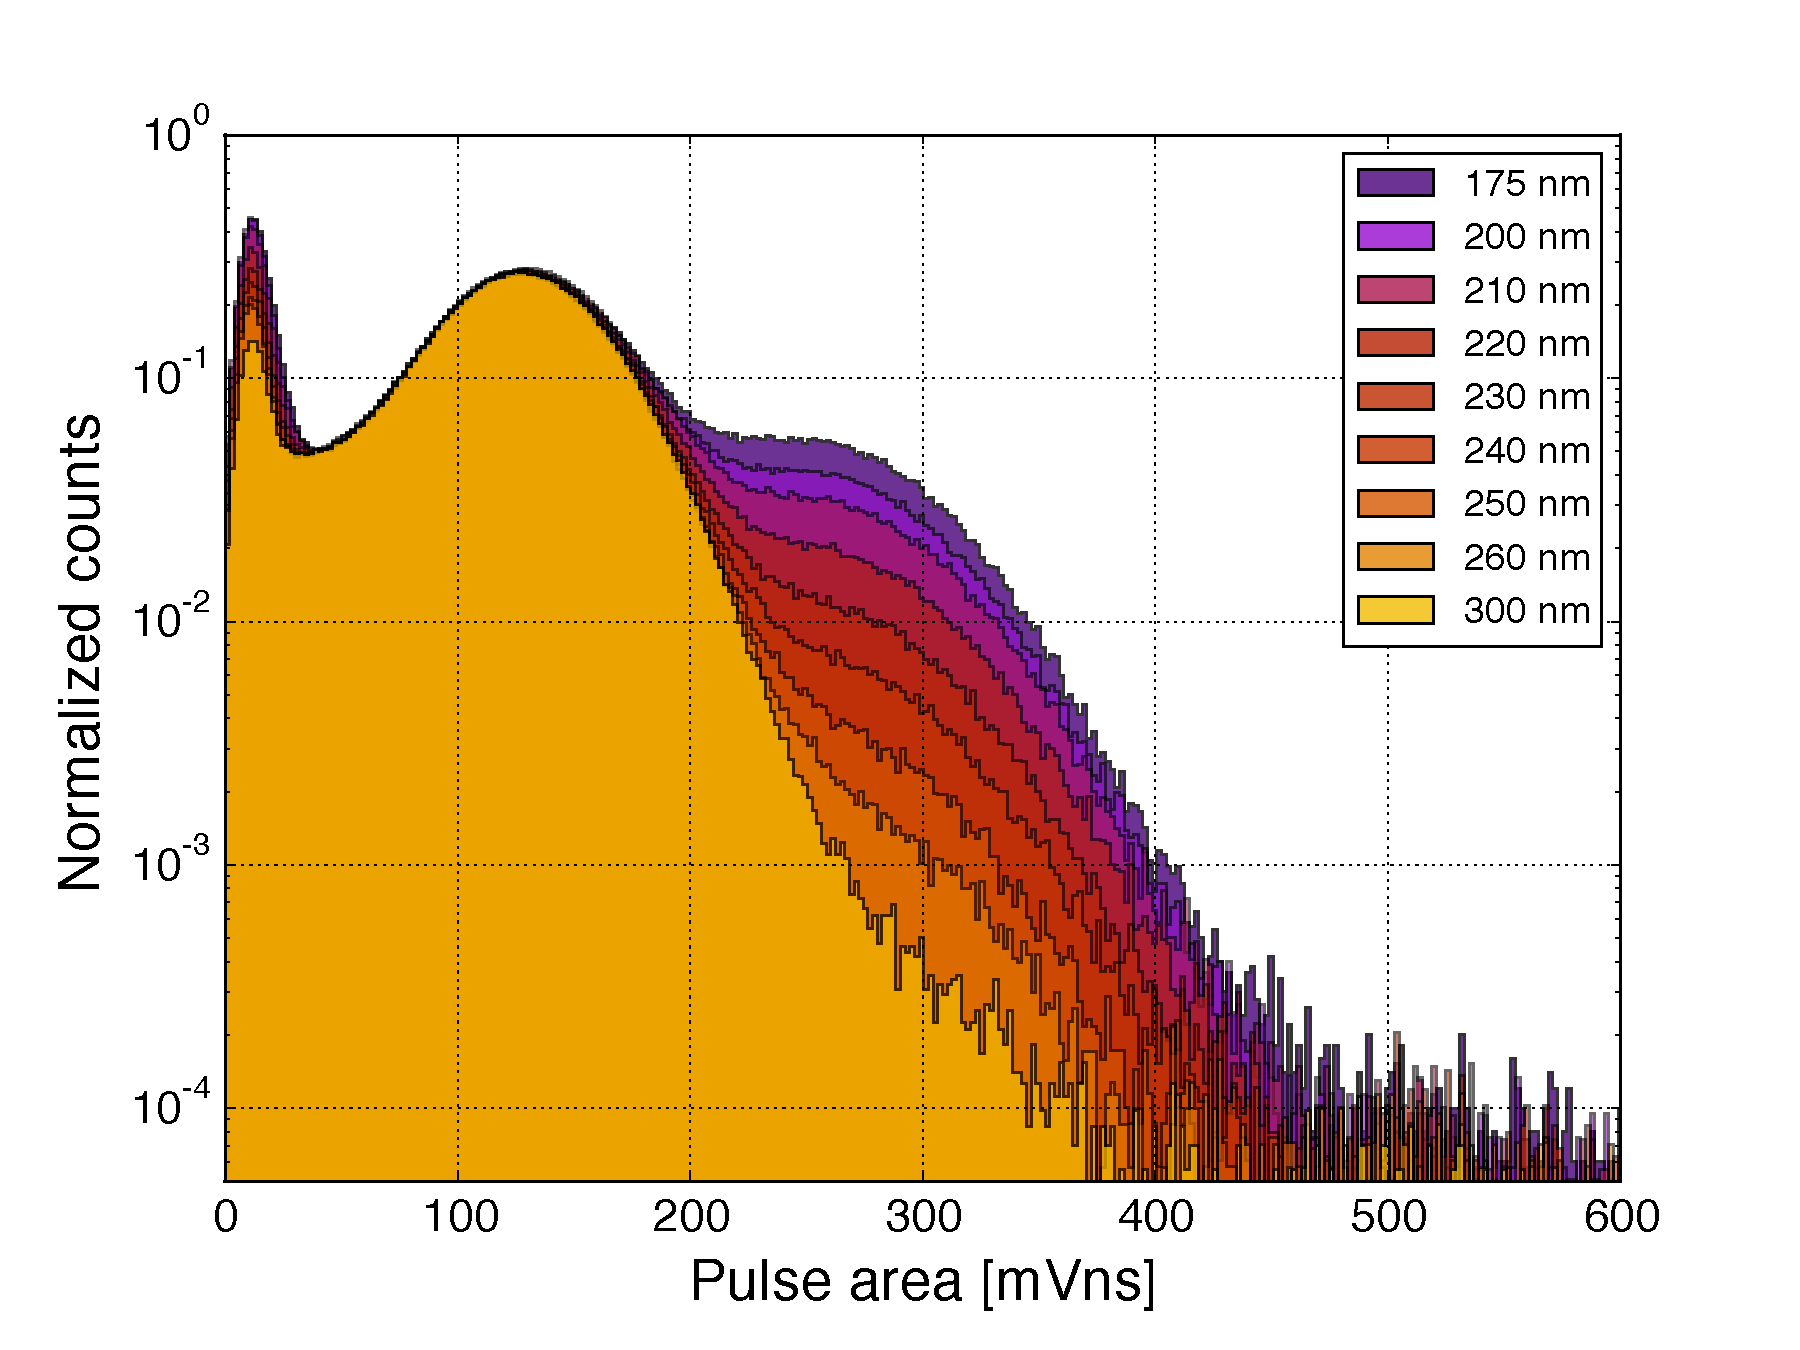
\includegraphics[width=0.99\columnwidth]{fig_R11410_rainbow_plot.pdf}
\caption{Superposition of single photon pulse area spectra of a R11410 PMT for different wavelengths. Each spectrum is normalized by the integral in the region between 50--120~mV~ns in order to show the effect more clearly. Figure from~\cite{Faham:2015kqa}.}
\label{fig:R11410_rainbow_plot}
\end{center} 
\end{figure}

This so-called Double Photoelectron Emission (DPE) effect can therefore be exploited to increase the signal efficiency beyond the standard $n$-fold optimisation, provided that the DPE fraction and efficiency gain can be properly calibrated. This requires the precise determination of the PMT DPE probability, which depends strongly on the wavelength of the impinging light, as well as on the composition and thickness of the photocathode. For the Hamamatsu R11410 PMT model (used e.g.~in XENON1T, XENONnT, RED, and LZ), a wavelength scan was performed with single photons down to the VUV range on one unit~\cite{Faham:2015kqa} (see \autoref{fig:R11410_rainbow_plot}). The inter-PMT variability due to the photocathode manufacturing process has also been measured at low temperature with a batch of 35 R11410-22 PMTs~\cite{Paredes:2018hxp}. Measuring the DPE probability is also crucial for pulse area calibration. A pulse area in `photoelectrons' does not represent the number of photon hits detected, but can be understood and calibrated if the DPE probability is known. Experiments have reported average values of their PMT DPE probability of around $\sim$10--20\% given liquid xenon scintillation light~\cite{Araujo:2020rwg, Akerib:2019zrt}.

\begin{figure}[!htbp]  
\begin{center}
\includegraphics[width=0.99\columnwidth]{fig_LUX_DPE_limits.eps}
\caption{90\%~CL upper limits on the spin-independent WIMP-nucleon cross section obtained using the single-photon population producing Double Photoelectron Emission in the LUX 2013 WIMP search. The observed limit with a 0.3~keV NR energy cut-off is shown in solid black, with 1$\sigma$ and 2$\sigma$ sensitivity bands shown in green and yellow. The dashed black line is derived from the same analysis but with a model cut-off at 1.1~keV. Both of these results correspond to the NEST v.2.0.0 model. The upper limit using a 0.3~keV NR energy cut-off with the newer NEST v.2.0.1 model is shown using a dotted black line. Also shown are other results current at the time, namely from the LUX 2013 search~\cite{Akerib:2015rjg} (gray), the LUX complete exposure~\cite{Akerib:2016vxi} (red), DarkSide-50~\cite{Agnes:2018ves} (green), PandaX-II~\cite{Cui:2017nnn} (blue), PICO60~\cite{Amole:2017dex} (lilac) and CDMSLite~\cite{Agnese:2015nto} (purple). Figure from~\cite{Akerib:2019zrt}.}
\label{fig:lux_DPE_limits}
\end{center} 
\end{figure}

The LUX experiment exploited this DPE to lower the coincidence condition from two PMTs to just a single PMT with an S1 pulse consistent with DPE~\cite{Akerib:2019zrt} (\autoref{fig:lux_DPE_limits}). In general, an experiment may lower its $n$-fold condition by requiring that a subset of PMT hits are consistent with DPE. A PMT with a low dark count rate and high DPE probability might enhance the low-energy reach of a next-generation dark matter experiment with a straightforward extension of the analysis~\cite{Akerib:2021pfd}.

\subsection{Charge-Only Analysis}\label{sec:s2only}

Interactions from WIMP candidates below $\sim\n{GeV/c^2}$ would produce scintillation (S1) signals close to or below the typical low-energy threshold of liquid xenon TPCs. This loss of efficiency can be bypassed by removing the requirement that the S1 signal be detected at all, and leveraging the inherent gain in the S2 signal~\cite{Aprile:2016wwo, Agnes:2018ves, Aprile:2019xxb, Akerib:2021pfd}. Relaxing the requirement of an observed S1 allows events which resulted in even a single extracted electron to be analyzed. This increased sensitivity to low-mass dark matter candidates comes at the expense of particle discrimination (usually from the S2/S1 ratio) and accurate determination of the z-coordinate (usually from the delay between the S1 and S2 signals). While sometimes these analyses still make use of S1 pulses to reject background events, when they do not require an S1 to be present, they are commonly referred to as `charge-only' or `S2-only' analyses.

Thus far, charge-only analyses have been background-limited due to large single- and few-electron backgrounds, which have yet to be reliably quantified and mitigated~\cite{Akerib:2020jud, Kopec:2021ccm, Bodnia:2021flk, Akimov:2016rbs, Aprile:2013blg, Sorensen:2017kpl, Sorensen:2017ymt}. The extended drift volume of a next-generation detector may be subject to stronger electron lifetime effects, but will also provide improved identification of S2s originating from the bottom of the detector because of increased electron diffusion (resulting in wider S2 pulses). Additionally, xenon contamination from out-gassing or surface detachment of impurities will benefit from the relative scaling of volume and surface area. Despite being background limited, charge-only analyses have been used to set leading limits on dark matter interaction rates, see \autoref{fig:sub_GeV}. The sensitivity of liquid xenon TPCs to signals at the level of single electrons results in leading sensitivity to sub-GeV WIMPs as well as other particle models. A charge-only analysis in a next-generation detector will further improve this sensitivity over the current generation of xenon TPCs. 

\begin{figure}[!htbp] 
\begin{center}
\includegraphics[width=0.99\columnwidth]{fig_x1t_subGeV.pdf}
\caption{The 90\% confidence level upper limits (black lines with gray shading above) on spin-independent dark matter-nucleus scattering with the dark matter mass, $m_\chi$, on the horizontal axis. The thick black line is the result from the XENON1T charge-only analysis. Other results from XENON1T in blue~\cite{Aprile:2018dbl}, LUX in orange~\cite{Akerib:2016vxi}, PandaX-II in magenta~\cite{Ren:2018gyx}, DarkSide-50 in green~\cite{Agnes:2018ves}, XENON100 in turquoise~\cite{Aprile:2016wwo, Aprile:2016swn}. Dotted lines show the XENON1T limit when assuming the $Q_y$ from NEST v2.0.1~\cite{szydagis_m_2019_3357973} cut off below 0.3~keV. The limits exhibit a steep change at 17.5~GeV$/c^2$ because the observed count changes from 10 to 3 events in the ROIs left and right of this change, respectively. Figure taken from~\cite{Aprile:2019xxb}.}
\label{fig:sub_GeV}
\end{center} 
\end{figure}

\subsection{General Dark Matter-Induced Atomic Responses}\label{sec:genatomresp}

A dark matter particle with mass in the MeV--GeV range can deposit enough energy in the collision with an electron in a xenon atom to ionise the target and produce a detectable S2 signal in a TPC detector~\cite{Kopp:2009et,Essig:2011nj}. This charge-only analysis has mainly been performed with models where the interaction between dark matter and electrons is mediated by a new hypothetical force carrier such as the dark photon~\cite{Agnes:2018oej,Aprile:2019xxb}. To avoid confusion, here the dark photon acts as force carrier, as opposed to the analysis described in \autoref{sec:dark_photon}, where the dark photon itself is the dark matter candidate. In this framework, the total ionisation rate for a given xenon orbital can be expressed in terms of a single target-dependent ionisation form factor, which is a function of the initial and final state electron wave functions~\cite{Kopp:2009et,Essig:2011nj}.

Xenon detectors can also probe more complex models, such as those where the amplitude for dark matter scattering by a free electron, $\mathcal{M}$, depends on the initial electron momentum~\cite{Catena:2019gfa}. These include models where dark matter couples to electrons via magnetic dipole or anapole interactions. By expanding $\mathcal{M}$ using effective theory methods similar to the ones previously discussed in the context of dark matter-nucleon interactions (see \autoref{sec:nreft}), Reference~\cite{Catena:2019gfa} found that the most general form for the total ionisation rate of a given xenon orbital is a linear combination of four target-dependent atomic responses, which are defined in terms of initial and final state electron wave function overlap integrals. Assuming that dark matter is made of fermions with mass in the MeV-GeV range and interactions dominated by electromagnetic moments of higher order, such as the electric and magnetic dipoles or the anapole moment, reference~\cite{Catena:2020tbv} showed that liquid xenon TPCs can shed light on whether dark matter is a Dirac or Majorana particle. By using Monte Carlo simulations and a non-trivial extension of the likelihood ratio test to the case where one of the hypotheses lies on the boundary of the parameter space, only about $45-610$ signal events are required to reject Majorana dark matter in favour of Dirac dark matter at 3~sigma confidence level. 

\subsection{Migdal Effect and Bremsstrahlung}\label{sec:migdal}

\begin{figure}[!htbp] 
\begin{center}
\includegraphics[width=0.99\columnwidth]{fig_x1t_migdal.pdf}
\caption{Limits on the spin-independent light mediator dark matter-nucleon interaction cross section at 90\% confidence level using signal models from the Migdal effect and Bremsstrahlung in the XENON1T experiment with the S1-S2 data (blue contours and lines) and charge-only data (black contours and lines). The solid and dashed (dotted) lines represent the lower boundaries (also referred to as upper limits) and Midgal (Bremsstrahlung) upper boundaries of the excluded parameter regions. Green and yellow shaded regions give the 1 and 2$\sigma$ sensitivity contours for upper limits derived using the S1-S2 data, respectively. The upper limits on the spin-independent dark matter-nucleon interaction cross sections from LUX~\cite{Akerib:2018hck} and XENON1T charge-only (elastic nuclear recoil results)~\cite{Aprile:2019xxb} are also shown. Figure taken from~\cite{Aprile:2019jmx}.}
\label{fig:migdal}
\end{center} 
\end{figure}

\begin{figure}[!htbp]
    \includegraphics[width=0.99\columnwidth]{fig_migdal_s2o_projection.pdf}
    \caption{Spin-independent sensitivity for the electronic recoil-inducing Migdal effect for the case of a heavy scalar mediator. The S1-S2 sensitivity (black, solid) and the charge-only sensitivity (violet, solid) are shown. The charge-only analysis improves the sensitivity by more than two orders of magnitude with respect to the standard S1-S2 analysis (red, solid). Experimental limits from similar analyses in LUX (blue, solid)~\cite{Akerib:2018hck}, XENON1T (green, solid)~\cite{Aprile:2019xxb} and CDEX (gray, solid)~\cite{Liu:2019kzq} are also shown.\label{fig:migdalProjection}}
\end{figure}

The progressive loss of the scintillation (S1) response with decreasing nuclear recoil energy impede the ability of liquid xenon TPCs to reach sensitivity for sub-GeV dark matter masses. However, the standard dark matter-nucleus interaction can also induce an inelastic atomic scattering signal. 
The Migdal effect~\cite{Migdal:1941} predicts the ionization of the atom with some (small) probability due to the sudden nuclear acceleration caused by the dark matter collision, resulting in excitation and ionization processes from the electrons~\cite{Ibe:2017yqa}. Since electronic recoils produce a more detectable signal than nuclear recoils, this channel enables liquid xenon detectors to reach dark matter masses of $\mathcal{O}(100\ {\textrm{MeV}/c^2})$~\cite{Dolan:2017xbu,Akerib:2018hck,Aprile:2019jmx}, see \autoref{fig:migdal}. The sensitivity of liquid xenon detectors to sub-GeV dark matter achieved using the Migdal effect is competitive with other detectors that are dedicated to searches of light dark matter~\cite{NEWS-G:2017pxg,CRESST:2019jnq,SuperCDMS:2020ymb}. \autoref{fig:migdalProjection} shows a conservative projected Migdal sensitivity for a next-generation detector assuming LZ detector parameters with an extended exposure of 300~tonne-years, equivalent to e.g.~a 56~tonne fiducial mass and 5.4~live-years. 

Similar to the Migdal effect, nuclear Bremsstrahlung searches leverage the fact that in liquid xenon at low energies, electronic recoils produce a stronger signal than nuclear recoils~\cite{Kouvaris:2016afs}. Bremsstrahlung searches consider the emission of a photon from the recoiling atomic nucleus. In the atomic picture this can be viewed as the dipole emission of a photon from a xenon atom that has been polarized in the dark matter-nucleus scattering. In xenon, the emission of the Bremsstrahlung photon is more heavily suppressed compared to the Migdal effect and hence results in a weaker signal. The theoretical motivation and event rates for Bremsstrahlung have been derived in~\cite{Kouvaris:2016afs} and searches using liquid xenon detectors have been published in~\cite{Akerib:2018hck,Kobayashi:2018jky,McCabe:2017rln}.

\subsection{Hydrogen Doping}\label{sec:hydrodoping}

Kinematically, the large xenon nucleus (average mass 122~GeV) is not well suited for an efficient transfer of energy from Galactic dark matter with mass $\lesssim$1~GeV/$c^2$. As a result, nearly all of the resulting xenon nuclear recoils fall below the energy threshold for detection. A possible solution for enhancing the sub-GeV sensitivity of liquid xenon TPCs is to dissolve a lighter species in the liquid xenon bulk~\cite{Akerib:2021hydrox}. In this configuration, the lighter nucleus becomes the dark matter target, and the xenon becomes the sensing medium.

This strategy exploits two of the primary advantages of the liquid xenon medium. First, the high atomic number and density of liquid xenon provides excellent self-shielding of external backgrounds from the central volume of the detector. Such a suppression would not be possible in a similarly-sized detector comprised of the light species alone. Second, the high yield of detectable quanta (electrons and photons) resulting from low-energy particle interactions makes xenon an ideal sensor for the recoiling light nuclei.

Having the lightest nucleus of any element, hydrogen is kinematically the best candidate species for detecting sub-GeV dark matter interactions. The lone proton comprising hydrogen's nucleus additionally provides unique sensitivity to the spin-dependent dark matter coupling to protons. Likewise, doping the xenon target with deuterium would provide similar sensitivity to the neutron-only couplings. Helium is also a viable option as the light mass target species, but its spin-dependent sensitivity would be comparatively poor. Introduction of helium into the detector might not be suitable if PMTs are used as a photosensor due to its ability to diffuse into and degrade the PMT vacuum. However, helium could be considered as a dopant if silicon photomultipliers (SiPMs) are used to detect light signals instead of PMTs.

\subsection{Upscattered Dark Matter}\label{sec:upscattdm}

The sensitivity reach of liquid xenon detectors for sub-GeV dark matter is significantly enhanced if some dark matter particles receive a kinematic boost from up-scattering with cosmic rays~\cite{Bringmann:2018cvk,Alvey:2019zaa,Cappiello:2019qsw,Dent:2019krz,Bondarenko:2019vrb,Wang:2019jtk}. This process, often denoted CRDM, will create a small population of fast or even relativistic dark matter particles. This in turn provides sensitivity to liquid xenon experiments to dark matter with masses several orders of magnitude below 1~GeV. Cosmic ray up-scattered dark matter is only a fraction of the Galactic dark matter population, with an abundance and flux that depends on the dark matter-cosmic ray scattering cross section, the local dark matter density, and the local interstellar spectrum of cosmic rays. Relatively large cross section values of e.g. $\sigma_{\chi N}\gtrsim 10^{-31}{\rm{cm}}^2$ for $m_\chi = 1$~GeV are required to have a notable impact on the sensitivity of a typical liquid xenon detector. For spin-independent interactions, liquid xenon experiments are competitive with and complementary to existing neutrino experiments~\cite{Bringmann:2018cvk, Cappiello:2019qsw,  PROSPECT:2021awi}, which have sensitivity in a similar region of parameter space.

Another upscattering mechanism extending the sensitivity of liquid xenon detectors to dark matter masses down to keV scales is a process called ``solar reflection''~\cite{An:2017ojc,Emken:2017hnp}. This is based on the observation that scatterings on thermal electrons and nuclei within the Sun can accelerate light dark matter particles. This could give rise to an observable flux of highly energetic particles in a liquid xenon TPC detector.

\subsection{Dark Matter Annihilation Products}\label{sec:dmproducts}

In several models of so-called ``neutrino portal" dark matter, Galactic dark matter self-annihilates into neutrinos~\cite{Cherry:2014xra,GonzalezMacias:2015xbi,Becker:2018rve,Lamprea:2019qet,Patel:2019zky}. These in turn may be detected at direct detection experiments with high rates via coherent elastic neutrino-nucleus scattering (see \autoref{sec:cevns}). A next-generation liquid xenon detector would be sensitive to the flux of these neutrinos for dark matter mass (respective neutrino energy) of $[0.01-1]\1{GeV/c^2}$~\cite{McKeen:2018pbb}. The sensitivity to this neutrino flux would complement neutrino detectors such as Super-Kamiokande. Similarly, dark matter that annihilates to a second component of nucleophilic, ``boosted" dark matter could also be discovered. A next-generation liquid xenon TPC will be sensitive to the effective baryonic coupling of thermal boosted dark matter that is as low as the weak interaction~\cite{McKeen:2018pbb}.

Alternatively, dark matter may annihilate or decay within the target volume of future liquid xenon detectors~\cite{Undagoitia:2021tza}. Considering deposited energies up to a few MeV, the relevant final states include annihilation into $\gamma\gamma$ and $e^-e^+$, and decays into $\gamma\gamma$, $\gamma\nu$ and $e^-e^+$. Although the sensitivity obtained is not as high as the current limits from cosmological considerations~\cite{Slatyer:2015jla} and X-ray measurements~\cite{Ng:2019gch}, this is a complementary approach in a well-understood background environment and free of the large uncertainties typically present in indirect detection experiments.

\subsection{Bosonic Super-WIMPs}\label{sec:bosonicwimp}

Super Weakly Interacting Massive Particles, or super-WIMPs, make up a broad class of dark matter candidates that couple to Standard Model particles with cross sections far smaller than the weak scale~\cite{Feng:2003xh}. These include fermions such as sterile neutrinos~\cite{Dodelson:1993je} and gravitinos, both of which only couple to the Standard Model gravitationally and thus are impossible to observe in a typical direct detection experiment. However, keV-scale bosonic super-WIMPs can couple to light Standard Model particles in such way to be observed with low-background experiments~\cite{Pospelov:2008jk}. Here we give two examples of super-WIMPs, dark photons and axion-like particles, and discuss related signals.

\subsubsection{Dark Photons}\label{sec:dark_photon}

Dark photons are vector bosonic super-WIMPs. Proposed as a force carrier for a dark sector, they can also serve as a dark matter candidate if they are stable enough~\cite{Pospelov:2008jk}. The dark photon kinetically mixes with the SM photon, and can be absorbed in a detector medium with a cross section proportional to the photoelectric cross section. The expected signal is therefore a mono-energetic electronic recoil peak at the dark photon mass. Direct detection experiments have set competitive constraints on kinetic mixing parameter $\kappa$ of dark photons, in a mass range from several to hundreds of keV~\cite{An:2014twa}. A next-generation detector such as the one discussed here will have improved sensitivity to this mixing parameter $\kappa$. Further, dedicated low-energy calibrations, for example using $^{37}$Ar diluted in the liquid xenon, will help to improve the search in the keV mass range and reduce the relevant detector-specific systematics to negligible levels for a discovery experiment. Using a low-energy charge-only analysis (\autoref{sec:s2only}), the sensitive mass range can be extended to the sub-keV level.

\subsubsection{Axions and Axion-Like Particles}

The axion is a pseudoscalar Goldstone boson originally proposed as a solution to the strong CP problem of QCD~\cite{PecceiQuinn_1977,Weinberg:1977ma,Wilczek:1977pj}. Stable and massive, axions are also well-motivated dark matter candidates~\cite{Preskill:1982cy,Abbott:1982af,Dine:1982ah}. They couple to the Standard Model very weakly, with couplings suppressed by a high energy scale $f_a$. QCD axions -- i.e. axions that also solve the strong CP problem -- have couplings $g \sim 1/f_a$ that are proportional to the axion mass $m_a$ which is constrained to be $m_a \lesssim 1\1{eV/c^2}$ by astrophysical bounds~\cite{Raffelt:2006cw,Sikivie:2006ni,Ayala:2014pea,Chang:2018rso,Capozzi:2020cbu} and the solar axion helioscope CAST~\cite{Anastassopoulos:2017ftl}. Such axions are below the sensitivity reach of detectors like the one discussed here, and require dedicated experiments. However, axions produced in the Sun would have thermal spectra with keV energies, and could be detected with a xenon TPC as discussed in \autoref{sec:solar_axions}.

Axion-like particles (ALPs) are the phenomenological generalization of the QCD axion in that they share the same properties, but the strict relationship between the mass and the scale $f_a$ is relaxed. These particles do not solve the strong CP problem, but nevertheless are good dark matter candidates and can show up abundantly in theories for physics beyond the standard model, in particular string theory~\cite{Witten:1983ar,Conlon:2006tq,Arvanitaki:2009fg,Arvanitaki:2010sy,Cicoli:2012sz, Arvanitaki:2014wva}. In a similar way to dark photons, ALPs can be detected via an analogous process to the photoelectric effect~\cite{Derevianko:2010kz}. For dark matter ALPs, the resulting signal is again a mono-energetic spectrum of electronic recoils at the ALP mass, with an event rate proportional to the square of the dimensionless axion-electron coupling~$g_{ae}$. 

Due to their ultra-low electronic recoil background levels, liquid xenon TPCs have placed the strongest constraints to date on keV ALP dark matter~\cite{Aprile:2014eoa, Abe:2014zcd,Akerib:2017uem, Fu:2017lfc,Abe:2018owy,Aprile:2019xxb,Aprile:2020tmw,Zhou:2020bvf}, and next generation detectors will likely continue to set world-leading constraints~\cite{Aalbers:2016jon}.

\subsubsection{Solar Axions, Dark Matter, and Baryon Asymmetry}

As discussed in \autoref{sec:solar_axions}, a liquid xenon TPC can detect the QCD axion and axion-like particles from the Sun for sufficiently large couplings of the axion with electrons or photons. Such relatively large couplings correspond to a small decay constant of the axion. In this case, the cosmological abundance of axions produced by conventional mechanisms~\cite{Abbott:1982af,Dine:1982ah,Preskill:1982cy,Davis:1986xc} is too small for the axion to explain the observed dark matter. However, the axion abundance can be large enough to be dark matter in the various scenarios proposed in~\cite{Sikivie:1982qv,Visinelli:2009kt,Hiramatsu:2010yn,Co:2017mop,Co:2018mho,Co:2019jts,Hook:2019hdk}, with couplings that are sufficiently large to be detected in the proposed detector. 

In one such cosmological scenario for example~\cite{Co:2019jts}, a non-zero field velocity delays the onset of field oscillations, enhancing the axion abundance relative to the conventional misalignment mechanism. For axion-like particles, this field velocity can simultaneously explain the baryon asymmetry of the universe~\cite{Co:2020xlh}. Fitting the ratio of dark matter to baryon abundances predicts the axion coupling in terms of its mass $m_a$
\begin{equation}
g_{a \gamma} \simeq 2\times 10^{-11}c_\gamma~{\rm GeV}^{-1} \left(\frac{m_a}{\rm meV}\right)^{1/2},
\end{equation}
where $c_\gamma$ is a model-dependent constant of order unity. For any axion mass, this is much larger than the photon coupling of the QCD axion. A next-generation liquid xenon TPC with a 1000 ton-year exposure can probe this coupling down to $g_{a\gamma}\sim 3 \times 10^{-11} {\rm GeV}^{-1}$~\cite{Dent:2020jhf}, corresponding to $m_a \sim$~meV.

\subsection{Luminous Dark Matter}\label{sec:lumidm}

It is possible to construct models where the dominant signal of the dark matter originates from photons. These photons could be observed in direct detection experiments as a monoenergetic line produced by dark matter decay from an excited state~\cite{Feldstein:2010su,Pospelov:2013nea}. The excited state could be populated through upscattering in or near the detector (and have short lifetimes $\sim1\,\mu s$) or in the Earth (lifetimes $\sim(1-10)$\,s). For this scenario to work, the elastic cross section needs to be small relative to the inelastic cross section. A simple way to achieve this is with a magnetic dipole operator which couples two distinct Majorana fermions that have a small, $\mathcal{O}$(keV) mass splitting. Such "Luminous dark matter" was first proposed as a potential explanation of the DAMA/LIBRA modulation~\cite{Feldstein:2010su} and has since been used to explain the recent XENON1T excess~\cite{Bell:2020bes}. While the former scenario is now strongly constrained, the latter scenario will be confirmed or ruled out by a next-generation liquid xenon experiment.

\subsection{Mirror Dark Matter}\label{sec:mirrordm} % both ER and NR

Mirror Dark Matter~\cite{Foot:2007nn} represents the intriguing idea that an exact copy of the Standard Model in the dark sector is invoked with an unbroken symmetry between the two. Mirror dark matter can generate signatures both in nuclear recoils similar to those expected from $\sim 7\1{GeV}/c^2$ WIMPs with a cross section around $10^{-44}\1{cm^2}$, as well as in electronic recoils~\cite{Foot:2010hu,Foot:2014mia,Foot:2018jpo}. Mirror dark matter as a hypothesis is potentially entirely falsifiable by a next-generation liquid xenon experiment~\cite{Clarke:2016eac}.

\subsection{Magnetic Inelastic Dark Matter}\label{sec:maginelasticdm}

A natural scenario where dark matter dominantly scatters off nuclei through an inelastic transition in the dark sector (\autoref{sec:inelasticdarkmatter}) is the case of a magnetic dipole interaction~\cite{Chang:2010en}. This model relies on the fact that fermionic dipole operators vanish for Majorana fermions. Thus, if a dark matter Dirac fermion state is split into two nearly degenerate Majorana fermions, an elastic dipole transition is forbidden, leaving the leading dark matter interaction to be an inelastic magnetic dipole transition. Many examples of dark matter models that can realize this scenario have been studied, see e.g.~\cite{Kumar:2011iy,Patra:2011aa,Weiner:2012gm, Pierce:2014spa}.   

For magnetic inelastic dark matter, the sensitivity of a direct detection experiment is modified by both the kinematic constraints of inelastic transitions and by the dependence on the charge and magnetic dipole moment of the target nuclei~\cite{Chang:2010en}. Depending on the dark matter mass splitting and the size of the dipole moment, the excited dark matter state can also decay in the detector, thus yielding both a nuclear recoil from the initial scatter and an electronic recoil from the decay shortly thereafter. Searching for the photons produced by this decay can be an additional handle on uncovering such a scenario~\cite{Lin:2010sb, Pospelov:2013nea}. A dedicated search has been performed by XENON100~\cite{Aprile:2017kek}, with the proposed experiment providing significantly improved sensitivity not only due to the lower background and longer exposure, but also due to the larger size of the detector which translates into a sensitivity to longer decay times.

\subsection{Dark Matter around the Planck Mass} \label{sec:planck}

\begin{figure}[!htbp]  
\begin{center}
\includegraphics[width=0.99\columnwidth]{fig_multiscatter_SI.pdf}
\caption{Per-nucleon spin-independent scattering cross sections and dark matter masses that can be probed by liquid xenon dark matter detectors via dedicated searches for multi-scatter signals. For cross sections above $\sigma_{\rm MIMP}$ (horizontal green lines) one expects dark matter to scatter multiple times in the detector while transiting. The maximum mass reachable (vertical green lines) is limited by the total integrated flux of dark matter in the detector over the run-time of the experiment. Masses up to and beyond the Planck mass $\simeq 10^{19}\1{GeV/c^2}$ may be probed with a next-generation detector. Figure taken from~\cite{Bramante:2018qbc}.}
\label{fig:multiscatter_SI}
\end{center} 
\end{figure}

The observed local dark matter mass density could be made up of few but very massive dark matter particles with masses around the Planck mass $\simeq 10^{19}\1{GeV/c^2}$, as opposed to numerous lighter particles. Super-massive species are motivated by supersymmetric and grand unified theories~\cite{Kolb:2017jvz}, and their detection could help determine parameters of the early universe such as inflation~\cite{Chung:1998zb}. Their existence could also imply new light mediators beyond the Standard Model~\cite{Davoudiasl:2018wxz}. 

Due to the small number density, the flux of these particles through a given detector would be very low, and thus any detection would both imply and require a very high scattering cross section, such that almost all particles impinging on the detector prompt a signal. When the cross section becomes high enough that these particles would interact more than once in the detector, discovery requires a dedicated analysis looking for multiple-scatter events. Such events are typically discarded in WIMP-like dark matter analyses, leaving many orders of magnitude of unexplored parameter space, see \autoref{fig:multiscatter_SI}. In this multiple scattering regime, a next-generation liquid xenon experiment would be capable of probing dark matter masses up to and beyond the Planck mass $\simeq 10^{19}$~GeV~\cite{Bramante:2018qbc}, in a complementary way to the range that could be probed using dedicated neutrino experiments~\cite{Bramante:2018tos,Clark:2020mna}.
Clusters of dark matter formed through self-attraction~\cite{Butcher:2016hic}, such as ``dark blobs''~\cite{Grabowska:2018lnd} or ``dark nuggets''\cite{Coskuner:2018are} would also be visible as tracks in the detectors.



\section{Double Beta Processes}\label{sec:doublebeta}

\subsection{Neutrinoless Double Beta Decay of \texorpdfstring{$^{136}$Xe}{Xenon-136}} \label{sec:0nubb}

Among the main intellectual challenges facing the nuclear and particle physics communities today are the neutrino-mass generation mechanism, the absolute neutrino-mass scale, and the neutrino-mass spectrum. One of the best ways to address these fundamental questions is to search for neutrinoless double beta decay ($0\nu\beta\beta$)~\cite{Avignone:2007fu, Dolinski:2019nrj}. The observation of this rare nuclear decay process, forbidden in the Standard Model, would imply that the lepton number is violated by two units and confirm the Majorana nature of the neutrinos. Double beta decay can occur in the two xenon isotopes $^{134}$Xe~\cite{LZ:2021rff} and $^{136}$Xe, with the latter offering a larger sensitivity to the $0\nu\beta\beta$ half-life ($T^{0\nu}_{1/2}$). The best experimental constraint on the $^{136}$Xe $0\nu\beta\beta$ half-life, $T^{0\nu}_{1/2} > 1.07 \times 10^{26}\1{years}$ (90\% CL), is set by the KamLAND-Zen collaboration using $^{136}$Xe dissolved in a liquid scintillator~\cite{KamLAND-Zen:2016pfg}. The EXO-200 collaboration demonstrated that better energy resolution and background rejection can be achieved with a liquid xenon TPC~\cite{Albert:2017owj}, and the PandaX-II collaboration conducted a first search using a dual-phase natural xenon detector~\cite{Ni:2019kms}. XENON1T recently demonstrated that energy resolutions below $\sigma/\mu=1$\% at $Q_{\beta\beta}$ can be achieved in liquid xenon TPCs used for dark matter searches~\cite{XENON:2020iwh}.

\begin{figure}[!htbp]
\begin{center}
\includegraphics[width=0.99\columnwidth]{fig_0vbb_signal.png}
\caption{Predicted  background  spectrum around the $0\nu\beta\beta$ energy region of interest (ROI) for a proposed next-generation dark matter experiment. Rates are averaged over a fiducial volume (FV) containing $5000\1{kg}$ of liquid xenon with natural isotopic abundance. Bands indicate $\pm~1\sigma$ uncertainties. Figure from~\cite{Agostini:2020adk}.}\label{fig:0vbb_signal}
\end{center}
\end{figure}

A next-generation liquid xenon detector will contain multiple tonnes of the $^{136}$Xe isotope, either at the natural abundance of 8.9\%, or, as a possible upgrade, using enriched xenon. Given a TPC design optimized for WIMP searches, a detector instrumenting $\sim 40,000\1{kg}$ of non-enriched xenon can already improve the sensitivity to $0\nu\beta\beta$ decay by more than one order of magnitude over current limits, without any interference with its primary dark matter science goal. Taking advantage of the excellent self-shielding of liquid xenon, the material-induced gamma ray background can be suppressed below the total intrinsic background rate (\autoref{sec:erfiducialization}. \autoref{fig:0vbb_signal} shows the relevant sources of background with a hypothetical $0\nu\beta\beta$ signal for the innermost $5000\1{kg}$ of natural xenon in the TPC of a proposed next-generation detector~\cite{Agostini:2020adk}. The background from material-induced gamma rays will be further reduced in more massive detectors than the one simulated in \autoref{fig:0vbb_signal}.

\begin{figure}[!htbp]
\begin{center}
\includegraphics[width=0.99\columnwidth]{fig_0vbb_acceptance.png}
\caption{Efficiency of $0\nu\beta\beta$ signal acceptance and background rejection as a function of the minimum distance for individual reconstruction of energy depositions. The three signal lines (blue) compare different energy and angular distributions for the $0\nu\beta\beta$ signal based on a back-to-back electron emission, a mass mixing (MM) mechanism and a right-handed current (RHC) model. The background rejection efficiency is shown for $\gamma$s (red) and electrons (green) with $E=Q_{\beta\beta}=2457.8\1{keV}$. The vertical line (gray) corresponds to the value assumed here. Bands indicate $\pm~2\sigma$ uncertainties~\cite{Agostini:2020adk}.}\label{fig:0vbb_acceptance}
\end{center}
\end{figure}

\begin{figure}[!htbp]
\begin{center}
\includegraphics[width=0.99\columnwidth]{fig_0vbb_sensitivity.png}
\caption{Predicted median $T_{1/2}^{0\nu}$ sensitivity at 90\%~CL as a function of the exposure time for a next generation TPC detector containing \SI{40}{t} of liquid xenon with natural isotopic abundance. The band indicates the sensitivity range between a baseline radio purity scenario at a depth of \SI{3500}{m} water equivalent to a scenario with neutrino dominated background. Sensitivity projections for future $^{136}$Xe $0\nu\beta\beta$ experiments~\cite{Agostini:2020adk, Gomez_NEXT:2019, Chen:2016qcd, Albert:2017hjq, Barabash:2015eza} are shown for comparison.}\label{fig:0vbb_sensitivity}
\end{center}
\end{figure}

Selecting ultra-low background materials for construction can further reduce the material contribution as well as the background rate from $^{222}$Rn, which emanates from material surfaces into the target volume. A sufficiently deep laboratory suppresses cosmogenic background sources, such as the in-situ activation of $^{136}$Xe by muon-induced neutrons (producing $^{137}$Xe)~\cite{Cebrian:2020bwn,Rogers:2020npx}, down to the limit set by electron scattering of solar $^{8}$B neutrinos. Optimizing the detector design for an improved spatial resolution would allow to further exploit background rejection, based on the different topology of background and signal events caused by Bremsstrahlung radiation, as shown in \autoref{fig:0vbb_acceptance}. Combining these measures, the experimental sensitivity can be further enhanced to make a next-generation dark matter detector competitive to dedicated next-generation, tonne-scale $0\nu\beta\beta$ experiments, as shown in \autoref{fig:0vbb_sensitivity}. Isotopic enrichment in $^{136}$Xe would further improve this sensitivity, as it linearly increases the signal, although this also increases the background rate from the two-neutrino double beta decay ($2\nu\beta\beta$) of $^{136}$Xe and $\beta$-decay of $^{137}$Xe.

Besides the search for $0\nu\beta\beta$ decay, precision measurements of the $2\nu\beta\beta$ decay can reduce the experimental uncertainty on the $2\nu\beta\beta$ nuclear matrix and constrain the underlying nuclear theories~\cite{Saakyan:2013yna}.  Recent research shows that precise $2\nu\beta\beta$ spectrum shape measurement can provide insights towards reliable $0\nu\beta\beta$ nuclear matrix element calculations~\cite{KamLAND-Zen:2019imh}. In addition, precision measurements of $2\nu\beta\beta$ decay can also be used to probe New Physics. For example, right-handed lepton currents affect the angular and energy distributions of the decay \cite{Deppisch:2020mxv}, MeV-scale sterile neutrinos can be searched for through kinks in the $2\nu\beta\beta$ spectrum \cite{Bolton:2020ncv, Agostini:2020cpz}, and neutrino self-interactions can leave an imprint on the spectrum as well \cite{Deppisch:2020sqh}. Because lepton number is not necessarily violated in $2\nu\beta\beta$ decay, this is independent of the neutrino nature and can be used to constrain or pinpoint properties of both Majorana and Dirac neutrinos.

\subsection{Double Electron Capture on \texorpdfstring{$^{124}$Xe}{Xenon-124}}\label{sec:dec}

Similar to double beta decay, double electron capture is a second order Weak Interaction process~\cite{Winter:1955zz} with extremely long half-lives. Two electrons are captured from the atomic shell and two protons are converted into neutrons. In the Standard Model decay, two neutrinos carrying virtually the total Q-value are emitted and leave the active volume undetected ($2\nu$ECEC). The measurable signal is constituted by the atomic de-excitation cascade of X-rays and Auger electrons that occurs when the vacancies of the captured electrons are refilled. In a liquid xenon detector, this cascade is measured as a single resolvable signal at $64.3\1{keV}$ for the double K-capture~\cite{Nesterenko:2012xp} as the most likely case~\cite{Doi:1991xf}. The half-life of this decay is of great interest with regard to nuclear matrix element calculations, as it provides a benchmark point from the proton-rich side of the nuclide chart~\cite{Suhonen:2013rca,Pirinen:2015sma,Perez:2018cly}. A precise measurement would help to narrow down uncertainties, which in turn have implications on the neutrino mass scale derived from $0\nu\beta\beta$. 

Following hints in XMASS~\cite{Abe:2018gyq}, the half-life of the $^{124}$Xe double K-capture has recently been measured by XENON1T~\cite{XENON:2019dti}. At $T_{1/2}^{2\nu\text{KK}} = (1.8 \pm 0.5_\text{stat} \pm 0.1_\text{sys}) \times 10^{22}\1{years}$, it agrees with recent theoretical predictions. Assuming a natural isotopic abundance similar to XENON1T, a next-generation experiment would record on the order of 10,000 events in its full exposure. This will allow a precision measurement of the double K-capture half-life to the percent level. Additionally, an observation of the KL-capture and LL-capture would be within reach~\cite{Doi:1991xf}. Their measurement would help to decouple the nuclear matrix element from phase-space factors.

Beyond the Standard Model, the double electron capture on $^{124}$Xe without neutrino emission ($0\nu$ECEC) can complement $0\nu\beta\beta$ in addressing fundamental questions about the mass and nature of the neutrino~\cite{Bernabeu:1983yb,Sujkowski:2003mb}. $^{124}$Xe could allow a resonant enhancement of this channel, which would be needed to provide accessible half-lives~\cite{Kotila:2014zya}. In this case, the decay populates an excited state of the $^{124}$Te daughter nucleus. A suitable daughter state exists, but current measurements of the Q-value indicate only an approximate match of the $^{124}$Te level, two-hole energy, and Q-value that would only provide a minor enhancement~\cite{Nesterenko:2012xp}. If this decay is realized, the experimental signature contains multiple $\gamma$-rays emitted in a cascade, so coincidence techniques could increase experimental sensitivity \cite{Wittweg:2020fak}.

\subsection{Other Double-Beta Processes}

The $^{124}$Xe $Q$-value of 2857~keV also allows second-order decays involving positrons. Examples are the as-yet unobserved Standard Model $2\nu$EC$\beta^+$ and $2\nu\beta^+\beta^+$ decays, as well as the hypothetical $0\nu$EC$\beta^+$ and $0\nu\beta^+\beta^+$ decays. The decay $2\nu$EC$\beta^+$ is predicted to have a half-live one order of magnitude above that of $2\nu$ECEC. Exploiting the coincidence signature of the positron annihilation and the atomic de-excitation cascade, this decay could already be within reach of LZ and XENONnT~\cite{Barros:2014exa, Wittweg:2020fak} and be a sure signal in the next-generation detector. The $2\nu\beta^+\beta^+$ decay exhibits a unique signature with five point-like ionization clusters, located in the same plane with the central vertex~\cite{Bolozdynya:1997pdbd}.

On the neutrinoless side, $0\nu$EC$\beta^+$ would be favoured in the absence of resonance enhancement for $0\nu$ECEC. Here, the current lower limits on the half-lives are on the order of~\SIrange{e25}{e27}{years}~\cite{Barea:2013wga, Kim:1982vi, Doi:1992dm, Hirsch:1994es, Suhonen:2003gx, Rath:2009dr, Wittweg:2020fak}. These would be accessible to a large extent in a next-generation liquid xenon experiment when exploiting the coincidence signature of the atomic relaxation, the mono-energetic positron, and the two subsequent back-to-back $\gamma$-rays. Moreover, limits on half-lives of neutrinoless second-order weak decays in $^{124}$Xe could complement $0\nu\beta\beta$ searches in $^{136}$Xe and help to identify the decay mechanism~\cite{Hirsch:1994es, Wittweg:2020fak}. These channels provide an exciting avenue for the next-generation detector discussed here to complement ongoing searches for double-weak processes.





\section{Neutrinos for Astrophysics} \label{sec:neutrinos}

Many sources of astrophysical neutrinos exist~\cite{Vitagliano:2019yzm,Gann:2021ndb}, and those in the relevant energy range for xenon experiments are shown in \autoref{fig:nufluxes}. Overall, the flux is dominated by pp solar neutrinos, which will be the leading source of low-energy electronic recoils. Atmospheric neutrinos have the highest energy and can induce sizable nuclear recoils of tens of keV through coherent elastic neutrino-nucleus scattering; their measurement is a goal of the next-generation liquid xenon experiment. A prominent source is $^8$B solar neutrinos as they lie in a sweet spot: their energy is high enough that nuclear recoils are visible in dedicated xenon TPCs, while their flux is so large that a first measurement can be achieved already with LZ and XENONnT.

\begin{figure}[!htbp]
\begin{center}
\includegraphics[width=0.99\columnwidth]{fig_nufluxes.pdf}
\caption{Astrophysical neutrino fluxes span many orders of magnitude in flux and energy. This explains the different exposures and energy thresholds required to measure them.}\label{fig:nufluxes}
\end{center}
\end{figure}

A next-generation detector will make important advances in neutrino astrophysics, covering low-energy realms that are out of the reach of experiments such as Hyper-K~\cite{Abe:2018uyc} or DUNE~\cite{Acciarri:2016crz}. This section outlines the scientific scope of the next-generation detector, including solar, atmospheric, and supernova neutrinos, and discusses the unique interaction channels that this detector will be sensitive to. 

\subsection{Neutrino Interactions}

Neutrinos can interact with liquid xenon through Charged Current (CC) and/or Neutral Current (NC) interactions to produce detectable electronic and nuclear recoils. The neutrino-induced rate is
\begin{equation}
\frac{{\rm d}R}{{\rm d}T_R} = \mathcal{N} \times \int_{E_{\nu}^{min}}{\phi\left(E_{\nu}\right) \times \frac{{\rm d}\sigma(E_\nu, T_R)}{{\rm d}T_R} {\rm d}E_\nu}
\end{equation}
where $\mathcal{N}$ is the number of target nuclei or electrons per unit of mass of detector material (for nuclear and electronic recoils, respectively), $\phi\left(E_{\nu}\right)$ is the neutrino flux as a function of the neutrino energy as shown in \autoref{fig:nufluxes}, and $E_{\nu}^{min}$ is the minimum neutrino energy required to generate a recoil at an energy $T_R$. For a nuclear recoil, in the limit where $m_N \gg E_\nu$, the minimum energy is given by 
\begin{equation}
E_{\nu}^{min} = \sqrt{\frac{m_N T_R}{2}},
\end{equation}
whereas in the case of an electronic recoil, it is given by 
\begin{equation}
E_{\nu}^{min} = \frac{1}{2}\left( T_R + \sqrt{T_R\left( T_R + 2m_e \right)}\; \right)
\end{equation}

The differential cross section depends on the nature of the interaction. In the next two sections, we discuss Coherent Elastic Neutrino-Nucleus Scattering and the Electroweak interaction, which constitute the major contributions to the potential detectable signal for liquid xenon detectors.

\subsubsection{Coherent Elastic Neutrino-Nucleus Scattering} \label{sec:cevns}

In the Standard Model, elastic neutrino-nucleon scattering proceeds only through neutral current interaction with the exchange of a $Z$-boson. The resulting differential neutrino-nucleus cross section as a function of the nuclear recoil energy $T_R$ and the incoming neutrino energy $E_\nu$ is
\begin{equation}
\begin{split}
\frac{{\rm d}\sigma(E_\nu, T_R)}{{\rm d}T_R} = \frac{G^2_f}{\pi} m_N  \left( Z g_v^p + N g_v^n \right)^2 \\
\times \left(1 - \frac{m_NT_R}{2E^2_{\nu}}
\right) F^2(T_R)
\end{split}
\end{equation}
where $m_N$ is the target nucleus mass, $G_f$ is the Fermi coupling constant, $N$ the number of neutrons, $Z$ the number of protons, $g_v^n = -1/2$, and $g_v^p = 1/2 - 2 \sin^2 \theta_w$, where $\theta_w$ the Weak mixing angle. Because $\sin^2{\theta_w}\simeq 0.23$, the cross section scales roughly with the number of neutrons squared. The nuclear form factor $F(T_R)$ describes the loss of coherence due to the internal structure of the nucleus. For momentum transfers less than the inverse of the size of the nucleus, the coherence condition is largely satisfied and $F(T_R) \rightarrow 1$. In lieu of experimental data on the neutron distribution in the nucleus, a typical parameterization is the Helm form factor~\cite{Helm:1956zz} that is also commonly used for WIMP direct detection~\cite{Engel:1991wq, Lewin:1995rx}.

\begin{figure}[!htbp]
\begin{center}
   \includegraphics[width=0.99\columnwidth]{fig_nurates.pdf}
   \caption{Nuclear recoil event rates from astrophysical neutrinos via CEvNS. $^8$B solar neutrinos are expected to be measured first in the upcoming LZ and XENONnT experiments. The detector proposed here targets a precision measurement of that flux, and a first measurement of the atmospheric neutrino flux.}\label{fig:nurates}
\end{center}
\end{figure}

In effect, this Coherent Elastic Neutrino-Nucleus Scattering (CEvNS)~\cite{Akimov:2017ade} increases the cross section for heavy nuclei such as xenon, while pushing the recoil energy spectrum to small energies of keV or less. Given the excellent performance of liquid xenon detectors at such low energies, this channel thus opens the possibility to detect neutrinos from astrophysical sources with a target mass that is modest in comparison to other neutrino detectors, see \autoref{fig:nurates}. In addition to providing the possibility to measure some astrophysical neutrino sources for the first time, the fact that this interaction is flavor-independent provides complementary information for sources that have been measured by other neutrino detectors~\cite{Cabrera:1984rr,Krauss:1985pf}.

\subsubsection{Electroweak interaction}\label{sec:ewinteraction}

The neutrino-electron electroweak interaction proceeds through both Charged Current ($W$-boson exchange) and Neutral Current ($Z$-boson exchange) interactions. In the free electron approximation, the resulting differential neutrino-electron cross section as a function of the electronic recoil energy $T_R$ and the incoming neutrino energy $E_\nu$ is
\begin{align*}
\frac{{\rm d}\sigma(E_\nu, T_R)}{{\rm d}T_R} & = \frac{G^2_f m_e}{2 \pi} \Bigg[ \Bigg. \left( g_v + g_a \right)^2 \\
 & + \left( g_v - g_a \right)^2 \left(1 - \frac{T_R}{E_{\nu}}\right)^2 + \left(g_{a}^{2} - g_{\nu}^{2} \right) \frac{m_e T_R}{E_{\nu}^2}\Bigg. \Bigg]
\end{align*}
where $m_e$ is the electron mass, $G_f$ is the Fermi coupling constant, $g_v = 2\sin^2{\theta_w} - 1/2$ and $g_a = 1/2$ are respectively the vectorial and axial coupling, and $\theta_w$ is the weak mixing angle. In the context of $\nu_e + e \rightarrow \nu_e + e$ scattering, the interference coming from the addition of the charge current leads to a shift in axial and vectorial couplings such as: $g_v \rightarrow g_v +1$ and  $g_a \rightarrow g_a +1$. This is then contributing to enhance the $\nu_e + e \rightarrow \nu_e + e$ scattering cross section with respect to the $\nu_{\tau, \mu} + e \rightarrow \nu_{\tau, \mu} + e$ cross section by about one order of magnitude. Further, neutrino oscillations also are an important factor that needs to be taken into account to properly calculate neutrino-induced event rates.

Low-energy electronic recoil starts to deviate from the simple free electron approximation. Below few keV, it is important to include the stepping of atomic shells and atomic binding. This has been included into the calculation by using the Relativistic Random Phase Approximation (RRPA) as presented in~\cite{Chen:2016eab}. The inclusion of these atomic effects result in a reduction of the neutrino-induced electronic recoil event rate below $\sim 5$~keV. Importantly, this reduces the neutrino background in the $[2–10]\1{keV}$ energy range by $\sim$22\%. \autoref{fig:electronrates} shows the electronic recoil event rate for different neutrino flux contributions including the RRPA corrections. The wavy features in the energy spectra are directly related to the RRPA corrections.

\subsection{Solar Neutrinos}\label{sec:solarneutrinos}

Experimental studies of solar neutrinos date back to over half of a century ago~\cite{Bahcall:1976zz}. The primary goal of these experiments is to measure the different components of the solar neutrino flux, in order to provide an understanding of the physics of the solar interior. Many different types of solar neutrino experiments were operated, and they have evolved in their size and scientific scope since the original experiments~\cite{Robertson:2012ib}. The combination of all solar neutrino data with terrestrial experiments that study neutrinos in the same energy range has led to the LMA-MSW solution to neutrino flavor transformation from the Sun to the Earth~\cite{deHolanda:2002dko}. With this solution, at low energies $\lesssim 5\1{MeV}$, vacuum oscillations describe the neutrino flavor transformation, and the electron neutrino survival probability is $\gtrsim 50\%$. At energies $\gtrsim 5\1{MeV}$, matter-induced transformations describe the flavor transformation, with a corresponding survival probability of $\gtrsim 1/3$. 

However, in spite of all the theoretical and experimental progress in the field of solar neutrino physics over the past several decades, there are still outstanding questions that surround some of the data. For example, three experiments (Super-Kamiokande, SNO, and Borexino) that are sensitive to electronic recoils from neutrino-electron elastic scattering find that, at electronic recoil energies of a few MeV, the data are $\sim 2\sigma$ discrepant relative to the prediction of the best-fitting LMA-MSA solution. In addition, the recent measurement of the solar mass-squared difference from solar neutrino data, in particular from the day-night Super-Kamiokande data~\cite{Abe:2016nxk}, is discrepant at the $\sim 2 \sigma$ level relative to that measured by KamLAND~\cite{Gando:2010aa}. Non-standard interactions provide a possible solution to this discrepancy~\cite{Liao:2017awz}. 

\begin{figure}[!htbp]
\begin{center}
\includegraphics[width=0.99\columnwidth]{fig_spectrum_smear.pdf}
\caption{Electronic recoil scattering rates from solar neutrinos. The step-wise decrease in event rate towards low energies corresponds to the energy levels of electrons in the xenon atom.}\label{fig:electronrates}
\end{center}\end{figure}

Another outstanding question relates to the measured neutrino flux, and how it is able to inform the physics of the solar interior. There is a long-standing problem with standard solar models (SSMs) and predictions of the abundances of heavy elements, or metals, in the Sun. Older abundance calculations~\cite{Grevesse:1998bj} relied on many simplifying assumptions, but nevertheless fit solar observables well, in particular helioseismology data. More recent calculations however~\cite{Asplund:2009fu}, while more sophisticated in construction, were ultimately worse fits to the data~\cite{Asplund:2009fu,Scott:2014lka,Scott:2014mka,Grevesse:2014nka}. These calculations are referred to as high-Z and low-Z models respectively, according to their relative predicted metallicities. Their disagreement is known as the solar abundance problem~\cite{Serenelli:2009yc}, and has not yet been resolved. A global analysis of all solar neutrino fluxes remains inconclusive~\cite{Bergstrom:2016cbh}. A step towards resolving this problem will be to accurately measure the flux of solar neutrinos from the CNO nuclear fusion cycle, first achieved by Borexino~\cite{Agostini:2020mfq}, which is possible with the experiment discussed here (\autoref{sec:cno}).

\subsubsection{Boron-8 Solar Neutrinos (NR)}

Combined with the neutrino-electron scattering data from SNO, Super-Kamiokande and Borexino, precision measurements of $^8$B neutrino induced CEvNS in a next-generation liquid xenon detector will constrain the $\nu_e$ survival probability in the 5--15 MeV range. A significant deficit from the theoretical prediction can be interpreted as evidence of active-to-sterile neutrino oscillation~\cite{Billard:2014yka}. A next-generation liquid xenon detector will provide an independent measurement of the neutral current component of the solar $^8$B neutrino flux, with an expected event rate of $\sim 90$ events per tonne-year~\cite{Aalbers:2016jon}, measured to be right in between that predicted by the low and high metallicity Standard Solar Model~\cite{Agostini:2017cav,Agostini:2018uly,Aprile:2020thb}.

\subsubsection{Hep Solar Neutrinos (NR)}

A future next-generation detector may detect neutrinos from the minor branch of the pp chain that generates the most energetic neutrinos via the reaction $^{3}$He + p $\rightarrow ^{4}$He + e$^-$ + $\nu_e$. Along with $^{8}$B neutrinos, neutrinos from this hep reaction also undergo adiabatic conversion in the solar interior. Neutrinos from the hep reaction have not been directly identified in solar neutrino experiments the best upper bound from the SNO experiment is $\sim 4$ times greater than the SSM prediction~\cite{Aharmim:2006wq}. 

\subsubsection{pp Solar Neutrinos (ER)}\label{sec:ppneutrinos}

The possibility to use liquid xenon as a low-energy solar neutrino detector by means of $\nu + e$ scattering was suggested in~\cite{Suzuki:2000ch} but only now is about to being realized. A next-generation liquid xenon detector will provide a new, high-precision observation of the electronic recoil energy spectrum induced by elastic scattering of pp neutrinos, see \autoref{fig:electronrates}. This, in turn, will improve measurements of the Sun's (neutrino) luminosity. The pp neutrino flux was first indirectly identified as a component of the Gallium data, and Borexino was the first experiment to make a measurement of the spectral energy distribution of electronic recoil events induced by pp neutrinos~\cite{Smirnov:2015lxy}. The Borexino measurement uncertainty on this component is now down to $\lesssim 10\%$~\cite{Agostini:2018uly}. Further improving upon the measurement of this component will better constrain the ``neutrino luminosity'' of the Sun because pp neutrinos account for 86\% of all solar neutrino emission~\cite{Bahcall:2001pf}. Projections for a next-generation xenon experiment indicate that the pp neutrino flux can be measured to 0.15\% uncertainty with 300 tonne-years of exposure. Combined with a 1\% measurement of the next-largest component, $^7$Be, such a detector could ultimately achieve 0.2\% uncertainty in the neutrino-inferred solar luminosity~\cite{Aalbers:2020gsn}. This will also have the important consequence of constraining alternative sources of energy production in the solar interior~\cite{Newstead:2018muu}. 

\subsubsection{CNO Neutrinos (ER)}\label{sec:cno}

The flux of CNO neutrinos from the Sun makes up less than 1\% of the Sun's total neutrino luminosity but is sensitively dependent on the solar metallicity, with higher metallicity models predicting a higher CNO component. A precise measurement of the CNO flux would provide the necessary information to discriminate between the low and high-Z calculations, thereby resolving the solar abundance problem directly. The very first measurement of CNO neutrinos was achieved recently by Borexino~\cite{Agostini:2020mfq}, though with insufficient statistics to yet conclusively resolve the abundance problem. 

Due to the small CNO luminosity fraction, measuring the CNO flux in a xenon TPC will require large experimental exposures and well controlled backgrounds. A next-generation liquid xenon detector would be capable of measuring the $^{13}$N and $^{15}$O fluxes individually (20-25\%) even in the presence of the $\nu\nu\beta\beta$ decay background from $^{136}$Xe~\cite{Aalbers:2020gsn}. Significant improvements to the precision of these measurements can be achieved through depletion of the natural xenon target from the $^{136}$Xe isotope~\cite{Newstead:2018muu}, while negating the possibility of a $0\nu\beta\beta$ search (\autoref{sec:0nubb}). Hence, both a natural xenon target and a $^{136}$Xe-depleted target provide exciting physics opportunities for a next-generation liquid xenon detector.

\subsubsection{Neutrino Capture on Xenon-131 and Xenon-136}

Solar neutrinos may also be observed through the neutrino capture process on xenon: $\nu_e + \,^{A}_{54}\textrm{Xe} \to \,^{A}_{55}\textrm{Cs}^{(*)} + e^{-}$~\cite{Georgadze:1997zv}. The isotopes $^{131}$Xe and $^{136}$Xe have sufficiently low reaction thresholds of $Q=355$~keV and $Q=90.3$~keV for capture of all solar neutrino species. The prompt electron gives an electronic recoil with an energy that is offset from that of the captured neutrino as $E_e = E_\nu-Q-E_{\rm ex}$, where $E_{\rm ex}$ is the excitation energy of the resulting Cs nucleus.

The possibility of tagging neutrino capture events which populate excited states in the product Cs  nuclei has been explored in~\cite{Haselschwardt:2020ffr}. The emission of $\gamma$-rays and/or conversion electrons during relaxation of the excited nuclear state in conjunction with the primary fast electron provides opportunities for background rejection. 

An especially high suppression of background can be achieved if a delayed coincidence signature in the Cs de-excitation could be exploited. The product isotopes $^{131}$Cs and $^{136}$Cs are unstable with half-lives 9.7~d and 13.0~d, respectively. Detection of the corresponding electron-capture and $\beta$-decay signatures which occur long after the initial capture event may also be possible. With abundances of 21.2\% and 8.9\%, one expects 0.6 and 0.7 neutrino capture events per tonne of natural Xe per year on $^{131}$Xe and $^{136}$Xe, respectively~\cite{Haselschwardt:2020ffr}.

\subsection{Atmospheric Neutrinos (NR)}\label{sec:atmnu}

The collisions of cosmic rays in the atmosphere produce neutrinos over a wide range of energies. A precise determination of this atmospheric neutrino flux depends on several factors, including the cosmic-ray flux at the top of the Earth's atmosphere, the propagation of cosmic rays through the atmosphere, and the decay of the mesons and muons as they propagate though the atmosphere to Earth's surface. Since the flavors of neutrinos that are produced in the decays are known, theoretical models accurately predict the ratio of the flavor components of neutrinos across all energies. However, the normalizations of the fluxes differ depending upon the theoretical input. 

\begin{figure}[!htbp]
    \centering
    \includegraphics[width=\columnwidth]{fig_fluxcomp.pdf}
    \caption{The differential fluxes of atmospheric neutrinos that are accessible by various experiments, normalized such that the area under the curves is equal to unity. The flux accessible to a next-generation xenon experiment (labeled G3 LXe) is shown in blue, and reaches much lower in energy than Super-Kamiokande currently does (shown as solid violet). Figure from~\cite{Newstead:2020fie}.}
    \label{fig:atmneutrino}
\end{figure}

While the atmospheric neutrino flux for energies $\gtrsim1\1{GeV}$ has been well studied by the aforementioned experiments, the low-energy flux of atmospheric neutrinos, $\lesssim100\1{MeV}$, is difficult to both model and measure~\cite{Battistoni:2005pd}. The resulting energy spectrum of neutrinos corresponds to that from muon and pion decay at rest, but the absolute normalization of the flux is less well constrained, due to uncertainties that arise from several uncertain physical processes. A next-generation dark matter detector will measure this neutrino flux at so-far unexplored low energy, see \autoref{fig:atmneutrino}. Measuring atmospheric neutrinos will require an exposure of order 700~tonne-years~\cite{Newstead:2020fie}, thus providing a benchmark target exposure for a next-generation liquid xenon observatory.

\subsection{Supernova Neutrinos (NR)}\label{sec:supernovaneutrinos}

The next supernova event in the Milky Way or in nearby galaxies will provide unprecedented information on the physics of neutrino propagation from the supernova core~\cite{Janka:2006fh,Janka:2012wk}. For example, large water Cherenkov detectors such as Super-Kamiokande will measure thousands of events, mostly through the charged-current inverse beta decay channel, and hundreds of events through various other elastic and inelastic channels~\cite{Scholberg:2012id}. Dark matter detectors can play an important role in supernova neutrino astrophysics through their sensitivity to supernova neutrinos via coherent elastic scattering, yielding complementary information for example on the nature of stellar collapse and the explosion energy of the supernova~\cite{Freedman:1977xn}.

\subsubsection{Galactic Supernova Neutrinos}

Current and future liquid xenon dark matter detectors are uniquely sensitive to neutrinos of all flavors through CEvNS~\cite{Horowitz:2003cz,XMASS:2016cmy}, whether from core-collapse (Type~II)~\cite{Chakraborty:2013zua,Lang:2016zhv} or thermonuclear runaway fusion (Type~Ia)~\cite{Raj:2019sci}. This provides a calorimetric measurement of the explosion energy going into neutrinos, independent of oscillation effects~\cite{Lang:2016zhv}. The physics available with the statistics collected by a next-generation liquid xenon detector would complement that of larger, dedicated neutrino observatories. In a next-generation detector, there are $\mathcal{O}(100)$ expected events from a core-collapse supernova within 10~kpc of Earth~\cite{Lang:2016zhv}.

CEvNS is the primary detection interaction from galactic neutrinos in liquid xenon detectors, but charge current reactions are also possible. A supernova within 10~kpc could produce a handful of charge current interactions in a next-generation detector, particularly interacting with the $^{136}$Xe isotope~\cite{Pirinen:2018gsd,Ydrefors2015}. Even the large water Cherenkov veto volumes that typically surround these detectors may record notable supernova neutrino event rates~\cite{Litvinovich:2017smi}. 

Also possible are inelastic neutral and charge current interactions of the supernova neutrinos with the xenon nuclei in which, depending on the incident neutrino energy, the final state nucleus is left in an excited state, with an excitation energy beyond its single or multiple neutron emission thresholds~\cite{Bhattacharjee:2020rhs,Bhattacharjee:2020qrj}. The neutrons resulting from de-excitation of the final state nuclei would undergo multiple scattering on the xenon nuclei themselves. This in turn yields further xenon recoils in addition to those caused by the direct CEvNS process. Indeed, the total xenon recoil spectrum can be dominated~\cite{Bhattacharjee:2020qrj} by the contribution from these neutrino-induced neutrons ($\nu$I$n$) at relatively high recoil energies beyond $\sim20\1{keV}$ where the CEvNS recoil spectrum rapidly falls off with increasing recoil energy. 

Observations of astrophysical neutrinos are complementary to terrestrial experiments which are sensitive to MeV-scale neutrinos. The recent detection of CEvNS has provided novel bounds on new physics, for example in the form of kinetic mixing, hidden sector models, flavor models, and sterile neutrinos~\cite{Akimov:2017ade}. Future measurements of supernova neutrinos at dark matter detection experiments can improve on this sensitivity, providing further information on new physics models (see also \autoref{sec:otherstuff}).

\subsubsection{Pre-Supernova Neutrinos}

\begin{figure}[!htbp]
    \centering
    \includegraphics[width=\columnwidth]{fig_presupernova_neutrinos.png}
    \caption{For a next-generation liquid xenon dark matter experiment with an assumed target mass of 50~tonnes, the expected number of pre-supernova neutrinos above the detection threshold is shown for two different stellar masses at a distance of 200~pc. Figure from~\cite{Raj:2019wpy}.}
    \label{fig:pre_sn}
\end{figure}

In the event of a near-Earth ($d <$~kpc) core-collapse supernova, future liquid xenon detectors will also be sensitive to neutrinos of all flavors that are emitted by a massive star in its silicon-burning stage, a few hours \textit{prior to} core collapse~\cite{Odrzywolek:2003vn,Odrzywolek:2004em}. Due to lower stellar temperatures before collapse, these ``pre-supernova" neutrinos are $\mathcal{O}$(10) softer than supernova neutrinos, and therefore require low thresholds for detection~\cite{Kato:2020hlc}. \autoref{fig:pre_sn} indicates that a next-generation liquid xenon experiment operating at 0.1 keV energy threshold would detect, in a 12 hour window prior to collapse, $\mathcal{O}$(100) pre-supernova neutrinos from a massive star 200\,pc away, e.g.~Betelgeuse~\cite{Raj:2019wpy}. Such a detection would constitute the first measurement of the final stages of stellar evolution, and provide a valuable warning before the explosion.

\subsubsection{Supernova Early Warning System} 

In order to be prepared for the next supernova, the Supernova Early Warning System (SNEWS) was developed~\cite{snewsweb}. SNEWS is an inter-experiment network to prepare and provide an early warning for Galactic supernovae: In contrast to the optical signal, neutrinos basically free-stream from the collapsing star and thus reach Earth minutes, hours or even days before the optical counterpart becomes visible. Therefore, by detecting supernova neutrinos, an early alert can be sent to astronomers to facilitate early observations of the Supernova~\cite{Antonioli:2004zb}. SNEWS is in the process of being revamped and amplified to SNEWS2.0 which will have a larger physics reach~\cite{Kharusi:2020ovw,Baxter:2021aaa}. The next-generation detector discussed here will be able to contribute to this network.

\subsubsection{Diffuse Supernova Neutrinos}

In addition to the yield from a Galactic supernova event, an exciting prospect is the detection of the diffuse supernova neutrino background (DSNB)~\cite{Lunardini:2010ab,Beacom:2010kk}, i.e.~the neutrinos emitted from past supernovae occurring across the universe. Modern predictions put this flux at approximately $6\1{cm^{-2}}s^{-1}$~\cite{Horiuchi:2008jz}, including contributions from all neutrino flavors. In addition to being a probe on supernova physics, the diffuse supernova neutrino background is an independent probe of the local core-collapse supernova and cosmic star formation rate~\cite{Hopkins:2006bw}. Although this signal has not yet been directly detected, there are strong upper bounds on the $\bar{\nu}_e$ component of the flux from Super-Kamiokande~\cite{Bays:2011si}. The best predictions for the flux of all flavors, with an expected event rate of $\sim 0.05$ events per tonne-year, implies that liquid xenon dark matter detectors with exposures $\sim 1000$~tonne-year may have discovery potential to this signal above known backgrounds~\cite{Strigari:2009bq}. 

\subsection{Other Neutrino Physics}

\subsubsection{Measuring the Weinberg Angle}

The solar pp flux is very strongly determined by the luminosity constraint on the total neutrino flux, to a precision of $\sim 0.4$\%~\cite{Bergstrom:2016cbh}. The dependence of the neutrino-electron cross section on the Weinberg (weak) angle $\sin^2\theta_W$ thus allows for an independent measurement of this quantity, at energies far below the reach of colliders. Precision determinations of $\sin^2\theta_W$ must be made by running LEP measurements (at $\sim$100\,GeV) down to lower energies. At present, the lowest-energy determination of $\sin^2 \theta_W$ remains above the MeV~scale~\cite{Bouchiat:1983uf}. Electronic recoils from pp neutrinos yield an exchanged momentum on the order of $\sim$~keV, so a detection of the pp~flux via electronic recoils in next-generation xenon experiments will cover new and uncharted territory. The next-generation xenon detector discussed here would be able to constrain $\sin^2 \theta_W$ with (4--5)\% precision~\cite{Aalbers:2020gsn} even without any additional constraints from other experiments. Alternatively, using the solar luminosity condition, a liquid xenon experiment with a 200~tonne-year exposure can already yield a measurement of $\sin^2 \theta_W$ with a precision of 1.5\% at the keV scale~\cite{Cerdeno:2016sfi}. This is complementary to measurements using CEvNS of reactor neutrinos as achieved by the COHERENT collaboration~\cite{Cadeddu:2019eta}. Applying the Relativistic Random Phase Approximation correction (see \autoref{sec:ewinteraction} and~\cite{Chen:2016eab}), the expected electronic recoil rate from solar pp neutrinos is $\sim 92$~counts per 1000~tonne-day in the (0--15)~keV energy range (or 780~counts per 1000~tonne-day in the full energy range). Hence, a 150~tonne-year exposure can reduce the statistical uncertainty in the measurement of $\sin^2 \theta_W$ down to 1.4\% for the energy transfer in the range of (0--15)~keVee. 

A deviation of $\sin^2 \theta_W$ from the computed value at low energies would be an indication of new physics. For example, a new light gauge boson could lead to a different value at low momentum $Q^2$. \autoref{fig:weinberg} shows an example of the variation that could be produced by a 50~MeV $Z'$-mediator, with a coupling in the range required to simultaneously explain the muon $(g - 2)_\mu$ anomaly~\cite{Davoudiasl:2014kua}.

\begin{figure}[!htbp]
    \centering
    \includegraphics[width=\columnwidth]{fig_running_weinberg_50.eps}
    \caption{Running of the Weinberg angle $\sin^2 \theta_W$ as a function of momentum scale $Q^2$, along with measured values. A deviation from Standard Model predictions (black line) could indicate the presence of new physics effects. The green band indicates the effect of a new $Z'$ with $m_{Z'} = 50 \,\textrm{MeV}$, where the width of the band is determined by the strength of the kinetic mixing parameter with $U(1)_Y$. An $\mathcal{O}$(tonne-year) xenon dark matter observatory can extend the reach of these measurements down to the keV~scale, significantly to the left of this plot, via the measurement of the pp solar neutrino flux. Figure from~\cite{Davoudiasl:2014kua}.}
    \label{fig:weinberg}
\end{figure}

\subsubsection{Electron-Type Neutrino Survival Probability}

The total electron-neutrino scattering rate receives neutral-current contributions from all three flavors, but charge-current contributions only from the electron-type neutrino. Consequently, a high-statistics observation of solar pp neutrinos enables a liquid xenon experiment to directly measure the oscillation probability of the electron-type neutrinos emitted from the Sun in an energy range that is not accessible to any other experiment. \autoref{fig:nusurvival} shows that with an exposure of 300\,tonnes-years, a liquid xenon detector would measure the low-energy survival probability to 3--4\%~\cite{Aalbers:2020gsn}. Such a measurement would serve as a test of the MSW-LMA solution of neutrino oscillation and a probe of exotic neutrino properties and non-standard interactions.

\begin{figure}[!htbp]
    \centering
    \includegraphics[width=\columnwidth]{fig_nu_surv_vs_energy.pdf}
    \caption{The $\nu_e$ survival probability versus neutrino energy, assuming the high-Z SSM. Dots represent the solar measurements of pp (green), $^7$Be (blue), $pep$ (orange), and $^8$B (red) from Borexino. The upward (downward) triangle shows a measurement of $^7$Be ($^8$B) from KamLAND (SNO). The open point indicates that a next-generation liquid xenon experiment could enhance the precision of the $\nu_e$ survival probability to 0.02 below 200\,keV, using solar pp neutrino events. The pink band represents the 1$\sigma$ prediction of the MSW-LMA solution. Figure from~\cite{Aalbers:2020gsn}.}
    \label{fig:nusurvival}
\end{figure}

\subsubsection{Searching for New Physics of Neutrinos}

A next-generation liquid xenon detector will also be a powerful tool to search for new physics of neutrinos via elastic neutrino-electron scattering. An extensively-studied scenario of new physics of neutrinos is the so-called non-standard interaction (NSI)~\cite{Dev:2019anc}, which might play a potentially important role in future long-baseline experiments such as DUNE~\cite{deGouvea:2015ndi}. In addition, there has also been rising interest in new interactions mediated by light mediators~\cite{Datta:2017ezo,AristizabalSierra:2020edu,Khan:2020vaf}. It has been shown that when combined with a radioactive source, a multi-tonne-scale liquid xenon detector can significantly improve current bounds on leptonic NSIs~\cite{Link:2019pbm} and light mediators, thanks to the high electron density in liquid xenon. In addition, xenon nuclei lie in a range where radiative corrections are particularly sensitive to new weak isospin conserving processes from new physics and are insensitive to isospin violating processes~\cite{Krauss:1991ba}.  Considering solar neutrinos as the source, since the Borexino experiment has demonstrated excellent sensitivities to such new interactions~\cite{Khan:2019jvr, Kamada:2015era}, especially to $\nu_{\tau}$ interactions, it is expected that a next-generation liquid xenon detector will be superior in searching for new physics of neutrinos~\cite{Dutta:2020che}.


\section{Additional Physics Channels}\label{sec:otherstuff}

At the time of writing, an excess of electronic recoil events below $7\1{keV}$ has been reported by XENON1T~\cite{Aprile:2020tmw}. With a statistical significance of about 3\,$\sigma$, this excess has received enormous interest from the community~\cite{Abe:2021ocf,Abellan:2020pmw,Aboubrahim:2020iwb,Alhazmi:2020fju,Alonso-Alvarez:2020cdv,Amaral:2020tga,An:2020bxd,An:2020tcg,Anchordoqui:2020tlp,Arcadi:2020zni,ArguellesDelgado:2021lek,Arias-Aragon:2020qtn,Arias:2020tzl,AristizabalSierra:2020edu,AristizabalSierra:2020zod,Athron:2020maw,Babu:2020ivd,Babu:2021jnu,Baek:2020owl,Baek:2021yos,Bally:2020yid,Baryakhtar:2020rwy,Baym:2020riw,Bell:2020bes,Benakli:2020vng,Bhattacherjee:2020qmv,Bloch:2020uzh,Boehm:2020ltd,Borah:2020jzi,Borah:2020smw,Borah:2021jzu,Bramante:2020zos,Brdar:2020quo,Buch:2020mrg,Budnik:2020nwz,Buttazzo:2020vfs,Cai:2020kfq,Cao:2020bwd,Cao:2020oxq,Chakraborty:2020vec,Chala:2020pbn,Chao:2020yro,Chen:2020gcl,Chen:2021qao,Chen:2021uuw,Chiang:2020hgb,Chigusa:2020bgq,Choi:2020kch,Choi:2020udy,Choi:2020ysq,Choudhury:2020xui,Coloma:2020voz,Croon:2020ehi,Davighi:2020vap,Davoudiasl:2020ypv,DelleRose:2020pbh,Dent:2020jhf,DeRocco:2020xdt,Dessert:2020vxy,Dey:2020sai,DiLuzio:2020jjp,Dror:2020czw,Du:2020ldo,Du:2020ybt,Dutta:2021nsy,Dutta:2021wbn,Ema:2020fit,Escribano:2020wua,Farzan:2020llg,Fayet:2020bmb,Fonseca:2020pjs,Foot:2020ehn,Fornal:2020npv,Gao:2020wer,Gao:2020wfr,Ge:2020jfn,Guo:2020oum,Han:2020dwo,Harigaya:2020ckz,Harnik:2020ugb,Haselschwardt:2020iey,Hayen:2020mod,He:2020sat,He:2020wjs,Hoferichter:2020osn,Hoof:2021mld,Hryczuk:2020jhi,Ibe:2020dly,Ilie:2021iyh,Inan:2020kif,Jaeckel:2020oet,Jeong:2021ivd,Jho:2020sku,Jia:2020omh,Kahlhoefer:2020gkz,Kannike:2020agf,Karmakar:2020rbi,Karozas:2020pun,Keung:2020uew,Khan:2020csx,Khan:2020pso,Khan:2020vaf,Khruschov:2020cnf,Kim:2020aua,Ko:2020gdg,Lee:2020wmh,Li:2020naa,Lin:2020mhx,Lindner:2020kko,Long:2020uyf,McKeen:2020vpf,Miranda:2020kwy,Nakayama:2020ikz,Okada:2020evk,Paz:2020pbc,Robinson:2020gfu,Seymour:2020yle,Shakeri:2020wvk,Shoemaker:2020kji,Straniero:2020iyi,Studenikin:2021fai,Su:2020zny,Sun:2020iim,Szydagis:2020isq,Takahashi:2020bpq,Takahashi:2020uio,Tan:2021nif,Vagnozzi:2021quy,VanDong:2020bkg,Xu:2020qsy,Ye:2021zso,Zhang:2020htl,Zhou:2020bvf,Zioutas:2020cul,Zu:2020bsx,Zu:2020idx}. We refrain here from discussing whether one or the other explanation is more likely and instead mention the various explanations in the respective sections of this review.
% citations also elsewhere in this whitepaper:~\cite{AristizabalSierra:2020edu,Athron:2020maw,Babu:2021jnu,Bell:2020bes,Boehm:2020ltd,Coloma:2020voz,Croon:2020ehi,Dent:2020jhf,Gao:2020wer,Jeong:2021ivd,Khan:2020vaf,Li:2020naa}

\subsection{Solar Axions}\label{sec:solar_axions}

Originally postulated to resolve the strong CP problem in QCD~\cite{PecceiQuinn_1977,Weinberg:1977ma,Wilczek:1977pj}, axions have emerged as a suitable non-baryonic dark matter candidate \cite{Preskill:1982cy,Abbott:1982af,Dine:1982ah,Ipser:1983mw,Duffy:2009ig}. As such, there has been a growing interest in the last few decades to search for axion particles in general, and for axion dark matter in particular~\cite{Hagmann:1990tj,Sikivie:1999sy,Raffelt:2006rj,Arik:2011rx,Du:2018uak}. They may be sought in the dark matter galactic halo within which they would cluster~\cite{Hagmann:1998cb} as a cold dark matter axion. 

Independently of being dark matter, if an axion or axion-like particle exists in nature, then it should be produced copiously in the hot solar plasma~\cite{Dimopoulos:1986kc}. Due to the $\sim$keV temperature of the Sun, solar axions are produced with roughly thermal fluxes in the $1-10\1{keV}$ energy range, and are thus well-suited for detection in xenon experiments. Via their coupling to the photon, $g_{a\gamma}$, the most widely considered process of axion production is Primakoff conversion in which photons convert into axions inside the electromagnetic fields of the electrons and ions of the solar plasma. This flux is dominant in hadronic QCD axion models like the ``KSVZ'' axion~\cite{Kim:1979if,Shifman:1979if}. Another widely considered QCD axion model labelled the ``DFSZ'' axion~\cite{Dine:1981rt,Zhitnitsky:1980tq} possesses a tree-level coupling to electrons, $g_{ae}$, which brings sizable fluxes from the so-called ``ABC'' processes: atomic recombination and deexcitation, Bremsstrahlung, and Compton scattering~\cite{Redondo:2013wwa}. 

The primary way for xenon experiments to measure the axion is through the axioelectric effect~\cite{Derevianko:2010kz}, which allows constraints to be set on $g_{ae}$. Xenon experiments may also constrain $g_{a\gamma}$: both by measuring the Primakoff component~\cite{Pirmakoff:1951pj} of the solar flux (which is dependent only on $g_{a\gamma}$), as well as by exploiting inverse Primakoff conversion inside the detector~\cite{Dent:2020jhf,Gao:2020wer}: $a Z \rightarrow \gamma Z$. In the latter case, the sensitivity to solar axions is boosted, even if the value of $g_{a\gamma}$is small. A final component of the solar axion flux beyond ``ABC'' and Primakoff components is the $^{57}$Fe axion-nucleon interaction, which depends on $g_{an}$~\cite{Moriyama:1995bz}. A next-generation xenon experiment with a $\sim$1000 ton-year exposure may even be able to out-perform devoted solar axion telescopes~\cite{Dent:2020jhf} such as the planned International Axion Observatory (IAXO)~\cite{Armengaud:2019uso}.

The electronic recoil background level of the detector is the main limiting factor for its sensitivity to solar axions. Liquid xenon TPCs are well known for their very low electronic recoil background levels and are therefore ideal for this search. Amongst underground detectors, liquid xenon TPCs place the strongest constraints to-date on $g_{ae}$ with solar axions~\cite{Ahmed:2009ht,Abe:2012ut,Aprile:2014eoa,Akerib:2017uem,Fu:2017lfc,Aprile:2020tmw}. 

The excess of electronic recoil events seen in XENON1T~\cite{Aprile:2020tmw} has a spectrum that matches the expected solar axion flux. However, the amplitude of the excess would require large couplings that would place the excess in conflict with more stringent astrophysical bounds~\cite{Capozzi:2020cbu,Athron:2020maw,Li:2020naa,Croon:2020ehi}. The proposed next-generation liquid xenon TPC will enable this excess to be robustly tested, should it persist, perhaps leading to the discovery of solar axions.

\subsection{Neutrino Dipole Moments and Light Mediators}

Dark matter searches start to probe various novel neutrino-induced signals, see e.g.~\cite{Billard:2013qya,Link:2019pbm}. Therefore, the interpretation of potential discoveries as coming from new neutrino physics becomes increasingly plausible. As a result, next-generation dark matter detectors will be capable of placing interesting limits on models of new physics in the neutrino sector, often complementary with other experiments~\cite{Dutta:2020che}. 

This is apparent in limits from electronic recoils. In \autoref{fig:NuInDM} we show the observed electronic recoil spectrum observed by several dark matter as well as neutrino experiments, taken from~\cite{Harnik:2012ni} and current at that time. The contribution from Standard Model solar neutrinos is shown as a black solid line. To update the original plot, we added a schematic red line indicating the most recent measurement from XENON1T~\cite{Aprile:2017aty}, which represents about two orders of magnitude improvement on the XENON100 background rate. 

\begin{figure}[!htbp]
\centering
\includegraphics[width=0.47\textwidth]{fig_nu_in_dm.pdf}
\caption{\label{fig:NuInDM} Neutrinos can show up in dark matter experiments well above the neutrino fog. Shown in red are the electron recoil spectra in several experiments taken from~\cite{Harnik:2012ni}, with the recent spectrum measured by XENON1T indicated~\cite{Aprile:2017aty}. The spectrum expected from Standard Model solar neutrinos is in solid black. The solid colorful curves (A-D) are the solar neutrino spectra for several new physics models discussed in the text.}
\end{figure}

The next generation of experiments will have further sensitivity~\cite{Jeong:2021ivd,Babu:2021jnu}. In \autoref{fig:NuInDM} we show several spectra from new physics models which lead to an enhanced scattering rate at low energies. Curve~A shows the recoil spectrum in the case that the neutrino possesses a magnetic dipole moment around that which is allowed by current laboratory experiments (the limit by GEMMA~\cite{Beda:2012zz} is about 10\% lower). In this case the differential cross section is
\begin{equation}
\frac{\mathrm{d}\sigma}{\mathrm{d}E_r}= \mu_\nu^2 \alpha \left(\frac{1}{E_r}-\frac{1}{E_\nu}\right)
\end{equation}
where $\mu_\nu$ is the neutrino dipole moment and $E_r$ is the recoil energy of the electron. At high recoil energies, the dipole-induced scattering is lower than the Standard Model rate and in agreement with the Borexino rate. However, due to the $E_r^{-1}$ falloff, the rate is higher at low recoil energies. Already an analysis of XENON1T~\cite{Aprile:2020tmw} improves the limit in dipole moments to $<3\times 10^{-11}$ times a Bohr Magneton. The next-generation experiment will precisely measure the $pp$ solar neutrino spectrum at low energies and thus further improve this sensitivity.

One can also consider models with a faster falling spectrum. For example, curves B, C, and~D of \autoref{fig:NuInDM} are the spectra in a model with a new very light $B-L$ gauge boson which is mediating a new interaction between neutrinos and electrons. The cross section is
\begin{equation}
\frac{\mathrm{d}\sigma}{\mathrm{d}E_r}
%\propto \frac{1}{(q^2-m_{B-L}^2)^2}
=\frac{g_{B-L}^4 m_e}{4\pi (2m_e^2E_r^2 + m_{B-L}^2)^2}\,,
\end{equation}
where $m_{B-L}$ and $g_{B-L}$ are the mass and coupling. Here, we have dropped subleading terms in $E_r/E_\nu$ as well as interference with the SM process which is unimportant at most recoil energies. If the mass of the gauge boson is small, the cross section falls as $E_r^{-2}$. This behavior is due to the $1/(q^2-m_{B-L}^2)$ propagator in the amplitude, with $q^2=2m_e E_r$. Again it can be seen that a next-generation experiment will have significant sensitivity, well beyond that achieved by the Borexino experiment~\cite{Bellini:2011rx}, the GEMMA reactor experiment~\cite{Beda:2009kx}, or the XMASS experiment~\cite{Abe:2020nwr}. In fact, the discussion around the possible excess observed by XENON1T~\cite{Aprile:2020tmw} can already be used to place a constraint on $g_{B-L}<3.6\times 10^{-7}$ for mediators with mass $m_{B-L}<10\1{keV}$. This is already comparable with the constraint from GEMMA~\cite{Boehm:2020ltd}.  A next-generation liquid xenon experiment will be able to strengthen this bound.

It is interesting to consider a scenario in which the next generation of xenon experiments uncovers an excess above the solar neutrino fog. In this case we will immediately entertain both the possibility of dark matter and that of new neutrino physics, as evidenced by the list of papers discussing the excess observed by XENON1T~\cite{Aprile:2020tmw:refs}. Fortunately, this degeneracy can be disentangled with reactor neutrino experiments. To those that stand within 100~m of the core, nuclear reactors are a brighter source of neutrinos than the Sun. A low-threshold detector near a reactor, such as GEMMA~\cite{Beda:2009kx}, can thus place strong limits or distinguish whether an excess is coming from dark matter or neutrinos. \autoref{fig:NuMagMomSens} shows the current limits on the neutrino magnetic moment from both large underground detectors and reactor experiments, as well as the projected sensitivity for a next-generation liquid xenon detector with a 750 tonne-year exposure, complementary to dedicated experiments such as CONNIE~\cite{Aguilar-Arevalo:2016khx}. 

\begin{figure}[!htbp]
\centering
\includegraphics[width=0.4\textwidth]{fig_nu_magneticmoment_sensitivity.jpg}
\caption{\label{fig:NuMagMomSens} Projected neutrino magnetic moment sensitivity (red) along with current limits from reactor-based experiments (left markers) and experiments exposed to a solar flavor mixture (right markers). All the upper limits are reported at 90\% CL, except the XENON1T result, which shows the 10-90\% confidence interval~\cite{Abe:2020nwr,Borexino:2017fbd,Aprile:2020tmw}}
\end{figure}

In addition to the physics discussed in \autoref{sec:shortbaseline}, a mono-energetic neutrino source in combination with a large xenon detector could set very competitive sensitivities to neutrino magnetic dipole moments and sterile neutrino oscillation~\cite{Coloma:2014hka}. A 50-day run with a 3~MCi $^{51}Cr$ source produces 82~$\nu-e$ elastic scattering events in the XENON1T detector, which corresponds to 9.8 times better signal-to-noise ratio compared to using solar neutrinos~\cite{Coloma:2020voz}. The next-generation experiment discussed here could set much more stringent bounds on the neutrino magnetic moment, if combined with an electron capture source. 

\subsection{Fractionally Charged Particles}

The quantization of the electric charge has been one of the long-standing mysteries stemming from empirical observation. In principle, the Standard Model $U(1)$ allows arbitrarily small real-number charge, but so far, experiments indicate that there is a fundamental unit of electric charge of 1/3~e. This has sparked theoretical explanations including Dirac quantization~\cite{Dirac:1931kp} and provides one of the major motivations for a Grand Unification Theory (GUT)~\cite{Pati:1973uk,Georgi:1974sy}. The search for such fractionally charged or millicharged particles is a test of the paradigm of charge quantization~\cite{Dobroliubov:1989mr,Prinz:1998ua,Davidson:2000hf,Prinz:2001qz,Golowich:1986tj,Babu:1993yh,Gninenko:2006fi,CMS:2012xi,Agnese:2014vxh,Haas:2014dda,Ball:2016zrp,Alvis:2018yte,Magill:2018tbb,Kelly:2018brz,Berlin:2018bsc}. If such a particle was found, its small charge may or may not be the new electric charge unit, but in either case it will inevitably change our understanding of the current charge quantization built on quark charges, and contradict the predictions of certain GUTs.

One can consider the kinetic mixing between the SM $U(1)_Y$ and an additional gauge group $U(1)_D$, with additional matter particles $\xi$ charged under a dark $U(1)_D$. At low energies, one can effectively generate fractionally charged or millicharged particles in the limit when the dark $U(1)$ mediator (often called a dark photon, see \autoref{sec:dark_photon}) is massless. The level of kinetic mixing is usually $\sim 10^{-3}$ integrated from heavy fermion loops~\cite{Holdom:1985ag}, naturally giving small electric charges. One can also look for millicharged particles without massless gauge bosons in regimes where the dark photon is constrained~\cite{Kelly:2018brz}. A search for such a particle can be a test of GUTs and certain string compactification scenarios~\cite{Shiu:2013wxa}. Further, liquid xenon detectors are sensitive to the possible millicharge of solar neutrinos~\cite{Abe:2020nwr}.

\subsection{Nucleon Decay} 

In the Standard Model, the conservation of baryon number $B$ is an empirically observed symmetry. If $B$ were an exactly conserved quantum number, then protons, being the lightest baryons, would be stable. However, baryon number could be an approximate symmetry of Nature, and violated by small amounts, as predicted for example by many Grand Unified Theories. This could explain the observed matter-antimatter asymmetry of the universe~\cite{Babu:2013jba}. 

Several liquid xenon detectors, such as DAMA-LXe~\cite{Bernabei:2000xp,Bernabei:2006tw} and EXO-200~\cite{Albert:2017qto}, explored the possibility to investigate nucleon decay through so-called invisible decay modes, where the final states (neutrinos, or more exotic particles such as dark fermions) are not detected. One example for an invisible mode is $n \rightarrow \nu\nu\nu$, as proposed in~\cite{Mohapatra:2002ug}. Following such a decay, the daughter nuclei would be left in an excited state, and would emit a detectable signal, such as a $\gamma$-ray, once they de-excite. \autoref{tab_Xe} illustrates the various signatures for two xenon isotopes, $^{129}$Xe and $^{136}$Xe. These decays can be searched-for with a next-generation liquid xenon detector with unprecedented sensitivity.

\begin{table}[!htbp]
\footnotesize\centering
\begin{tabular}{lcll}
        & Invisible &          &  \\
        & decay     &          &  \\
Isotope & mode      & Daughter & Subsequent decays \\
\midrule
$^{129}$Xe & n   & $^{128}$Xe & stable                                                     \\
           & p   & $^{128}$I  & $^{128}$I $\rightarrow[Q = 2.217]{\text{$\beta^{-}$}}$ $^{128}$Xe \\
           &     &            & or $^{128}$I $\rightarrow[Q = 1.258]{\text{EC+$\beta^{+}$}}$ $^{128}$Te     \\
           & nn  & $^{127}$Xe & $^{127}$Xe $\rightarrow[Q = 0.664]{\text{EC}}$ $^{127}$I              \\
           & pn  & $^{127}$I  & stable                                                      \\
           & pp  & $^{127}$Te & $^{127}$Te $\rightarrow[Q = 0.694]{\text{$\beta^{-}$}}$ $^{127}$I      \\
\midrule
$^{136}$Xe & n   & $^{135}$Xe & $^{135}$Xe $\rightarrow[Q = 1.151]{\text{$\beta^{-}$}}$ $^{135}$Cs \\
           & p   & $^{135}$I  & $^{135}$I $\rightarrow[Q = 2.648]{\text{$\beta^{-}$}}$ $^{135}$Xe \\
           &     &            & \phantom{$^{135}$I} $\rightarrow[Q = 1.151]{\text{$\beta^{-}$}}$ $^{135}$Cs  \\
           & nn  & $^{134}$Xe & stable \\
           & np  & $^{134}$I  & $^{134}$I $\rightarrow[Q = 4.175]{\text{$\beta^{-}$}}$ $^{134}$Xe \\
           & pp  & $^{134}$Te & $^{134}$Te $\rightarrow[Q = 1.550]{\text{$\beta^{-}$}}$ $^{134}$I \\
           &     &            & \phantom{$^{134}$Te} $\rightarrow[Q = 4.175]{\text{$\beta^{-}$}}$ $^{134}$Xe  \\
           & nnn & $^{133}$Xe & $^{133}$Xe $\rightarrow[Q = 0.4274]{\text{$\beta^{-}$}}$ $^{133}$Cs \\
           & nnp & $^{133}$I  & $^{133}$I $\rightarrow[Q = 1.770]{\text{$\beta^{-}$}}$ $^{133}$Xe \\
           &     &            & \phantom{$^{133}$I} $\rightarrow[Q = 0.4274]{\text{$\beta^{-}$}}$ $^{133}$Cs \\
           & npp & $^{133}$Te & $^{133}$Te $\rightarrow[Q = 2.920]{\text{$\beta^{-}$}}$ $^{133}$I \\
           &     &            & \phantom{$^{133}$Te} $\rightarrow[Q = 1.770]{\text{$\beta^{-}$}}$ $^{133}$Xe \\
           &     &            & \phantom{$^{133}$Te} $\rightarrow[Q = 0.4274]{\text{$\beta^{-}$}}$ $^{133}$Cs \\
           & ppp & $^{133}$Sb & $^{133}$Sb $\rightarrow[Q = 4.003]{\text{$\beta^{-}$}}$ $^{133}$Te \\
           &     &            & \phantom{$^{133}$Sb} $\rightarrow[Q = 2.920]{\text{$\beta^{-}$}}$ $^{133}$I \\
           &     &            & \phantom{$^{133}$Sb} $\rightarrow[Q = 1.770]{\text{$\beta^{-}$}}$ $^{133}$Xe \\
           &     &            & \phantom{$^{133}$Sb} $\rightarrow[Q = 0.4274]{\text{$\beta^{-}$}}$ $^{133}$Cs \\
\end{tabular}
\caption{The daughter isotopes and their decay modes that follow the invisible mono- and di-nucleon decays of $^{129}$Xe and $^{136}$Xe as well as the tri-nucleon decays of $^{136}$Xe. This table is adapted after \cite{Bernabei:2000xp,Bernabei:2006tw}. The Q-values are reported in MeV.}
\label{tab_Xe}
\normalsize
\end{table}

\subsection{Short-Baseline Oscillations}\label{sec:shortbaseline}

Persistent anomalies in short baseline experiments, including LSND and MiniBooNE, are suggestive of an additional undiscovered neutrino mass eigenstate at the $\sim1\1{eV}$ mass scale~\cite{Abazajian:2017tcc}. However, there is significant tension between different experiments that has yet to be explained~\cite{Diaz:2019fwt}. Given the energy of $^{51}$Cr neutrinos, the oscillation pattern is expected to be within a meter-scale detector. This would make a next-generation liquid xenon TPCs well-suited to conclusively test the existence of sterile neutrinos~\cite{Coloma:2014hka}. In addition, such an experiment would be able to rule out portions of currently allowed parameter space, potentially resolving the existing tension if sterile neutrinos do not exist~\cite{Coloma:2014hka}.




\section{Background Considerations}\label{sec:backgrounds} 

In order to support the broad physics reach of a next-generation experiment, multiple background sources must be considered. In addition to improved xenon purification, further scrutiny of materials in assays and exploration of discrimination techniques will be necessary to minimize backgrounds for rare event searches. The choice of host facility and detector design are also important considerations that will impact which and how backgrounds manifest. Modelling of detector performance and simulations of background events will be critical in informing the design of the experiment, deriving sensitivities, and ultimately in achieving final science results~\cite{Undagoitia:2015gya}.

\subsection{Underground Laboratories}

Muons traversing detectors or surrounding materials will induce primary backgrounds as well as secondary neutrons and cosmogenic backgrounds from activation of materials~\cite{Mei:2005gm,Kudryavtsev:2008fi}. Dark matter detectors are thus deployed in deep underground laboratories, where cosmic-ray muon backgrounds are greatly reduced by the rock overburden~\cite{Bettini:2014tva}. Nevertheless, for high-sensitivity experiments, active muon shielding is still required in order to tag remaining muon-related background events and reduce the muon-induced background to a negligible level compared to other sources. Muon fluxes at the typical underground laboratories range from 1~muon/m$^2$/hour at the Laboratori Nationali del Gran Sasso  (LNGS, 3,100 meters water equivalent deep)~\cite{Mei:2005gm,Votano:2012fr} to about 5~muons/m$^2$/month at China's Jinping underground laboratory (CJPL, 6,720 meters water equivalent deep)~\cite{Yu-Cheng:2013iaa, Cheng:2018lcf} (\autoref{fig:muonflux}).

\begin{figure}[!htbp]
\begin{center}
\includegraphics[width=0.99\columnwidth]{fig_muon_flux.png}
\caption{Depth-dependent muon flux at various underground laboratories (measured in “meters water equivalent” (m~w.e.). While the depth increases from 620 m.w.e. to 6720 m.w.e, the muon flux decreases by more than four orders of magnitude. Figure from~\cite{Schumann:2019eaa}.}\label{fig:muonflux}
\end{center}
\end{figure}
  
There are a host of underground laboratories that can be considered as location for the next-generation observatory discussed here. This includes the laboratories hosting the current generation of liquid xenon detectors: LNGS~\cite{Bettini:2007xc} (location of XENONnT), CJPL~\cite{Li:2014rca} (location of PandaX-4T) and SURF~\cite{Heise:2017rpu} (location of LZ). The Boulby Underground Laboratory has a similar muon flux to LNGS with notably low radon levels~\cite{Paling:2015ss}, and a world-class background screening facility~\cite{Scovell:2018ap}. The Modane Underground Laboratory~\cite{Piquemal:2012fs} includes a facility for radon-free air, and the entire scientific campus of SNOLAB~\cite{Lawson:2012sga} is equipped as a cleanroom with some of the lowest available muon flux. Several of these laboratories entertain feasibility studies for creating additional underground space for scientific use. All in all, there is a favorable outlook that suitable underground space can be made available for the next-generation liquid xenon observatory.

\subsection{Fiducialization}\label{sec:erfiducialization}

The dominant background component in liquid xenon detectors at a given energy range has evolved with increasing detector size. In earlier detectors (e.g.~XENON100~\cite{Aprile:2011vb}, LUX and PandaX-I/II), the gamma radiation from radioactive contaminants of detector construction materials contributed significantly to the electronic recoil background for dark matter searches in the keV energy range. A fiducial volume selection is typically applied to reduce these backgrounds, which predominantly appear towards the boundaries of the bulk xenon: with larger detector masses and hence smaller surface-to-volume ratios, fiducialization can preserve a higher proportion of the active volume for a physics search. Gamma-induced electronic recoils will remain a significant background for rare event searches at the MeV scale such as the $0\nu \beta \beta$-decay of $^{136}$Xe (\autoref{sec:0nubb}, \autoref{fig:0vbb_signal}).

Radioactive contaminants of detector materials are also the source of radiogenic neutrons through spontaneous fission or $(\alpha,\mathrm{n})$ reactions. Fiducialization of the liquid xenon target is not quite as effective for neutrons compared to gamma radiation. Therefore, current and future liquid xenon detectors are equipped with dedicated neutron veto systems for efficient mitigation of nuclear recoil background events.

\subsection{Material Selection}

The selection of materials featuring the lowest contamination with radioactive impurities is the most important strategy for background mitigation in current and future liquid xenon experiments \cite{Aprile:2017ilq,Akerib:2020com}. Trace amounts of uranium and thorium can be detected by means of highly sensitive gamma-spectrometers, ICPMS measurements or neutron activation analysis. Radon emanation rates are determined in dedicated setups where the radon which is emanating from the sample accumulates in an ambient carrier gas, before the radon activity in this sample gas is measured, typically using proportional counters or electrostatic radon monitors~\cite{Akerib:2020com,Aprile:2020vmn}. 

Various material samples are measured in intensive screening campaigns in order to pre-select and built radiopure detector components which fit the requirements for a next-generation liquid xenon experiment~\cite{XENON:2015ara}. Once the materials are selected, the screening measurements are used for background modeling by means of simulation. Precise knowledge of emanation sources can further be used to optimize the online purification systems.

\subsection{Intrinsic Background Mitigation}

Sources of so-called intrinsic backgrounds are typically radioactive noble gases which are homogeneously mixed within the liquid xenon target. Thus, any type of shielding remains ineffective. Trace amounts of $^{85}$Kr that stay in the xenon during its distillation from air will cause, if not removed, a low-energy electronic recoil background from its beta decay. Due to the absence of krypton sources within the detector, the $^{85}$Kr contamination is constant over time and scales with the liquid xenon mass. $^{85}$Kr thus needs to be removed through cryogenic separation of the xenon target, as pioneered by the XMASS collaboration~\cite{Abe:2008py}. The purification of xenon from trace amounts of $^{85}$Kr has been successfully demonstrated using both cryogenic distillation~\cite{Abe:2008py,Wang:2014ehv,Aprile:2016xhi} and adsorption~\cite{Bolozdynya:1997,Akerib:2016hcd} as separation techniques. Cryogenic distillation in particular is appropriate to process large amount of xenon gas before being filled into the experiment, but also an online krypton purification at a running detector has been demonstrated. Starting with a $^{85}$Kr contamination of several ppm in commercial xenon, a purification down to 8\,ppq $^{85}$Kr in xenon has been achieved by means of cryogenic distillation~\cite{Lindemann:2013kna}. This level is well below even the requirements of a next-generation liquid xenon experiment.

$^{222}$Rn is not immanent in the xenon gas, but continuously emanates from surfaces of detector materials. Due to its subsequent beta decays, radon is the dominant background source in current liquid xenon detectors. A smaller surface-to-volume ratio will naturally decrease the radon concentration in next-generation liquid xenon detectors. However, further mitigation strategies are needed to achieve a level of about $0.1\1{\mu Bq/kg}$ that is required in order to render radon-induced backgrounds sub-dominant versus the irreducible contributions from neutrino signals. Once a new detector has been built, its emanation rate of $^{222}$Rn is set and expected to be constant over the lifetime of the experiment. A further suppression of the radon induced background can be achieved through continuous purification of the xenon target. The key for an efficient radon removal is a good separation technique and a high purification flow which revolves the entire xenon target fast with respect to the 3.8\,d half-life of radon. Radon removal based on cryogenic distillation has been successfully tested in large scale liquid xenon experiments~\cite{Aprile:2017kop} and will be used also in XENONnT. Radon purification systems designed for small purification flows can also significantly reduce the radon concentration in xenon. Since the dominating radon emanation sources in an experiment are known from screening, dedicated purge flows towards the radon removal system can prevent radon to enter the liquid xenon target~\cite{Akerib:2020com}.

Another intrinsic background source is the decay of $^{137}$Xe. It is naturally created inside the xenon target through activation by muon-induced neutrons. Thus, the $^{137}$Xe induced background strongly depends on the muon rate at the experimental site.

\subsection{Isolated Light and Charge Signals and Accidental Coincidences} 

Due to the proportional amplification of charge in liquid xenon TPCs, even a single extracted electron can produce a detectable S2 of tens of photoelectrons in size~\cite{Burenkov:2009zz,Santos:2011ju,Angle:2011th,Aprile:2013blg,Edwards:2017emx,Xu:2019dqb}. A standalone search with S2s (i.e.~without requiring an accompanying S1 signal, see \autoref{sec:s2only} on page~\pageref{sec:s2only}) can thus lower the energy threshold, improving the reach to low-mass WIMPs, solar axions and solar neutrinos, and other physics that have associated low-energy recoil signatures~\cite{Aprile:2019xxb}. However, this sensitivity to any process that can knock out even single electrons from their shell brings in additional instrumental backgrounds. Several sources of S2-only, single and few-electron backgrounds are known and being further investigated~\cite{Akerib:2020jud, Kopec:2021ccm, Bodnia:2021flk, Akimov:2016rbs, Aprile:2013blg, Sorensen:2017kpl, Sorensen:2017ymt}. Photoionization backgrounds caused by large S2s die away within a maximum drift time after the S2~\cite{Aprile:2013blg}. Emission from metal surfaces would be evident in specific locations that could be avoided with positional cuts. The most impactful background appears to be S2s up to five electrons in size that continue for times up to seconds after a large S2. The rates of these correlated small S2s, which appear in the same location as a previous large S2, decrease according to a power law with time after the large S2~\cite{Kopec:2021ccm}. This background can be mitigated with positional and temporal cuts after large S2s.

\begin{figure}[!htbp]
\begin{center}
\includegraphics[width=0.95\columnwidth]{fig_x1t_accidentals.png}
\caption{Illustration of the accidental coincidence background distribution from XENON1T in cS1 and log10(cS2b), with projections on each axis showing the expected distribution within the entire analysis space (blue), and in the reference region for 1.3~tonne fiducial volume. The reference region lies between the nuclear recoil median and $-2\sigma$ quantile lines, marked by red and black lines, respectively. Figure from~\cite{Aprile:2019dme}.}\label{fig:accidental}
\end{center}
\end{figure}

S1-only backgrounds also exist due to interactions in areas insensitive to the charge channel, e.g.~outside of the main drift field region of the TPC (notably below the cathode), or other locations where there could be charge depletion or inability for elections to reach the extraction region, perhaps as a result of the field configuration towards the edges of the detector. Unrelated, isolated S1-only and S2-only signals can be close enough in time to be mis-identified as a single event. Such accidental coincidences of these instrumental backgrounds can thus mimic a physics interaction for a conventional search in S1-S2 phase space. As both lone S1s and S2s are more likely to manifest at smaller signal values, these accidental coincidence backgrounds are particularly problematic for the WIMP search region of interest. The absolute incidence of such accidental events should increase in a next-generation detector, as the corresponding surfaces and volumes from which lone S1s and S2s can arise become larger. However, a data-driven approach, as adopted for XENON1T (\autoref{fig:accidental}), should be sufficient to characterise this background. 

\subsection{Monte-Carlo Simulation of Backgrounds}

\subsubsection{Background Model} 

To construct a model of expected backgrounds, the activities and normalizations found from material assays and physics estimates must be paired with the corresponding detection efficiencies of the associated events. These efficiencies are determined through Monte Carlo simulations of event primaries, such as daughters from radioactive decay, within a realistic representation of the experiment. Simulations are used to determine the energy depositions from backgrounds within the detector, and in translating them into observed signals.

A framework based on the GEANT4 toolkit~\cite{Agostinelli:2002hh} allows for the tracking of particles within a rendering of the detector geometry. Custom additions can enhance the modelling of various physics processes and phenomena beyond the standard physics lists available, as in the case of modelling neutron captures on Gd using ANNRI~\cite{Hagiwara:2019ptep,Tanaka:2020ptep} or DICEBOX~\cite{Becvar:1998sd} derived outcomes for an improved veto assessment. Bespoke event generators enable the simulation and study of more involved scenarios that are not well-captured in default GEANT4, such as $(\alpha,\mathrm{n})$ reactions accompanied by a varying multiplicity of gammas, or events from atmospheric muons which penetrate the laboratory rock overburden~\cite{Akerib:2021ap}.

Analysis cuts can be applied to remove events with coincident scatters in veto detectors, and restrict to an energy region of interest and/or a fiducial volume. Persistent background counts can then be compared to those anticipated from potential signals. This approach has been used in predicting the background burden of many present-generation experiments, forming the basis of WIMP sensitivity estimates for XENONnT~\cite{Aprile:2020vtw}, LZ~\cite{Akerib:2018lyp} and PandaX-4T~\cite{Zhang:2018scp}. 

\subsubsection{Generation of S1 and S2 Signals}

\begin{figure*}[!htbp]
\includegraphics[width=2.05\columnwidth]{fig_nest_light_and_charge_yields.eps}
\caption{The light and charge yields for nuclear and electronic recoils, as measured by various experiments and as modeled by the Noble Element Simulation Technique (NEST)~\cite{szydagis_m_2020_3905382}. The light (charge) yield is defined as the number of photons (electrons) leaving the recoil site after electron-ion recombination, per unit energy. For electronic recoils, NEST has two models for $\beta$-induced and $\gamma$-induced recoils, respectively, and we show the $\beta$ model. Correspondingly, we only show experimental measurements from $\beta$ calibrations or low-energy line sources, which are observed to fit the $\beta$ model better than the $\gamma$ model.
The nuclear recoil data points are from E.~Dahl's thesis~\cite{Dahl:2009nta}, XENON1T~\cite{Aprile:2019dme, Lin:2018xenon1t}, XENON10~\cite{Sorensen:2008ec, Sorensen:2010hq, Angle:2011th, Sorensen:2010hv}, LUX Run~3 (WS2013)~\cite{Akerib:2016mzi}, and dedicated xenon TPCs at Columbia University~\cite{Aprile:2018jvg}, Case Western Reserve University~\cite{Aprile:2006kx}, and Lawrence Livermore National Lab~\cite{Lenardo:2019fcn}. The electronic recoil data points are from LUX~\cite{Akerib:2019jtm, Akerib:2015wdi, Akerib:2017hph, Akerib:2016qlr}, XENON100~\cite{Aprile:2017xxh}, PIXeY~\cite{Boulton:2017hub}, and a paper by Doke et~al.~\cite{Doke:2002oab}.
}
\label{fig:NEST_Light_and_Charge_Yields}
\end{figure*}

Generally, energy depositions are converted to observable S1s and S2s to construct PDFs for background components and signal for likelihood-based analysis~\cite{Aprile:2011hx}. The microphysics behind the interactions of particles with the active xenon is captured by the Noble Element Simulation Technique (NEST)~\cite{Szydagis:2011tk, Szydagis:2013sih, Mock:2013ila, Lenardo:2014cva, szydagis_m_2020_3905382}. NEST offers a comprehensive and mature framework to simulate the atomic and nuclear physics of energy deposition and the resulting detector response. Using world data from previous experiments including LUX, XENON, PIXeY~\cite{Singh:2019nrd,Bodnia:2021flk}, neriX~\cite{Plante:2011hw,Goetzke:2016lfg}, ZEPLIN-III~\cite{Araujo:2020rwg}, and Xurich~\cite{Baudis:2017xov,Baudis:2020nwe}, the NEST collaboration has developed models for the light and charge yields of various interactions. These models are empirical and reproduce calibration data from alphas, betas, gammas, nuclear recoils, and exotic interactions like the two-step internal conversion of $^{\text{83m}}$Kr. The excellent agreement between the NEST models and data can be seen in \autoref{fig:NEST_Light_and_Charge_Yields}. Physicists on a next-generation liquid xenon experiment are thus able to take advantage of NEST to accurately simulate the signals induced by both signals and backgrounds, including their S1, S2, position, and pulse timing. 

\subsection{Discrimination}

\begin{figure}[!htbp]
\begin{center}
\includegraphics[width=0.99\columnwidth,clip,trim=70 40 70 50]{fig_wimperhistos.png}
\caption{Histograms for a flat electronic recoil spectrum and a nuclear recoil spectrum as from a 50~GeV spin-independent WIMP, simulated for different electric fields. The top band for each plot is the electronic recoil band, the bottom is the nuclear recoil band. Red lines refer to the median for either band, and the white dotted lines are the one-sigma region.}\label{fig:wimperhistos}
\end{center}
\end{figure}

The results of simulating events from a type of source, be it electronic or nuclear recoils, are a list of S1 and S2 values for each event. Binning these events into a 2D~histogram will show how a given type of interaction looks like in terms of the signals received. An example shown in \autoref{fig:wimperhistos} is the histogram of a 50~GeV spin-independent WIMP, which is lower in S2 than that of electronic recoil events. This difference allows for distinction between these two types of interactions and can be measured quantitatively in a few ways. Leakage is the proportion of electronic recoil events per bin that lie below the nuclear recoil median line; rejection is the percentage of background events that are not in the region of interest given by $(1-\mathrm{leakage})$. Various instrumental parameters affect the discrimination capability. For example, the drift field affects the gap between the nuclear and electronic recoil spectra, as does the $g1$~parameter which measures the S1 light yield in the detector. As can be seen from \autoref{fig:wimperhistos}, even moderate drift fields provide satisfactory discrimination. Discrimination is also affected by the atomic structure of xenon, leading to increased leakage from neutrino and Compton scatters on L-shell electrons due to the accompanying atomic de-excitation via Auger electron cascades. This effect is still under study, but available measurements indicate a reduction in rejection by a factor of $6\times$ near the L-shell binding energy ($5.2\1{keV}$) compared to predictions from valence electronic recoils and $\beta$-decays~\cite{Temples:2019taup, Temples:2021prd}. Including this effect for the solar neutrino ER background results in an 8\% relative increase in leakage from 5.2--8 keV, for 50\% NR acceptance.

Importantly, already with the performance of running detectors, discrimination between electronic and nuclear recoils in liquid xenon is sufficient to achieve the various science goals presented in this review, whether they pertain to WIMPs, neutrino-induced signals in both the electronic and nuclear recoil band, or the search for neutrinoless double-beta decay. The accuracy of these simulation results is confirmed \textit{in situ} using dedicated calibration sources, such as dissolved gamma line sources ${}^{83\mathrm{m}}$Kr~\cite{Kastens:2009pa}, dissolved beta-spectrum sources ${}^{220}$Rn~\cite{Lang:2016zde,Aprile:2016pmc}, TH$_3$C~\cite{Akerib:2015wdi}, as well as various neutron sources~\cite{Collar:2013xva,Aprile:2013teh,Akerib:2016mzi}.


\section{Complementarity with Other Experimental Efforts}\label{sec:complementarity}

\subsection{Crossing Symmetry for Thermal Relic Particles}

Production and decay of dark matter particles are often governed by the same or similar interaction. Thermal relic particles such as WIMPs are the textbook example of this situation, where the production through freeze-out from the thermal equilibrium in the early Universe creates the observed relic density~\cite{Srednicki:1988ce, Bertone:2004pz, Feng:2010gw}. The three principal approaches to discover thermal relic particles correspond to the $s$- or $t$-channel processes of dark matter production or scattering, and the time-reversed process to production, which might lead to annihilation of dark matter. This results in the following detection channels, related through crossing symmetry~\cite{Profumo:2013hqa} (see also \autoref{fig:basicfeyn}):

\begin{enumerate}
    \item{\textit{Direct Detection:}} Direct detection of particle dark matter in the Galactic halo in underground experiments as described here;
    \item{\textit{Collider Production:}} Production of dark matter in the laboratory, usually using high energy particle collisions;
    \item{\textit{Indirect Detection}}: Detection of products of dark matter annihilating or decaying in our local universe.
\end{enumerate}

\begin{figure}[!htbp]
\centering
\includegraphics[scale=.3]{fig_basicfeyn.pdf}
\caption{Based on the general idea of thermal relic particles (such as WIMPs) interacting with the standard model, three detection techniques are possible: production at colliders,  scattering from a target material (direct detection) and annihilation resulting in cosmic rays (indirect detection).}
\label{fig:basicfeyn}
\end{figure}

\subsection{Dark Matter at Colliders}

The electroweak energy scale is powerfully probed by the Large Hadron Collider (LHC) at CERN~\cite{Evans:2008zzb}. The freeze-out mechanism requires significant couplings between the dark matter and the standard model, which further motivates searches at a particle collider. Moreover, many `Beyond the Standard Model' (BSM) theories in high energy physics require new particles at the electroweak scale, which are either viable dark matter candidates or might couple to particle dark matter. The most prominent example of such a theory that connects naturally astrophysical and theoretical motivation is supersymmetry (SUSY), which not only remedies many known problems of the Standard Model, such as the hierarchy problem, but also provides an excellent dark matter candidate~\cite{Golfand:1971iw, Clavelli:1970qy, Jungman:1995df, Martin:1997ns}.  

Another motivation for collider searches is the potential to study dark matter in the laboratory. Collider production implies production of the mediator, i.e. the force carrier that connects the dark sector with the visible sector of the Standard Model. Hence, collider dark matter searches are in essence searches for the mediator rather than dark matter. Most collider dark matter searches assume maximal decay of the mediator into dark matter~\cite{Goodman:2010ku, Fox:2011pm}. This is in particular true for 'mono-X' searches, where the main signature is missing momentum in the transverse plane due to the dark matter particle escaping the detector undetected. Constraints placed on the mediator masses are typically about twice as strong as the constraints on the dark matter mass itself. Other analyses attempt to place constraints on the nature of dark matter by looking for deviations in the properties of known particles, for example the Higgs boson, or to search for the mediator directly, such as in dijet searches~\cite{Penning:2017tmb}.

\subsection{Indirect Dark Matter Searches}

Dark matter annihilation and decay into standard model particles lead to potential signatures in the Cosmic Microwave Background~\cite{Finkbeiner:2011dx, Galli:2013dna, Slatyer:2015jla} and astrophysical observables such as X-rays~\cite{Boyarsky:2007ge, Yuksel:2007xh, Perez:2016tcq}, gamma rays~\cite{Gunn:1978gr, Stecker:1978du, Berezinsky:1994wva, Bergstrom:1997fj, Gondolo:1999ef, Gehrels:1999ri, Ullio:2000bv, Cesarini:2003nr, Peirani:2004wy, Dodelson:2007gd, Consortium:2010bc, Cholis:2013ena, Ando:2015qda, Ackermann:2015tah, DiMauro:2015tfa, Ajello:2015mfa, Abdallah:2016ygi, Ahnen:2016qkx, Zitzer:2016fvx, Blanco:2017sbc, Archambault:2017wyh, Lisanti:2017qlb, Ahnen:2017pqx, Abeysekara:2017jxs, Blanco:2018esa, Abdalla:2018mve, Abdallah:2018qtu, Blanco:2019eij}, antiprotons~\cite{Aguilar:2016kjl, Cuoco:2016eej, Cui:2016ppb, Cuoco:2017rxb, Cuoco:2017iax, Cui:2018klo}, positrons~\cite{Cholis:2008hb, Bergstrom:2008gr, Zurek:2008qg, Harnik:2008uu, Cirelli:2008jk, Hooper:2008kg}, neutrinos~\cite{Silk:1985ax, Hagelin:1986gv, Freese:1985qw, Krauss:1985aaa, Gaisser:1986ha, Desai:2004pq, PalomaresRuiz:2007ry, Murase:2012xs, Aartsen:2016zhm, Aartsen:2016fep,  Aartsen:2016pfc, Aartsen:2017ulx}, or other particles~\cite{Ellis:1988qp, Donato:1999gy, Fuke:2005it, Donato:2008yx, Ibarra:2013qt, Hryczuk:2014hpa, Carlson:2014ssa, Aramaki:2015laa, Korsmeier:2017xzj, Reinert:2017aga,Arguelles:2019ouk}. Thermal relic dark matter candidates are generically expected to have a thermally averaged annihilation cross section $\langle\sigma v\rangle \simeq 2.2 \times 10^{-26} \mathrm{cm}^{3} / \mathrm{s}$ ~\cite{Kolb:1990vq, Steigman:2012nb}, though other production mechanisms or annihilation channels are known to predict much smaller or larger annihilation cross sections, e.g., Sommerfeld enhancement~\cite{Hisano:2004ds, ArkaniHamed:2008qn}, non-thermal/out-of-equilibrium production~\cite{Gelmini:2006pq, Gelmini:2006pw, Merle:2013wta, Konig:2016dzg}, asymmetric dark matter~\cite{Graesser:2011wi, Lin:2011gj, Iminniyaz:2011yp, Zurek:2013wia}, co-annihilation~\cite{Griest:1990kh, Edsjo:1997bg, Ellis:1998kh}, velocity-dependent annihilation, or non-standard cosmologies~\cite{Fornengo:2002db, Gelmini:2006pq, Gelmini:2006pw,  Boeckel:2009ej, Boeckel:2011yj, Kane:2015jia, Davoudiasl:2015vba, Berlin:2016gtr, Berlin:2016vnh}. The thermal relic cross section, however, provides an important benchmark for indirect detection efforts. While this leads to a characteristic signature of dark matter in the corresponding cosmic ray spectrum~\cite{Gunn:1978gr, Bergstrom:1997fj, Gaskins:2016cha}, the topology, spectral shape and strength of such a signal is rather model dependent and affected by astrophysical foregrounds.

Since the annihilation rate of dark matter is proportional to the square of the dark matter density at the location of annihilation, the brightest signals are expected to come from dense structures. Present searches for annihilation signatures aim at a variety of targets, with the Galactic center and local spheroidal satellite galaxies (dSphs) of the Milky Way being among the most prominent ones. The former is expected to be the brightest source in the sky because of the large dark matter overdensity, but it also has the brightest foregrounds and complex dynamics. The latter are the most extreme dark matter-dominated galaxies known to us, but have a much lower J-factor~\cite{Abdalla:2016olq, Chiappo:2018mlt} compared to the Galactic center (around $10^{17}-10^{19}\,\rm GeV^2 cm^{-5}$ for dSphs and about $10^{22}\,\rm GeV^2 cm^{-5}$ for the Galactic centre, leading to a fainter potential signal. 

In contrast, the flux of particles from decaying dark matter is only proportional to a single power of density, so it is predicted to give rise to less clumpy signals compared to those from annihilating dark matter. Constraints on decaying dark matter come for example from isotropic gamma-ray and neutrino observations~\cite{Murase:2012xs, Blanco:2018esa}.

There is more than just phenomenological support for the hypothesis that dark matter self-annihilates. $N$-body simulations suggest that dark matter halos, in the absence of baryonic effects, follow a density profile which behaves like $\rho \propto r^{-1}$ irrespective of initial conditions. This is referred to as a Navarro-Frenk-White (NFW) profile~\cite{Navarro:1996gj, Navarro:1996bv}. Measured profiles of dwarf spheroidal galaxies appear to follow a shallower density profile $\rho \propto r^0$. This disagreement is referred to as the `core-cusp-problem' and could possibly be resolved by co-annihilating or self-interacting dark matter (\autoref{sec:selfinteracting}).

\subsection{Measurements of Standard Model Parameters}

In some models of dark matter, the dark matter mass and nucleon-dark matter scattering cross section are predicted or bounded as functions of standard model parameters such as the top quark mass and the strong coupling constant. In such scenarios, dark matter searches constrain the standard model parameters, which can be precisely measured by future colliders~\cite{Seidel:2013sqa,Horiguchi:2013wra,Kiyo:2015ooa,Beneke:2015kwa,Gomez-Ceballos:2013zzn} and lattice QCD computations~\cite{Lepage:2014fla}.

For example, in a model that solves the strong CP problem by a space-time parity symmetry~\cite{Dunsky:2019api}, the dark matter mass is proportional to the energy scale at which the standard model Higgs quartic coupling vanishes ($10^9-10^{12}\1{GeV}$), which is sensitive to the standard model parameters. Dark matter couples to a massless dark photon and the dark matter-nucleon scattering arises from unavoidable quantum corrections leading to photon-dark photon mixing. 

The resultant correlation between the dark matter signal rate and the standard model parameters that determine the scale where the Higgs quartic coupling vanishes is shown in \autoref{fig:mtop_nsig}. Here, to estimate the projections for next-generation experiments, we scale the limit from XENON1T according to the projections in the high mass region shown in \autoref{fig:si_sensitivity}. Another example is sneutrino or higgsino dark matter in supersymmetric theories, where the dark matter mass is predicted to be smaller than the scale at which the standard model Higgs quartic coupling vanishes~\cite{Dunsky:2020yhv}. Dark matter scatters with nuclei via tree-level $Z$~boson exchange, generating signals detectable by $1000t\times y$ exposure even for a dark matter mass as large as $10^{12}$~GeV. Detection of or constraints on nucleon-dark matter scattering signals will give an upper bound on the top quark mass and a lower bound on the strong coupling constant.

\begin{figure}[!htbp]
\centering
\includegraphics[scale=.52]{fig_mtop_nsig.pdf}
\caption{The expected number of signals per ton$\times$year exposure as a function of the top quark mass, $m_t$, and the strong coupling constant evaluated at the $Z$~boson mass scale, $\alpha_s(m_Z)$, in the model described in~\cite{Dunsky:2019api}. The signal count is inversely proportional to the threshold energy $E_{\rm th}$. The thickness of each colored band corresponds to $2\sigma$ uncertainty in the Higgs mass.}
\label{fig:mtop_nsig}
\end{figure}

\subsection{Other Direct Dark Matter Searches}

In the search for dark matter directly interacting with a laboratory target, a host of synergistic detectors are required to overcome signal degeneracies, particularly as experiments begin probing the neutrino fog. With different technologies and targets, complimentary experiments can confirm potential dark matter signatures and disentangle them from both neutrino-induced (CEvNS) signals and instrumental backgrounds. Additionally, a large variety of detectors can probe a wider dark matter mass range, as shown in \autoref{fig:directdetectionexp}. Target materials range from solid state crystals to dense liquids~\cite{Undagoitia:2015gya, Tanabashi:2018oca}. Even within the context of liquid xenon TPCs, larger detectors are required for dark matter nuclear scattering searches, but smaller detectors optimized for single-electron signals might achieve better sensitivity to lower masses and dark matter scattering with electrons~\cite{Bernstein:2020cpc}. 

\begin{figure}[!htbp]
\centering
\includegraphics[scale=.24]{fig_directdetectionexp.png}
\caption{Spin-independent dark matter-nuclear scattering limits set by leading direct detection experiments. Complementary experiments with different targets are essential for breaking degeneracies between signals from CEvNS and WIMP dark matter. Additionally, a variety of targets covers a wider range of potential dark matter masses. Figure from~\cite{Tanabashi:2018oca}.}
\label{fig:directdetectionexp}
\end{figure}

\subsubsection{Solid State Detectors}

Germanium detectors (HPGe detectors) are a well-understood target for dark matter searches and have been used particularly by CoGeNT~\cite{Aalseth:2014eft} and EDELWEISS~\cite{Shields:2015wka}. DAMIC~\cite{Aguilar-Arevalo:2016ndq} and SENSEI~\cite{Crisler:2018gci} are using silicon CCDs to look for dark matter interactions, in particular through the electronic recoil channel. SuperCDMS~\cite{Agnese:2014aze} measures both phonons and ionization in silicon and germanium crystals cooled to millikelvin temperatures. CRESST~\cite{CRESST:2019jnq} uses calcium tungstate crystals at millikelvin temperatures to read both phonons and scintillation. Sodium iodide is used by ANAIS~\cite{Amare:2021yyu}, SABRE~\cite{Shields:2015wka} as well as DAMA/LIBRA~\cite{Bernabei:2006tw}. Depending on the target and readout, crystals have different sensitivities to different dark matter interaction energies, but largely overlap across dark matter masses in the GeV and sub-GeV range.

\subsubsection{Liquid Target Detectors}

The PICO experiment~\cite{Amole:2017dex} uses Octafluoropropane in a bubble chamber to search for dark matter-induced signals with a particularly strong sensitivity for spin-dependent interactions. Piezo-electric sensors detect bubble formation in the superheated target during an interaction, and cameras record the bubble nucleation. Perhaps the most complementary experiments to liquid xenon TPCs are liquid argon TPCs, such as DarkSide~\cite{Aalseth:2018gq}. The operating principle is identical to the detector described here, but the smaller atomic mass of argon and its effect on collision kinematics makes Argon invaluable for breaking the energy degeneracy of dark matter scatters and coherent elastic neutrino-nucleus scatters, once observed in liquid xenon TPCs. While self-shielding of external backgrounds is better in xenon, the ability to discriminate electronic from nuclear recoils is better in argon. Taken together, the two target elements provide a complementary approach to probing dark matter down to the signal from atmospheric neutrinos. 

\subsection{Neutrinoless Double Beta Decay Experiments}

Experimental searches for $0\nu\beta\beta$ decay~\cite{DellOro:2016tmg} span a variety of isotopes, including $^{76}$Ge, $^{82}$Se, $^{100}$Mo, $^{130}$Te, $^{136}$Xe, and $^{150}$Nd. The choice of isotope is driven by the Q-value of the $2\nu\beta\beta$ mode, the ability to obtain high isotopic abundance, and compatibility with a suitable detection technique. Detection techniques include semiconductor crystals, cryogenic bolometers, time projection chambers, and organic and inorganic scintillators. The choice of detection technique is a balance of the detector energy resolution at the Q-value, the scalability of the technology to large masses, and ability to achieve ultra low backgrounds. The leading experimental efforts to date include MAJORANA~\cite{Alvis:2019sil}, GERDA~\cite{Agostini:2019hzm}, CUORE~\cite{Adams:2019jhp}, EXO-200~\cite{Anton:2019wmi}, and KamLAND-Zen~\cite{KamLAND-Zen:2016pfg, Gando:2020cxo}. The next generation of $0\nu\beta\beta$ searches includes LEGEND\cite{Abgrall:2017syy}, nEXO~\cite{Albert:2017hjq}, NEXT~\cite{Adams:2020cye}, CUPID~\cite{CUPIDInterestGroup:2019inu}, KamLAND2-Zen~\cite{Nakamura:2020szx}, and SNO+~\cite{Andringa:2015tza}. Compared to the experiments using semiconductors and bolometers, a next-generation liquid xenon detector will have significantly larger isotopic mass, even with a natural abundance of $^{136}$Xe, but it will have poorer energy resolution compared to other technologies. The ability to fiducialize the detector means that the backgrounds from radiogenic sources are significantly reduced. A next-generation liquid xenon dark matter detector can have a $0\nu\beta\beta$ sensitivity comparable to those of the next generation of dedicated $0\nu\beta\beta$ experiments (\autoref{sec:0nubb}). 

\subsection{CEvNS Experiments}

The identification of neutrinos in dark matter experiments, in particular through the CEvNS channel, will be complementary to terrestrial neutrino experiments which operate in a similar energy regime. The COHERENT experiment~\cite{Akimov:2018ghi} uses a stopped-pion source of neutrinos, generated by the Spallation Neutron Source (SNS) at the Oak Ridge National Laboratory. Muon neutrinos with energy $30\1{MeV}$ are produced from charged pion decays, and $\bar{\nu}_\mu$ and $\nu_e$ are produced with a Michel energy spectrum from the subsequent decay of muons at rest. $\bar{\nu}_\mu$ and $\nu_e$ from muon decays are delayed relative to the $30\1{MeV}$ $\nu_\mu$ neutrinos produced from the prompt pion decay. With characteristic energies of tens of MeV, a large sample of the neutrino-nucleus interactions are coherent, which together with the timing structure, permits a measurement of the CEvNS process.

Using 14.6-kg CsI[Na] scintillator detectors, the COHERENT collaboration announced the first detection of CEvNS in 2017~\cite{Akimov:2017ade}, with a best-fit count of 134$\pm$22 CEvNS events, which is 77$\pm$16 percent of the Standard Model prediction. From this initial detection, COHERENT was able to constrain non-standard interactions in a regime of parameter space that had not been possible to probe. In particular, the COHERENT data is sensitive to u- and d-type non-standard interactions for flavor-diagonal muon components, $\epsilon_{\mu \mu}$. The COHERENT detection also set new constraints on exotic solutions to solar neutrino mixing, places novel constraints on new physics that manifests through the neutrino sector (e.g.~\cite{delaVega:2021mhj}), constrains the neutron form factor for CsI~\cite{Ciuffoli:2018qem}, sterile neutrinos~\cite{Coloma:2017egw,Coloma:2017ncl}, and the g-2 anomaly~\cite{Liao:2017uzy}. The collaboration has since also measured CEvNS on Argon~\cite{Akimov:2020pdx}.

Nuclear reactors have been purposed as a copious source of electron anti-neutrinos. The characteristic neutrino energy is $\lesssim 1$ MeV; as such, the coherence condition for the recoil is largely preserved over the entire reactor energy regime. The primary difficulty in detecting CEvNS using reactors is that detectors have not been able to achieve the low threshold required to identify the CEvNS nuclear recoil signal. With new theoretical advances in detector technology, several experiments are poised to identify CEvNS at reactors~\cite{Soma:2014zgm,Aguilar-Arevalo:2016khx,Agnolet:2016zir,Strauss:2017cuu,Leder:2017lva}. The two-phase noble gas detection technique is very promising for this purpose~\cite{Akimov:2019ogx}, and currently the RED-100 detector (with $\sim 160$ kg of active LXe) is being tested at the Kalinin NPP site. It is the first and so far the only one CEvNS experiment using a two-phase emission technique.

\subsection{Solar neutrino experiments}

Direct real-time measurements of solar neutrinos have been observed for the first time by the Borexino experiment~\cite{Arpesella:2007xf, Agostini:2018uly, Agostini:2020mfq}. A next-generation liquid xenon experiments can offer complementary measurements when detecting solar neutrinos through elastic neutrino-electron scattering (\autoref{sec:solarneutrinos}). Neutrinos that contribute to the signal are generated from the $pp$-reaction chain, produced from the electron-capture decay of beryllium-7, and emitted in the carbon, nitrogen, oxygen (CNO) fusion cycle. The measurement of CNO neutrinos in liquid xenon-based detectors is limited by the presence of the two-electron spectrum arising from the $2\nu \beta \beta$-decay of $^{136}$Xe. Depletion of $^{136}$Xe by at least a factor of 100 relative to its natural abundance would be necessary to detect the CNO solar neutrino component in the next-generation xenon-based detector~\cite{Newstead:2018muu}.  

\subsection{Gravitational Wave Searches}

Liquid xenon-based detectors can be utilized to look for neutrinos and gamma-rays released in association with gravitational waves emitted during cataclysmic cosmic events. Such ``simultaneous'' observation is related then to supernova detection and multi-messenger astrophysics, as discussed in \autoref{sec:supernovaneutrinos}.

\subsection{Xenon in Medical Physics}

The two-phase emission detector with condensed xenon working medium has been tested as a high-quality gamma-camera for nuclear medicine \cite{Egorov:1983}. Liquid xenon TPCs have started to come into use for Position Emission Tomography (PET) scans~\cite{Ferrario:2017sgq, GallegoManzano:2015hkg}. In a PET scan, patients are injected with small amounts of chemicals, such as sugar, where molecules have had common stable carbon atoms replaced with positron-emitting isotopes. Position-electron annihilation in the electron shells of atoms in the body leads to back-to-back 511~keV $\gamma$-rays. Cancerous tumors will preferentially absorb more sugar than other parts of the body due to higher rates of metabolic activity~\cite{Kevles:1998}. Liquid xenon is being explored due to its advantageous spatial, temporal, and energy resolutions, combining S1 and S2 information. Many of the developments of this detector technology for particle physics directly benefit these developments.

Compressed xenon gas has been proposed to be used for very effective collimator-less SPECT system or so-called Compton camera~\cite{Bolozdynya:1997ecc, Bolozdynya:1997ccc, Rogers:2004cc}.

Xenon in its gaseous form has also come into use as an alternate anesthetic with minimal dangerous side-effects~\cite{Lynch:2000}. Most oddly and uniquely, there are some studies that suggest it is useful for treating Traumatic Brain Injuries and Post-Traumatic Stress Disorder (PTSD)~\cite{Campos-Pires,Dobrovolsky}. While in the United States these claims have not been evaluated by the Food and Drug Administration (FDA), in Russia, the inhalation of xenon is used for selective ``deletion'' of traumatic memories, associated with negative emotions~\cite{Dobrovolsky}. All this serves to illustrate the extreme versatility of the element. The study of xenon for particle physics may thus have side-effects spilling over into numerous other fields that seem entirely unrelated.

\subsection{Liquid Xenon TPCs for Homeland Security}

The neutron is the gold-standard calibration particle of choice for any WIMP detector, since it is supposed to emulate the nuclear recoil generated by dark matter WIMPs. This implies that a WIMP dark matter detector is also an outstanding neutron detector. Liquid xenon TPCs stationed at seaports and airports can allow for non-intrusive inspection (NII) of fissionable materials in cargo, by detecting gamma rays and fast neutrons emitted spontaneously or by stimulation from nuclear materials~\cite{Nikkel:2012zz}. The ability of discriminating between nuclear and electronic recoils allows to better discriminate against activation from other backgrounds. This holds true even through shielding, given the low $\sim$keV energy thresholds achieved recently for dark matter searches. 

Another homeland security application is monitoring of nuclear reactors at power plants for fuel rod theft, which could change the outgoing neutrino (and not just neutron) flux, or rod type replacement, which could change the balance of uranium and plutonium amounts. This concept has been explored by the Nucifer Experiment~\cite{Boireau:2015dda} with a scintillating liquid. Liquid xenon could be ideal for detecting the resulting change in the rate of CEvNS, already discussed in detail above. Liquid xenon is being considered for detecting CEvNS by the RED collaboration~\cite{Akimov:2019ogx}.

\subsection{Data-Intensive and Computational Sciences}

All of the aforementioned scientific deliverables require the development of cyber-infrastructure such as algorithms, methods, and tools, for the wider benefit of data-intensive sciences. Years of substantial improvements in dark matter detectors means that the field launched into the realm of petabyte data science. The computational science pursued in this field includes, but is not limited to: how ultra-low-energy simulations are performed, including relevant microphysics (\autoref{sec:detector_medium}); how event reconstruction can be performed with the aid of e.g. machine learning~\cite{Khosa:2019qgp}; and how high-throughput/high-level triggers can be deployed on such non-collider experiments.  

This effort requires computational science developments, which can benefit other scientific efforts at both small and large scales. For small scales, there has been an explosion in the number of experiments in recent years. Examples of advancements in this field that are broadly impactful to those having to harness their data are integrating smaller efforts into existing infrastructure using frameworks such as GAUDI~\cite{Barrand:2001ny}; data management systems such as OSG~\cite{Jayatilaka:2017twe}; and demonstrating the effectiveness of columnar compilers in tackling data-intensive applications in high-level descriptive languages. For large scales, overcoming computational science hurdles with novel technologies means serving as a test bed for technologies for Big Science projects such as the HEP Software Project~\cite{Alves:2017she}. Therefore, achieving our physical science goals requires novel computational science and cyber-infrastructure development.



\section{Research Community Priority}\label{sec:priority}

The need for a next-generation liquid xenon TPC is strongly acknowledged throughout the international particle physics community. 

Studies towards a large-scale liquid xenon dark matter detector started already in 2009 within the EU-ASPERA program which eventually led to the DARWIN project. The support for DARWIN was strongly recommended in the 2011 update of the ASPERA roadmap~\cite{ASPERA2011}. During the ``Snowmass" process to plan research priorities in 2013, U.S. particle physicists concluded that the discovery goal of liquid xenon dark matter detectors must be to ``search for WIMPs over a wide mass range (1~GeV to 100~TeV)... until we encounter the coherent neutrino scattering signal that will arise from solar, atmospheric and supernova neutrinos."~\cite{Snowmass:2013}. In 2017, the Astro Particle Physics European Consortium (APPEC) devised a European Strategy, which aimed to converge ``with its global partners" on the realization of at least one ``ultimate Dark Matter detector based on xenon"~\cite{APPEC:2017}. 

The Division of Particles and Fields of the American Physical Society defined the next step for the detection of WIMPs to be "to partner with Europe and Asia on one large international generation-3 detector"~\cite{DPF:2018a} and they note that detector R\&D looks promising for ``the scaling up of liquid noble...detectors to cover the WIMP mass range to the coherent neutrino floor"~\cite{DPF:2018b}. The Chinese community also endorses a next generation deep underground xenon observatory as one of the top priorities in particle astrophysics~\cite{China:2021}, and the APPEC Dark Matter Report states that underground dark matter programmes with the sensitivity to reach down to the ``neutrino floor at the shortest possible timescale'' should receive enhanced support~\cite{Billard:2021uyg}. Clearly, the main goal is to search for dark matter, but it is understood that such ultimate detector will have other important implications for astrophysics and the quest for the nature of neutrinos. This whitepaper is a response to the global support for a next-generation liquid xenon TPC, as evidenced here.

\subsection{Dark Matter}

In the past two decades, the goal of liquid xenon TPCs has been to detect theorized elastic scatters of WIMP dark matter off xenon nuclei. In addition to WIMPs, these detectors have sensitivity to a large host of well-motivated dark matter candidates, as outlined in this work. About 10~different xenon-based dark matter detectors were built over the years, increasing the xenon target mass by almost three orders of magnitude, reducing the electronic recoil background by about four orders of magnitude and improving the sensitivity to WIMP dark matter by more than a factor~1000. After the pioneering work by ZEPLIN-II/III and XENON10, XENON100, LUX and PandaX managed to build a suite of detectors with world-leading sensitivity. XENON1T was the first TPC with a target above the ton-scale. The current generation of detectors, XENONnT~\cite{Aprile:2020vtw}, LUX-ZEPLIN (LZ)~\cite{Akerib:2018lyp}, and PandaX-4T~\cite{Zhang:2018scp}, feature multi-ton liquid xenon targets. Despite a lack of definitive signal so far, these detectors are clear leaders in sensitivity to WIMPs and other physics channels, and scale reliably in mass~\cite{Aprile:2018dbl}. It is for these reasons that a next-generation liquid xenon TPC is of such interest to the international dark matter community.  

The Update of the European Strategy for Particle Physics (ESPP) from 2020 points out that the search for dark matter is a crucial part of the search for new physics and that experiments that offer ``potential high-impact" should be supported~\cite{ESPP:2020}. The APPEC Report on the Direct Detection of Dark Matter (2021) states that ``the search for dark matter with the aim of detecting a direct signal of dark matter particle interactions with a detector should be given top priority in astroparticle physics, and in all particle physics"~\cite{Billard:2021uyg}. Already in 2014, the U.S.~Particle Physics Project Prioritization Panel (P5) highlighted the identification of the new physics of dark matter as one of the five science drivers for all of particle physics and recommended that U.S.~funding agencies ``support one or more third-generation (G3) direct detection experiments...[with] a globally complementary program and increased international partnership in G3 experiments"~\cite{P5:2014}. A first consolidation of the world-wide xenon community took place when the members of the ZEPLIN collaboration joined LUX, and XMASS teamed up with XENON. Another important political step towards the realization of the next-generation detector happened in 2021, when the scientists from XENON/DARWIN and LUX-ZEPLIN agreed to join forces. 

The German~\cite{GerPS:2018}, Swiss~\cite{chipp2021} and Dutch~\cite{NL:2014} particle physics communities likewise identified the multi-ton liquid xenon observatory DARWIN of particular interest for their national strategy roadmaps and support R\&D towards this goal via national funding programs. Other countries are strong members of the XENON experiment and it is expected that its follow-up project (e.g., DARWIN) will also be supported. The U.K.’s Particle Astrophysics roadmap also stresses the importance of a Xe-based G3 observatory, explicitly recommending R\&D towards G3 as the highest priority in dark matter. R\&D was also supported by European Research Council (ERC) grants.


\subsection{Neutrinoless Double Beta Decay}

Understanding the physics of neutrino mass is another important science driver for particle physics identified by the U.S. P5 and APPEC, which noted the importance of neutrinoless double beta decay searches in that context~\cite{P5:2014,APPEC:2017}. Such experiments are also a top priority in the 2015 US Long Range Plan for Nuclear Science~\cite{LRP:2015}, with one of the four main recommendations being the construction of a massive detector. The European APPEC double beta report (2019) states that "the search for neutrinoless double beta decay is a top priority in particle and astroparticle physics" and acknowledges that the $0\nu\beta\beta$ sensitivity of a next generation \emph{dark matter} detector opens up an exciting scenario~\cite{Giuliani:2019uno}. Similar statements of support for neutrinoless double beta decay detection, especially in dark matter detectors, can be found in UK~\cite{UK:2015}, Russian~\cite{Russia:2012}, CERN/European~\cite{CERN:2013}, and Chinese~\cite{China:2020} particle and nuclear physics priority planning documents. The APPEC Dark Matter Report states on this topic that ``the potential of dark matter detectors to search for rare nuclear decays has been demonstrated spectacularly when XENON1T observed for the first time double electron capture on $^{124}$Xe~\cite{XENON:2019dti}"~\cite{Billard:2021uyg}. 

\subsection{Neutrinos}

Recently, the observed phenomenon of coherent elastic neutrino-nucleus scattering~\cite{Akimov:2017ade} has made large dark matter detectors, such as the one discussed here, particularly desirable for studying neutrinos. Such a detector would be invaluable to the field of astrophysics for measuring Galactic supernovae neutrinos of all flavors. A next-generation liquid xenon detector would be able to probe multiple solar, atmospheric and supernova neutrino signals, which are invaluable measurements in their own right. The US Nuclear Physics community, in the 2015 Long Range Plan for Nuclear Science (LRP)~\cite{LRP:2015}, notes that measuring the CNO cycle and addressing the ``metallicity problem" in the Sun --- both accessible to this detector technology --- are the next big challenges in solar neutrino research.

Taken together, the experiment discussed here addresses a number of high-priority science issues. Spanning across (astro-)particle physics, astrophysics, and nuclear physics, such a detector will significantly advance fundamental science at a variety of fronts.

\section{Summary}\label{sec:summary}

The compelling and versatile science case for a next-generation liquid xenon experiment, combined with its mature technology and minimal technological risk, renders such a detector a paramount facility for the next decade of particle physics, nuclear physics, and astrophysics. This detector will be sensitive to many types of dark matter interactions. Probing the remaining, well-motivated parameter space for spin-independent WIMP scattering down to the neutrino fog will be a milestone in the quest to unravel the nature of dark matter. With its xenon target, this detector will have unprecedented sensitivity to a variety of dark matter models, including spin-dependent couplings, axion-like particles, dark photons, and sterile neutrinos. With the help of optimized analyses, it covers dark matter masses ranging from kilo-electronvolts all the way up to the Planck mass. This next-generation experiment will therefore have significant and lasting impact on dark matter physics.

Simultaneously, such a next-generation liquid xenon experiment will be a competitive experiment in the search for neutrinoless double-beta decay, using a very cost-effective natural xenon target. It will therefore directly address one of the most pressing problems of nuclear physics. Isotopic separation of the natural xenon target can be used to further this sensitivity, or to enable a direct measurement of solar CNO neutrinos. 

Furthermore, this next-generation experiment will be a true observatory for a number of relevant physics. Examples include a precision measurement of the Solar pp neutrino flux, a measurement of the Solar metallicity through boron-8 neutrinos, as well as a first measurement of atmospheric neutrinos in the mega-electronvolt energy range. This detector also has the chance to observe neutrinos from a Galactic supernova in a complementary, flavor-independent channel, if such an event were to occur in the lifetime of the experiment. 

Finally, this detector provides the opportunity to search for a host of signatures from physics beyond the standard model of particle physics. No other technology is capable of probing this many different signals, spanning areas from cosmology to nuclear physics, particle physics, and solar astrophysics.


%%%%%%%%%%%%%%%%%%%%%%%%%%%%%%%%%%%%%%%%%%%%%%%%%%%%%%%%%%%%%%%
% please add your funding acknowledgements here.
% formatting will be done at the very end
% any questions simply email rafael@purdue.edu
%%%%%%%%%%%%%%%%%%%%%%%%%%%%%%%%%%%%%%%%%%%%%%%%%%%%%%%%%%%%%%%

\section{Acknowledgements}

This work has been supported 
by the US National Science Foundation (NSF);
by the Department of Energy (DOE), Office of Science;
by the German Research Foundation (DFG) under Grant Nos.~KO 4820/4-1, EXC-2118 (PRISMA+);
by the Dutch Research Council (NWO);
RFL acknowledges support from the Purdue Research Foundation.
VN acknowledges funding from the European Union's Horizon 2020 research and innovation programme under the Marie Sk\l{}odowska-Curie grant agreement No.~843418. 




\bibliographystyle{apsrev}
\bibliography{bibliography}

\end{document}


